\documentclass[pidr]{univreport}
\usepackage{makeidx}
\usepackage{titletoc}
\usepackage[backend=biber,backref=true,hyperref=true,sorting=none,citestyle=verbose, autocite=footnote]{biblatex}%,sorting=nyt
\usepackage{csquotes}
\usepackage{etoc}
\usepackage{reportcomands}
\usepackage{longtable}
\usepackage{caption}
\usepackage{pdfpages}

\usepackage{tikz}
\usepackage{pgf}

\usetikzlibrary{arrows,shapes,positioning,shadows,trees}

\DefineBibliographyStrings{french}{%
	bibliography = {Bibliographie / Webographie},
}

\addbibresource{bibs/institute.bib}
\addbibresource{bibs/report_howto.bib}
\addbibresource{bibs/msnn.bib}
\addbibresource{bibs/def.bib}
\nocite{cadre_theorique, letudiant_presentation_memoire}

%\def\reportTitle{Réseaux de neurones appliqués aux gros volumes de données} % Titre du mémoire % Réseaux de neurones Multi-échelles Croissants
%\def\reportLongTitle{Réseaux de Neurones Multi-\'{E}chelles Croissants - Growing Multi-Scale Neural Network} % Titre plus long du mémoire

\def\reportLongTitle{Réseaux de Neurones Multi-Échelles\\pour la Modélisation de la Langue\\à partir de Grands Volumes de Données} % Titre plus long du mémoire
\def\reportTitle{\reportLongTitle} %

\def\reportAuthor{Esteban Marquer}
\def\reportAuthorEmail{\email{marquer.esteban@etu.univ-lorraine.fr}} % Courriel de l'élève

\def\reportAuthorAddress{6, rue Cyfflé} % Adresse de l'élève
\def\reportAuthorCity{54000, Nancy} % Adresse (cont.) de l'élève
\def\reportAuthorPhone{06 78 09 35 84} % Téléphone de l'élève 

\def\reportSupervisor{Christophe Cerisara} % Prénom Nom de l'encadrant industriel
\def\reportAcademicSupervisor{Jeanine Souquières} % Prénom Nom de l'encadrant académique

\def\reportCompany{LORIA} % Nom de l'entreprise d'accueil
\def\reportCompanyAddress{Campus scientifique\\BP 239}  % Adresse de l'entreprise
\def\reportCompanyCity{54506, Vandoeuvre-lès-Nancy Cedex} % Adresse (cont.) de l'entreprise
\def\reportCompanyPhone{+33 (0)3 83 59 20 00} % Téléphone de l'entreprise
\def\reportCompanyLogoPath{logos/loria} % Logo de l'entreprise -- comment this definition to remove company logo

\def\place{Nancy} % Ville pour la signature pour l'engagement anti-plagiat
\def\date{\today} % Date pour la signature de l'engagement anti-plagiat

\def\reportProjectCustomer{Projet réalisé pour l'équipe SYNALP du laboratoire LORIA}
%\newacronym{svm}{SVM}{support vector machine}
%\newacronym[description={description}]{label}{short}}{long}}
%sort={empty set}, long, longplural, plural
%to use it you call \gls{svm}, \glspl{}, \Gls, \Glspl, \acrlong{label}, 
%\acrfull{label}

%\newglossaryentry{potato}{name={potato},plural={potatoes}, 
%	description={starchy tuber}}

%\newglossaryentry{dl}{name={DL},plural={potatoes}, 
%	description={starchy tuber}}
\newglossary[eng]{entity}{end}{edt}{Entités, projets et sigles} % TODO need better name

\makenoidxglossaries

%%%%%%%%%%%%%%%%%%%%%%%%%%%%%%%%%%%%%%%%%%%%%%%%%%%%%%%%%%%%%%%%%%%%%%%%%%%%%%%%
%   Institues, Entities                                                        %
%%%%%%%%%%%%%%%%%%%%%%%%%%%%%%%%%%%%%%%%%%%%%%%%%%%%%%%%%%%%%%%%%%%%%%%%%%%%%%%%
\newglossaryentry{loria}{
	type=entity,
	name={LORIA},
	text={LORIA},
	description={Laboratoire Lorrain d'Informatique et ses Applications},
	first={Laboratoire Lorrain d'Informatique et ses Applications (LORIA)}}

\newglossaryentry{cnrs}{
	type=entity,
	name={CNRS},
	text={CNRS},
	description={Centre National de la Recherche Scientifique},
	first={Centre National de la Recherche Scientifique (CNRS)}}

\newglossaryentry{inria}{
	type=entity,
	name={INRIA},
	text={INRIA},
	description={Institut National de Recherche en Informatique et en Automatique},
	first={Institut National de Recherche en Informatique et en Automatique (INRIA)}}

\newglossaryentry{ul}{
	type=entity,
	name={Université de Lorraine},
	text={Université de Lorraine},
	description={Université de Lorraine},
	first={Université de Lorraine (UL)}}

\newglossaryentry{gitlab}{
	type=entity,
	name={Gitlab},
	text={Gitlab},
	description={Gitlab},
	first={Gitlab}}

\newglossaryentry{synalp}{
	type=entity,
	name={SYNALP},
	text={SYNALP},
	description={SYNALP (\foreign{SYmbolic and statistical NAtural Language Processing}) est une équipe de recherche du département 4 du LORIA},
	first={SYNALP (\foreign{SYmbolic and statistical NAtural Language Processing})},
	}

\newglossaryentry{bull}{
	type=entity,
	name={BULL},
	text={BULL},
	description={}}

\newglossaryentry{atos}{
	type=entity,
	name={ATOS},
	text={ATOS},
	description={}}

\newglossaryentry{eureka}{
	type=entity,
	name={EUREKA},
	text={EUREKA},
	description={\og EUREKA est une initiative européenne, intergouvernementale, destinée à renforcer la compétitivité de l’industrie européenne.\fg{} D'après Wikipedia \footfullcite{wiki_eureka}.}, %https://fr.wikipedia.org/wiki/EUREKA
	first={EUREKA}}

\newglossaryentry{itea3}{
	type=entity,
	name={ITEA3},
	text={ITEA3},
	description={troisième instance d'ITEA (\foreign{Information Technology for European Advancement}), une initiative de recherche, développement et innovation du réseau EUREKA\glsadd{eureka}.},
	first={ITEA (\foreign{Information Technology for European Advancement})},
	see=eureka}

\newglossaryentry{papud}{
	type=entity,
	name={PAPUD},
	text={PAPUD},
	description={\foreign{Profiling and Analysis Platform Using Deep Learning}},
	first={PAPUD (\foreign{Profiling and Analysis Platform Using Deep Learning})}}

\newglossaryentry{areq}{
	type=entity,
	name={AREQ},
	text={AREQ},
	description={Assemblée des Responsables des Équipes},
	first={Assemblée des Responsables des Équipes (AREQ)}}

\newglossaryentry{project_papud}{
	type=entity,
	name={projet PAPUD},
	text={projet PAPUD},
	description={projet ITEA3-PAPUD, cas d'utilisation BULL},
	first={projet ITEA3-PAPUD, cas d'utilisation BULL\glsadd{itea3}\glsadd{papud}},
	}

\newglossaryentry{project_gmsnn}{
	type=entity,
	name={{projet GMSNN}},
	text={{projet GMSNN}},
	description={{projet basé sur une proposition innovante d'architecture de réseau de neurones, faite par M. Christophe Cerisara}},
	first={{projet Réseau de Neurones Récurrents Multi-Échelles Croissant (\foreign{Growing Multi-Scale Recurrent Neural Network} en anglais, GMSNN)}},
	}

%%%%%%%%%%%%%%%%%%%%%%%%%%%%%%%%%%%%%%%%%%%%%%%%%%%%%%%%%%%%%%%%%%%%%%%%%%%%%%%%
%   Machine Learning                                                           %
%%%%%%%%%%%%%%%%%%%%%%%%%%%%%%%%%%%%%%%%%%%%%%%%%%%%%%%%%%%%%%%%%%%%%%%%%%%%%%%%
\newglossaryentry{ml}{
	name={{Apprentissage automatique}},
	text={{apprentissage automatique}},
	description={{\defref{def:ml}}},
	first={{apprentissage automatique (\foreign{Machine Learning} en anglais)}}}

\newglossaryentry{dl}{
	name={{Apprentissage profond}},
	text={{apprentissage profond}},
	description={{\defref{def:dl}}},
	first={{apprentissage profond (\foreign{Deep Learning} en anglais)}}}

\newglossaryentry{preprocessing}{
	name={{Traitement préalable des données}},
	text={{traitement préalable des données}},
	description={{\defref{def:preprocessing}}},
	first={{traitement préalable des données (\foreign{preprocessing} en anglais)}}}


\newglossaryentry{model}{
	name={{Modèle}},
	text={{modèle}},
	plural={{modèles}},
	description={{\defref{def:model}}}}



%%%%%%%%%%%%%%%%%%%%%%%%%%%%%%%%%%%%%%%%%%%%%%%%%%%%%%%%%%%%%%%%%%%%%%%%%%%%%%%%
%   Neural Networks                                                            %
%%%%%%%%%%%%%%%%%%%%%%%%%%%%%%%%%%%%%%%%%%%%%%%%%%%%%%%%%%%%%%%%%%%%%%%%%%%%%%%%
\newglossaryentry{nonlinearite}{
	name={{Non-linéarité}},
	text={{non-linéarité}},
	description={{\defref{def:nonlinearite}}}}

\newglossaryentry{nn}{
	sort={{reseau de neurones}},
	name={{Réseau de neurones}},
	text={{réseau de neurones artificiels}},
	plural={{réseaux de neurones}},
	description={{\defref{def:nn}}},
	firstplural={{réseaux de neurones artificiels ou réseaux de neurones (\foreign{Neural Networks} en anglais)}},
	first={{réseau de neurones artificiels ou réseau de neurones (\foreign{Neural Network} en anglais)}}}

\newglossaryentry{module_gmsnn}{
	sort={{module gmsnn}},
	name={{Module \glsentrytext{gmsnn}}},
	text={{module \glsentrytext{gmsnn}}},
	plural={{modules \glsentrytext{gmsnn}}},
	description={{Ce module est un \glsentrytext{rnn}. C'est l'objet principal du \glsentrytext{project_gmsnn}}}}

\newglossaryentry{tensor}{
	name={{Tenseur}},
	text={{tenseur}},
	first={{tenseur (\foreign{tensor} en anglais)}},
	description={{Un tenseur en \glsentrytext{dl} est un type de \glsentrytext{matrice} particulier adapté à la technique de la \glsentrytext{automatic differentiation}}}}

\newglossaryentry{embedding}{
	sort={{embedding}},
	name={{\foreign{embedding}}},
	text={\foreign{embedding}},
	plural={\foreign{embeddings}},
	description={{Un \foreign{embedding} est un \glsentrytext{tensor} particulier produit par un module éponyme. Il est la représentation d'un caractère ou d'un mot.}}}

\newglossaryentry{hidden state}{
	sort={{etat cache}},
	name={{État caché}},
	text={{état caché}},
	plural={{états cachés}},
	description={}}

\newglosacr{rnn}{RNN}
{{\defref{def:rnn}}}
{réseau de neurones récurrents (\foreign{Recurrent Neural Network} en anglais, RNN)}

\newglosacr{gmsnn}{GMSNN}
{{\defref{def:gmsnn}}}
{Réseau de Neurones Récurrents Multi-Échelles Croissant (\foreign{Growing Multi-Scale Recurrent Neural Network} en anglais, GMSNN)}

\newglosacr{gru}{GRU}
{{\defref{def:gru}}}
{Réseau récurent à porte (\foreign{Gated Recurent Unit} en anglais, GRU)}

\newglosacr{lstm}{LSTM}
{{\defref{def:lstm}}}
{Réseau récurent à mémoire à court et long terme (\foreign{Long Short Term Memory} en anglais, LSTM)}

%%%%%%%%%%%%%%%%%%%%%%%%%%%%%%%%%%%%%%%%%%%%%%%%%%%%%%%%%%%%%%%%%%%%%%%%%%%%%%%%
%   Language Models                                                            %
%%%%%%%%%%%%%%%%%%%%%%%%%%%%%%%%%%%%%%%%%%%%%%%%%%%%%%%%%%%%%%%%%%%%%%%%%%%%%%%%
\newglosacr{lm}{Modèle de la Langue}
{%
	Un Modèle de la Langue (\foreign{Language Model} en anglais) est une \og distribution de probabilité sur une séquence de mots [ou de caractères]\fg{}, 
	utilisé pour estimer la probabilité d'apparition du prochain mot ou caractère.
	Autrement dit, c'est une représentation servant à prédire le prochain mot à partir des mots précédents. D'après Wikipédia \footfullcite{wiki_lm}.
	%TODO describe LM
}{Modèle de la Langue (\foreign{Language Model} en anglais, LM)}

%\newglosacr{char-lm}{Char-LM}
%{%
	%{Un Modèle de la Langue au niveau du Caractère (\foreign{Character-level Language Model} en anglais) est un Modèle de la Langue qui prédit non pas le prochain mot à partir des mots précédents, mais le prochain caractère à partir des caractères précédents}
	%TODO describe LM
%}{Modèle de la Langue au niveau du Caractère (\foreign{Character-level Language Model} en anglais, Char-LM)}

%\newglosacr{char-gmsnn-lm}{Char-GMSNN-LM}
%{%
	%Un Modèle du Langage au niveau du Caractère basé sur un Réseau de Neurones Multi-Échelles Croissant. C'est un modèle du langage basé sur un réseau de neurones artificiels. Ce réseau de neurones est un GMSNN utilisé comme Char-LM.}
%{Modèle du Langage au niveau du Caractère basé sur un Réseau de Neurones Multi-Échelles Croissant (\foreign{Character-level Growing Multi-Scale Language Model} en anglais, Char-LM)}

%%%%%%%%%%%%%%%%%%%%%%%%%%%%%%%%%%%%%%%%%%%%%%%%%%%%%%%%%%%%%%%%%%%%%%%%%%%%%%%%
%   Other technical expressions                                                %
%%%%%%%%%%%%%%%%%%%%%%%%%%%%%%%%%%%%%%%%%%%%%%%%%%%%%%%%%%%%%%%%%%%%%%%%%%%%%%%%
\newglossaryentry{methodes statistiques}{
	name={Méthodes statistiques},
	text={méthodes statistiques},
	description={}}

\newglossaryentry{automatic differentiation}{
	name={Différentiation automatique},
	text={différentiation automatique},
	description={}}

\newglossaryentry{matrice}{
	name={Matrice},
	text={matrice},
	plural={matrices},
	description={}
}

\newglosacr{gpu}{GPU}
{%
	Un processeur graphique (\foreign{Graphical Processing Unit} en anglais, GPU) est un composant d'ordinateur spécialisé, qui montre d'excellentes performances dans les calculs impliquant des matrices (ex. : images)\glsadd{matrice}
}{processeur graphique (\foreign{Graphical Processing Unit} en anglais, GPU)}

\newglossaryentry{nlp}{
	name={Traitement Automatique des Langues},
	text={TAL},
	first={Traitement Automatique des Langues (TAL, \foreign{Natural Language Processing} en anglais)},
	description={\defref{def:nlp}}}

\newglossaryentry{formal grammars}{
	name={Grammaires formelles},
	text={grammaires formelles},
	description={}}

\newglossaryentry{weight}{
	name={Poids},
	text={poids},
	description={\defref{def:weight1,def:weight2}}}

\newglossaryentry{computational semantics}{
	name={Sémantique computationnelle},
	text={sémantique computationnelle},
	description={}}

\newglossaryentry{speech processing}{
	name={Traitement de la parole},
	text={traitement de la parole},
	description={}}

\newglossaryentry{data centers}{
	sort={data centers},
	name={\foreign{Data-centers}},
	text={\foreign{data-centers}},
	description={},
	first={\foreign{data-centers} (infrastructures spécialisées regroupant de nombreux serveurs)}}

\newglossaryentry{cloud}{
	sort={cloud},
	name={\foreign{Cloud}},
	text={\foreign{cloud}},
	description={}}

\newglossaryentry{parameter}{
	sort={parametre},
	name={Paramètre},
	text={paramètre},
	description={}}

\newglossaryentry{batch}{
	sort={batch},
	name={\foreign{batch}},
	text={\foreign{batch}},
	plural={\foreign{batches}},
	description={}}

\newglossaryentry{soa}{
	sort={etat de l'art},
	name={état de l'art},
	text={état de l'art},
	description={}}

\newglossaryentry{md}{
	sort={Markdown},
	name={Markdown},
	text={Markdown},
	description={\og Markdown est un langage de balisage léger [dont le] but est d'offrir une syntaxe facile à lire et à écrire. Un document balisé par Markdown peut être lu en l'état sans donner l’impression d'avoir été balisé ou formaté par des instructions particulières.\fg{} D'après Wikipédia\footfullcite{wiki_md}.}}

\newglossaryentry{git_md}{
	sort={Gitlab Flavoured Markdown},
	name={Gitlab Flavoured Markdown},
	text={Gitlab Flavoured Markdown},
	description={Le Gitlab Flavoured Markdown est une variante du Markdown supportant des fonctionnalités particulières telles que l'intégration d'images et de cases à cocher.}
	}

\newglossaryentry{bug}{
	name={{Bogue}},
	text={{bogue}},
	plural={{bogues}},
	description={{Un Bogue (\foreign{bug} en anglais) est \og un défaut de conception d'un programme informatique à l'origine d'un dysfonctionnement.\fg D'après Wikipédia \autocite{bug}}}}

\makeindex

\begin{document}
	
\etocdepthtag.toc{mtchapter}
\etocsettagdepth{mtchapter}{subsection}
\etocsettagdepth{mtappendix}{none}
{%----- Frontix -----
	\maketitle
%\pagenumbering{roman}
	
%\cleardoublepage
	
\makesecondtitle

\section*{Remerciements}
\pagestyle{empty}
\addcontentsline{toc}{chapter}{Remerciements}
{
	Je tiens à remercier M. Christophe Cerisara, qui a élaboré un sujet passionnant pour ce stage, et qui a su m'accompagner tout au long de cette aventure, malgré un emploi du temps chargé et des responsabilités nombreuses en tant que chef d'équipe.
	
	Je remercie Mme Nadia Bellalem, Mme Christine Fay-Varnier et M. Samuel Cruz-Lara avec qui j'ai brièvement collaboré au sein du projet PAPUD.
	
	Je remercie également Mme Jeanine Souquières, qui m'a conseillé lors de l'élaboration de ce rapport.
	
	Je tiens tout particulièrement à remercier 
	M. Maxime Amblard, sans qui je n'aurai pas obtenu ce stage.
	
	Mais je remercie aussi tous les stagiaires et doctorants qui ont supporté mon humour pendant plus de 3 mois, ainsi que les stagiaires de l'IDMC qui le supportent depuis bien plus longtemps.
	
	Enfin, je remercie Annick Jacquot, qui s'est chargée de toutes les questions administratives de mon stage; Caroline et toute l'équipe de la cafétéria, qui m'ont offert un cadre inoubliable; et tous les gens du LORIA qui m'ont  accueilli chaleureux et qui font vivre ce laboratoire.
	
	Une mention spéciale pour mon PC agonisant, qui m'a supporté tout au long du stage et de la rédaction de ce rapport.
}



	\cleardoublepage
	\section*{Avant-propos} % (optionnel)
\addcontentsline{toc}{chapter}{Avant-propos} % (optionnel)
La lecture du présent mémoire ne nécessite aucune connaissance préalable en traitement automatique de la langue, en apprentissage automatique ou en apprentissage profond.

Il est cependant préférable d'avoir des connaissances en informatique pour comprendre les enjeux du stage.

Par ailleurs, de nombreux termes techniques sont utilisés.
%La plupart est abrégée ou sous forme de sigle.

Bien qu'habituellement utilisés sous leur forme anglaise dans la littérature du domaine, dans ce rapport tous les termes qui possèdent une traduction française ont été traduits.
Les seules exceptions sont certains sigles, qui sont utilisés tels quels dans les textes français.

C'est pourquoi tous les termes techniques seront toujours introduits en français, accompagnées d'une explication, de la traduction anglaise et du sigle anglais si nécessaire.

%{D'une part, ces abréviation sont habituellement en anglais dans la littérature du domaine.
%Aussi, pour maintenir la lisibilité pour les lecteurs initiés au domaine, les abréviations utilisées seront sous leur forme anglaise.
%Pour maintenir une cohérence dans les termes utilisés, les expression dont les versions anglaises et françaises 
%Enfin, les termes techniques seront toujours introduits en français, accompagnées d'une explication, de la traduction anglaise et du sigle anglais. Par exemple : Exemple de Terme Technique (\foreign{Technical Expression Example} en anglais, TEE).} % TODO ne sera peut-etre plus nécessaire, si les termes en anglais se révèle peu nombreux, ils seront traduits

De plus, une partie du rapport est dédiée à l'explication des termes et concepts utilisés, et un glossaire est présent en fin d'ouvrage.

%pas besoin de connaisances en ML ou en DL / NN pour comprendre ce rapport, bien que préférable
%abrev en englais à cause de l'usage (+ autres explications), mais tjs introduites en francais, avec la traduction anglais et le sigle

%Enfin, il est à noter que les commentaires de mes programmes ainsi que les interactions avec l’utilisateur ont été écrits en anglais par soucis d’une réutilisation future afin que l’ensemble de mon travail soit compréhensible par tous.

Enfin, quelques notes de bas de page fournissent des précisions ponctuelles sur certains concepts utilisées. Elles sont annoncées en exposant. 

Les références aux sources sont marquées entres crochets, et numérotées par ordre d'utilisation.

Ce rapport a été réalisé avec \LaTeX{} et les diagrammes présentés ont été produits par nos soins avec l'outil Ti\textit{k}Z.
	\cleardoublepage
	\pagenumbering{arabic}
	\setcounter{page}{1}
	{\renewcommand{\baselinestretch}{0.2}\normalsize%
	\phantomsection%
	\addcontentsline{toc}{chapter}{Table des matières}%
\setlength\cftparskip{-2pt}%
\setcounter{tocdepth}{0}\tableofcontents\setcounter{tocdepth}{2}}
\renewcommand{\baselinestretch}{1.0}\normalsize


	\cleardoublepage
}

{%----- Content -----
	\chapter{Introduction}
%il faut placer l’objet du stage dans son contexte et ses enjeux, puis annoncer
%la mission et ses problématiques spécifiques. Le plan du rapport doit être 
%présenté et justifié.

\section[Contexte \& Enjeux]{Contexte et enjeux du stage}
%-> nn \& tal -> ML
%-> big amount of data

D'une part, depuis quelques années, les "réseaux de neurones" ont connu une explosion de popularité.
Ce qui se cache derrière cette hype est la combinaison de théories relativement anciennes et de avancées technologiques permettant la mis en œuvre desdites théories.% TODO remplacer "hype" 
Un des intérêt de ces méthodes d'\gls{ml} est la capacité à apprendre à partir de données restreintes.
Un des domaines exploitant les performances de ces outils est le TAL, au vu de ca et de ca.% TODO completer explication
Une application au TAL de l'apprentissage différentiel est le LM qui nous intéressera particulièrement dans ce mémoire.% TODO développer 

D'autre part, nous somme à l'aire du "Big Data". Cela implique que les quantités de données exploitables produites de nos jours est très grande. Dans ce rapport, nous nous intéresseront à des volumes de données bien au dela des volumes habituellement utilisés dans le domaine.

Ainsi, nous nous explorerons la question le l'application des méthodes du DL du point de vue du TAL sur des ensembles de données de grande taille.

L'axe principal de ce mémoire est l'application de telles méthodes sur des gros volumes de données.
Cela implique à la fois des problématiques relativement classiques en NN d'architecture du réseau, et de choix d'algorithme d'entraînement; mais aussi des questions plus pragmatique d'optimisation lié au volume de données.% TODO applatir et dégonfler ce paragraphe 


\section[Objectifs]{Objectifs du stage}
%Les objectifs du stage sont doubles:
%- découvrir et apprendre à manipuler les NN
%- par la même occasion, explorer une idée d'architecture inovante: le Char-GMSNN-LM
%- au vu des résultats et de l'évolution du contexte, mission évolue aussi: fournir une première approche et un premier retour pour le projet PAPUD cas d'utilisation BULL
Deux objectifs successifs se distinguent dans le stage.

% Version résumée
L'objectif initial du stage est d'explorer une idée d'architecture de \gls{nn} innovante, imaginée par notre maître de stage Mr Cerisara.
Par la même occasion, ce stage est l'opportunité pour moi d'apprendre à manipuler les \gls{nn}.

À l'issue du deuxième mois du stage, au vu des résultats de l'architecture et de l'évolution du contexte, la mission du stage à aussi évoluée.

Le nouvel objectif est la réalisation d'un \gls{nn} et des outils nécessaires à son utilisation, en mettant à profit les connaissances acquises durant la première partie du stage.
Cette réalisation servira de base technique pour une partie du projet \gls{papud}.

Les tenants et aboutissants des deux objectifs seront expliqués en détails dans le \autoref{ch:projet}.

\section[Plan]{Plan du rapport}

%1. intro
Dans un premier temps, nous avons présenté à la fois le contexte, les enjeux, et les objectif généraux du stage.

%2. scientific framework
Dans un second temps, nous étudierons plus en détail le cadre théorique du rapport, afin de définir les termes et concepts principaux utilisés dans ce rapport.

%3. workplace
Dans un troisième temps, nous allons nous attarder plus en détail sur les différentes entités impliquées, en particulier sur l'équipe \gls{synalp} et ses entités parentes, ainsi que sur le projet \gls{papud}.

%4. project
%4.1. awd-lstm-lm
%4.2. papud-bull-nn
%4.3. gobal (or 3.0.)
Dans un quatrième temps, nous allons décrire plus en détail les deux aspects du stage: l'idée d'architecture de \gls{nn} et l'intérêt d'une telle architecture d'un côté, et le projet \gls{papud}, ses implications et la portée du stage dans ce projet. Nous verrons aussi en quoi le projet \gls{papud} est dans la continuité de la première partie du stage.

%5. realisation
%5.1. recherche doc
%5.2. patch "reimplement"
%5.3. build "growing"
%5.4. optimise "growing"
%5.5. conclusions on "growing" and "awd"
%5.6. preparing "papud" \& basic model
%5.7. understanding strange comportment \& preparing corpus
%5.8. conclusions on "papud"
Dans un cinquième temps, nous exposerons le déroulement pas-à-pas du stage, avec les obstacles rencontrés, la façon de les surmonter, et en quoi chaque résultat entraîne l'étape suivante. 

%6. conclusion, additional internship
Dans un sixième et dernier temps, nous ferons une rétrospective sur l'avancement des objectifs, la qualité des résultats obtenus, et les apports du stage.

%0. intro
%1. scientific framework
%2. workplace
%3. project
%3.1. awd-lstm-lm
%3.2. papud-bull-nn
%3.3. gobal (or 3.0.)
%4. realisation
%4.1. recherche doc
%4.2. patch "reimplement"
%4.3. build "growing"
%4.4. optimise "growing"
%4.5. conclusions on "growing" and "awd"
%4.6. preparing "papud" \& basic model
%4.7. understanding strange comportment \& preparing corpus
%4.8. conclusions on "papud"
%5. conclusion, additional internship





\cleardoublepage
	\chapter[Cadre théorique]{Cadre théorique (terminologie et concepts fondamentaux) \label{ch:sci_framework}}

\section{Introduction} % quoi que comment le contexte
% "le cadre théorique et définition des concepts de base de notre travail."
Ce chapitre est dédié à la présentation et l'explication des théories, termes et concepts nécessaires à la compréhension de ce rapport.

Dans un premier temps, le domaine scientifique dans lequel s'est déroulé le stage sera expliqué.
Dans un second temps, les concepts et termes fondamentaux utilisés dans ce mémoire seront définis.
Enfin, pour situer le stage dans son contexte scientifique actuel, un aperçu de l'état de l'art dans la littérature sera donné.

\section{Éléments théoriques généraux} % définitions du domaine global
Ce stage s'inscrit dans deux principaux domaines :
\begin{itemize}
	\item l'\gls{dl};
	\item le \gls{nlp}.
\end{itemize}

\subsection{\Glsentrytext{dl}}
L'\gls{dl} représente un ensemble de techniques de \gls{ml}, basés sur ce que l'on appelle des \glspl{nn}.

\glsdesc{ml}

Faisant partie des méthodes du \gls{ml}, l'\gls{dl} regroupe à la fois les méthodes de création, d'entraînement, d'optimisation et d'utilisation des modèles basés sur des \glspl{nn}.

\subsection{\Glsentrytext{nlp}}

\section{Concepts et termes fondamentaux} % définition spécifique
\begin{description}
	\item[\Gls{nn}] \glsdesc{nn}
	\item[\Gls{model}] \glsdesc{model} Dans le cadre de l'\gls{dl}, le modèle correspond au réseau de neurone.
\end{description}


\subsection{\Glsentrytext{lm}}
\section{État de l'art\label{sec:soa}}
\subsection{\Glsentrytext{project_gmsnn}}
\subsection{\Glsentrytext{project_papud}}

--> next parts
\cleardoublepage % cadre scientifique
	%\chapter{Présentation de l'entreprise}
%il est indispensable de positionner le stage dans son contexte, c’est-à-dire de présenter l’entreprise et le service dans lequel il a eu lieu. Il faut éviter les « copier-coller » des plaquettes promotionnelles de l’entreprise, les organigrammes souvent illisibles, en revanche il peut être utile de concevoir des schémas qui montrent exactement ce qui est utile pour situer le stage.

% TODO retravailler tout, c'est pas clair

\chapter{Présentation du laboratoire, de l'équipe et des collaborateurs}
\section{Présentation du laboratoire et de l'équipe}
\subsection{Généralités}
C'est dans le laboratoire du \gls{loria} que le stage s'est déroulé, au sein de l'équipe \gls{synalp} dirigée par M. Christophe Cerisara, notre maître de stage.

\subsection{Le \glsentrytext{loria}}
Le \glsfirst{loria} est une Unité Mixte de Recherche (UMR 7503), commune à plusieurs établissements : le \gls{cnrs}, l’\gls{ul} et l'\gls{inria}.
Depuis sa création en 1997, le \gls{loria} se concentre sur les science informatiques, que ce soit par la recherche fondamentale ou appliquée.

\subsubsection*{Structure administrative du \glsentrytext{loria}}
Il est dirigé par quatre instances\autocite{organisation_loria}:
\begin{itemize}
	\item \textbf{l'équipe de direction}~: composée du directeur, de son adjoint, de la responsable administrative, et de l'assistante de direction~; assiste le directeur dans la prise et la mise en œuvre des décisions~;
	\item \textbf{le conseil scientifique}~: composé du directeur du laboratoire, des deux directeurs adjoints et des scientifiques responsables des cinq départements du laboratoire composée de membres élus pour 4 ans et de membres nommés~; assiste le directeur dans la prise et la mise en œuvre des décisions~;
	\item \textbf{le conseil de laboratoire}~: composé de membres élus pour 4 ans et de membres nommés~; émet des avis et conseille le directeur sur toutes les questions concernant l’UMR~;
	\item \textbf{l'\gls{areq}}.
\end{itemize}

\subsubsection*{La recherche au sein du \glsentrytext{loria}}
Le \gls{loria} est l'établissement qui héberge l'équipe \gls{synalp}, parmi de nombreuses autres équipes.

Ce laboratoire regroupe 28 équipes de recherche, structurées en 5 départements en fonction de leur domaine d'étude.

\begin{figure}[h]
	\centering
	%\rotatebox{90}{\scalebox{0.9}{\usetikzlibrary{arrows,shapes,positioning,shadows,trees}

\tikzset{
  basic/.style  = {draw, rounded corners=2pt, thin, text width=10em, drop shadow, rectangle},
  root/.style   = {basic, align=center,
                   fill=blue!30},
  level 1/.style={sibling distance=12em, level distance=5em},
  level 2/.style = {basic, align=center, fill=green!30},
  level 3/.style = {basic, rounded corners=2pt, thin, align=left, fill=pink!60, text width=16em, yshift=-2em}
}

\begin{tikzpicture}[
  edge from parent path={[->](\tikzparentnode.south) -- ++(0,-0.5em)
			-| (\tikzchildnode.north)},
  >=latex]

% root of the the initial tree, level 1
\node[root](loria) {LORIA}
% The first level, as children of the initial tree
  child {node[level 2] (c1) {D\'{e}partement 1:\\Algorithmique, calcul, image et g\'{e}om\'{e}trie}}
  child {node[level 2] (c2) {D\'{e}partement 2:\\M\'{e}thodes formelles}}
  child {node[level 2] (c3) {D\'{e}partement 3:\\R\'{e}seaux, syst\`{e}mes et services}}
  child {node[level 2, fill=green!60!] (c4) {D\'{e}partement 4:\\Traitement automatique des langues et des connaissances}}
  child {node[level 2] (c5) {D\'{e}partement 5:\\Syst\`{e}mes complexes, intelligence artificielle et robotique}};

% The second level, relatively positioned nodes
\begin{scope}[every node/.style={level 3}]
% \node [below of = c1, xshift=1em] (c11) {Setting shape};
% \node [below of = c11] (c12) {Choosing color};
% \node [below of = c12] (c13) {Adding shading};
\node [below of = c4, xshift=5em, yshift=-0.75em] (c41) {CELLO:\\\textit{Computational Epistemic Logic in LOrraine}};
\node [below of = c41] (c42) {MULTISPEECH:\\Analyse, perception et reconnaissance automatique de la parole};
\node [below of = c42] (c43) {ORPAILLEUR:\\Extraction et représentation de connaissances};
\node [below of = c43] (c44) {READ:\\Reconnaissance de l’écriture \& analyse de documents};
\node [below of = c44] (c45) {SMarT:\\\textit{Statistical Machine Translation \& Speech Modelization and Text}};
\node [below of = c45, yshift=0.5em] (c46) {SEMAGRAMME:\\Linguistique computationnelle};
\node [below of = c46, fill=red!40] (c47) {SYNALP:\\Traitement automatique des langues naturelles par méthode statistique et symbolique};
\end{scope}

% lines from each level 1 node to every one of its "children"
% \foreach \value in {1,...,5}
%   \draw[->] (loria.south) -| (c\value.north);
\foreach \value in {1,...,7}
  \draw[->] (c4.208) |- (c4\value.west);
\end{tikzpicture}}}
	\scalebox{1}{\usetikzlibrary{arrows,shapes,positioning,shadows,trees}

\tikzset{
  basic/.style  = {draw, rounded corners=2pt, thin, text width=10em, drop shadow, rectangle},
  root/.style   = {basic, align=center,
                   fill=blue!30},
  level 1/.style={level distance=5em},
  level 2/.style = {basic, align=center, fill=green!30, yshift=-2em},
  level 3/.style = {basic, rounded corners=2pt, thin, align=left, fill=pink!60, text width=16em, yshift=-2em}
}

\begin{tikzpicture}[
  edge from parent path={[->](\tikzparentnode.south) -- ++(0,-0.5em)
			|- (\tikzchildnode.west)},
  >=latex]

% root of the the initial tree, level 1
\node[root](loria) {LORIA}
% The first level, as children of the initial tree
  child {node[level 2, , xshift=14em, yshift=2em] (c1) {\textbf{D\'{e}partement 1}\\Algorithmique, calcul, image et g\'{e}om\'{e}trie}}
  child {node[level 2, below of = c1] (c2) {\textbf{D\'{e}partement 2}\\M\'{e}thodes formelles}}
  child {node[level 2, below of = c2] (c3) {\textbf{D\'{e}partement 3}\\R\'{e}seaux, syst\`{e}mes et services}}
  child {node[level 2, below of = c3, fill=green!60!, yshift=-1.25em] (c4) {\textbf{D\'{e}partement 4}\\Traitement automatique des langues et des connaissances}}
  child {node[level 2, below of = c4, yshift=-2em] (c5) {\textbf{D\'{e}partement 5}\\Syst\`{e}mes complexes, intelligence artificielle et robotique}};

% The second level, relatively positioned nodes
\begin{scope}[every node/.style={level 3}]
% \node [below of = c1, xshift=1em] (c11) {Setting shape};
% \node [below of = c11] (c12) {Choosing color};
% \node [below of = c12] (c13) {Adding shading};
\node [below of = c4, xshift=18em, yshift=22em] (c41) {\textbf{CELLO}\\\textit{Computational Epistemic Logic in LOrraine}};
\node [below of = c41] (c42) {\textbf{MULTISPEECH}\\Analyse, perception et reconnaissance automatique de la parole};
\node [below of = c42] (c43) {\textbf{ORPAILLEUR}\\Extraction et représentation de connaissances};
\node [below of = c43] (c44) {\textbf{READ}\\Reconnaissance de l’écriture \& analyse de documents};
\node [below of = c44] (c45) {\textbf{SMarT}\\\textit{Statistical Machine Translation \& Speech Modelization and Text}};
\node [below of = c45, yshift=0.5em] (c46) {\textbf{SEMAGRAMME}\\Linguistique computationnelle};
\node [below of = c46, fill=red!40] (c47) {\textbf{SYNALP}\\Traitement automatique des langues naturelles par méthode statistique et symbolique};
\end{scope}

% lines from each level 1 node to every one of its "children"
% \foreach \value in {1,...,5}
%   \draw[->] (loria.south) -| (c\value.north);
\foreach \value in {1,...,7}
  \draw[->] (c4.east)  -- ++(2em,0em) |- (c4\value.west);
\end{tikzpicture}}
	\caption{Organigramme des départements du \gls{loria}, et des équipes du département 4}
	\label{fig:dep_org}
\end{figure}

La structure générale du \gls{loria} en départements et plus en détail du département 4 est représentée sur l'organigramme de la \autoref{fig:dep_org}. % (\autopageref{fig:dep_org}). % TODO remove pageref
Les thématiques générales de chaque département et des équipes du département 4 y sont présentées brièvement.
Un organigramme complet du \gls{loria} est disponible sur {le site du laboratoire \autocite{org_loria}}

%\subsection*{Généralités}
\subsection{L'équipe \glsentrytext{synalp}}
L'équipe \glsfirst{synalp} est une équipe de recherche affiliée à la fois au \gls{cnrs} et à l'\gls{ul}.
Elle fait partie, avec 6 autre équipes, du département 4, dédié au traitement automatique des langues (\gls{nlp}) et des connaissances.

\subsubsection*{Membres}
L'équipe \gls{synalp} est sous la direction de M. Christophe Cerisara, et comporte actuellement 12 membres permanents, une dizaine de doctorants et d'ingénieurs, et approximativement 6 stagiaires à l'heure de l'écriture de ce mémoire.

\subsubsection*{Thématiques de recherche}
La recherche dans \gls{synalp} se concentre sur les approches hybrides, symboliques et statistiques du \gls{nlp}, ainsi que sur les applications de ces approches.
% TODO expliquer, ou renvoyer vers le cadre scientifique

Ainsi, les principaux sujets de recherche de l'équipe sont les \gls{lm}, les \gls{formal grammars}, la \gls{computational semantics}, le \gls{speech processing}, et les outils et ressources utilisés en \gls{nlp}.
% TODO expliquer, ou renvoyer vers le cadre scientifique

Ce stage s'inscrit en particulier dans la réalisation de \gls{lm}, et l'élaboration d'outils et ressources utilisés en \gls{nlp}. Nous verrons en détail pourquoi dans le chapitre~\ref{ch:Projet}.

\subsection*{Pour en savoir plus}
Des informations plus détaillées sur le \gls{loria} sont disponible sur {le site du laboratoire \autocite{about_loria}}.
Par ailleurs, la liste complète des membres de l'équipe, ainsi que des informations plus détaillées sont disponible sur {le site de \gls{synalp} (en anglais) \autocite{about_synalp}}.


%\input{plots/team_organigram}
%\input{plots/loria_organigram}

\section{Présentation du projet \glsentrytext{itea3}-\glsentrytext{papud}, cas d'utilisation \glsentrytext{bull}}
La seconde partie du stage s'intègre dans le projet \glsname{itea3}-\glsname{papud}, en particulier dans le cas d'utilisation \gls{bull}. Nous verrons en détail les objectifs du projet dans la \autoref{sec:projet:papud} (\autopageref{sec:projet:papud}).

Le projet \glsfirst{papud} est un projet de l'initiative \gls{itea3} du réseau \gls{eureka}.

\subsection{\Glsentrytext{eureka} et \glsentrytext{itea3}}
\og\gls{eureka} est une initiative européenne, intergouvernementale, destinée à renforcer la compétitivité de l’industrie européenne.\fg{} D'après Wikipedia \autocite{wiki_eureka}.

\gls{itea3} est la troisième itération d'un programme du réseau \gls{eureka} nommé \glsfirst{itea3}.
ITEA est un programme de recherche, développement et innovation basé sur un partenariat public / privé, et fonctionnant par appels de projet.
Ces appels à projets se concentrent sur des problématiques des technologies de l'information et de la communication, et ce dans une perspective industrielle.

\gls{itea3} implique plus de 40 pays, ainsi que de nombreuses entreprises.


\subsection{\Glsentrytext{project_papud} et cas d'utilisation \glsentrytext{bull}}
C'est lors de la troisième vague d'appels à projets d'\gls{itea3} que le projet \gls{papud} à été accepté.

L'objectif du projet \glsfirst{papud} est l'élaboration d'une série d'outils basés sur les techniques de l'\gls{dl}.
La plateforme ainsi produite à pour objectif l'analyse des volumes de données devenus stop grand pour être gérés de façon traditionnelle.
Ainsi, le projet \gls{papud} s'inscrit dans la dynamique d'\gls{itea3}.

\begin{table}[h]{
	\centering
	\renewcommand{\arraystretch}{1.5}
	\setlength\tabcolsep{1em}
	\begin{tabularx}{\textwidth}{|X|l|}
		\hline
		Nom complet du projet & 16037 PAPUD\\
		\hline
		Période de réalisation & Janvier 2018 - Décembre 2020 (3~ans)\\
		\hline
		Appel à projet & ITEA 3 Call 3\\
		\hline
		Partenaires & 16\\
		\hline
		Coûts estimés & 10 927 000 €\\
		\hline
		Volume de travail estimé\newline (en personne.année) & 151,88 \\
		\hline
		Pays participants & Belgique, Espagne, France, \mbox{Roumanie}, Turquie\\
		\hline
	\end{tabularx}
	\renewcommand{\arraystretch}{1}}
	\caption{Informations générales sur le projet \gls{papud}, d'après le site de \gls{itea3} \autocite{about_papud} \label{tab:about_papud}}
\end{table}

\subsection{\Glsentrytext{bull}}
\subsubsection*{Présentation de l'entreprise}
\gls{bull} est une entreprise française spécialisée dans la sécurité informatique et la gestion des gros volumes de données informatiques. 

L'entreprise à été rachetée en 2014 par le groupe \gls{atos}.

\subsubsection*{Secteurs d'activité}
D'après {le site d'\gls{atos}\autocite{bull_produits}}, les activités principales de la filiale \gls{bull} sont:
\begin{itemize}
	\item le matériel informatique et logiciel professionnel de haute sécurité;
	\item le matériel informatique et logiciel pour l'Armée et la Défense, y compris du matériel de navigation maritime et terrestre;
	\item les serveurs de calcul et de stockage, les \gls{data centers} et les solutions nuagiques (\gls{cloud}); % TODO changer cloud en qqch de plus compréensible
	\item les solutions de calcul haute performance (les \og supercalculateurs\fg{});
	\item les systèmes intégrés, à savoir du matériel informatique spécifique intégré à un produit, comme par exemple l'ordinateur de bord intégré dans une voiture.
\end{itemize}
\vspace{1em}

Globalement, \gls{bull} concentre ses activités sur le matériel informatique et les logiciels de pointe en matière de sécurité et de fiabilité.
Les gammes de produits \gls{bull} s'adressent principalement à des grosses entreprises et aux états.

\subsection*{Pour en savoir plus}
Des informations plus détaillées sur le projet \gls{papud} sont disponible sur la page web du projet \autocite{about_papud}.
Les %todo
\cleardoublepage
	\chapter{Projet\label{ch:projet}}
%il est utile de rappeler à cet endroit les raisons de la mission, notament les enjeux économiques. Ne pas oublier les facteurs humains et techniques, sans compter l’organisation du travail en termes de planification des tâches et de gestion de projet. C’est après ce cadrage qu’il sera possible de passer aux détails du travail.

\section{Architecture innovante de réseau de neurones pour l'élaboration de modèle du langage}
\subsection{Contexte}
Nous avons vus dans le \autoref{ch:sci_framework} les techniques générales du \gls{dl} % TODO bref résumé

Nous nous plaçons ici dans le contexte de la réalisations de \gls{lm}.
% TODO bref résumé SOA
Les modèles actuels, généralement basés sur les \gls{rnn}, atteignent de très bonnes performances. % TODO ajouter sources
Les modèles basés sur les caractères se montrent particulièrement flexibles, car ces modèles "apprennent" les mots, à la place de se reposer sur des dictionnaires très volumineux, qui ont des difficultés à gérer les fautes et les mots nouveaux.

Cependant, peu de ces modèles profitent réellement de l'abondance des données disponibles.
deux éléments responsables:
 lourd pré-traitement nécessaire, * plus de données ==> très très lourd
 peu ou pas d'amélioration de performance, pour plus de temps pour entraîner -> inutile
%C'est généralement parce qu'un lourd pré-traitement est nécessaire, ou car l'amélioration des performances n'est pas à la hauteur de l'augmentation du coût calculatoire.

\subsubsection*{Problèmes de mémoire}
Une des raison du manque d'augmentation de performance, typique des \gls{rnn}, est la limite de rappel d'informations en \og mémoire\fg{} (dans ses états cachés).
Par exemple, un \gls{rnn} classique conserve en mémoire des informations datant d'au plus 20 entrées auparavant; un \gls{gru} peut se rappel d'informations vielles de plus de 100 entrées; et un \gls{lstm} dépasse difficilement les 200 entrées.

De nombreuses tentatives ont été faite de résoudre ce problème, par exemple en changeant l'architecture du \gls{nn} (ex: \gls{gru}, \gls{lstm}), ou en augmentant le réseau avec des mécanismes comme ce que l'on appelle mécanismes attentionnels, ou avec de la mémoire explicite.

\subsection*{Solution}
L'architecture proposée 

\subsubsection*{Passer à l'échelle}
L'élément 

\subsubsection*{Adapter le modèle à un volume potentiellement infini de données}
Objectif secondaire

\subsubsectionbreak

Du char-lstm au char-gmsnn




Par la suite, nous désignerons ce projet par \og \gls{project_gmsnn}\fg{}.


\clearpage
\section{\Glsname{project_papud}\label{sec:projet:papud}}
Le \gls{project_papud} est comme présenté précédemment, un pr

\subsection*{Contexte}
Nous avons vu que parmi les secteurs d'activité de \gls{bull}, les serveurs et autres systèmes de traitent de gros volumes de données sont très présents.




Par la suite, nous désignerons ce projet par \og \glsname{project_papud}\fg{}.

% TODO
\cleardoublepage
	\chapter{Réalisation}
% l’ordre de présentation le plus logique est souvent l’ordre chronologique dans lequel les tâches ont été accomplies. Il faut présenter les points forts en distinguant nettement l’existant et la plus-value apportée par le stagiaire. Si des solutions ont été envisagées, mais non retenues, il peut être intéressant de les présenter en expliquant pourquoi elles ont été abandonnées. C’est toute la chaîne, de la prise de connaissance du problème à la solution apportée, qui doit être déroulée.

% Cette partie débouche nécessairement sur des résultats qu’il faut énoncer en précisant leurs exploitations actuelles ou à venir. Il faut annoncer clairement ce qui a été réalisé ou non par rapport à la mission de départ. Cette partie peut être complétée par des propositions personnelles du stagiaire pour prolonger son travail, et même par des critiques positives de son environnement de travail.

% Tentative plan
%5.1. recherche doc
%5.2. patch "reimplement"
%5.3. build "growing"
%5.4. optimise "growing"
%5.5. conclusions on "growing" and "awd"
%5.6. preparing "papud" \& basic model
%5.7. understanding strange comportment \& preparing corpus
%5.8. conclusions on "papud"

\section{\Glsentrytext{project_gmsnn}} % TODO nommer ce projet
\subsection{Recherche documentaire}
La première partie du projet, qui à durée à peu près une semaine, à été la recherche documentaire et la prise en main des outils.
Ce travail à été effectué à partir des documents fournis par notre maître de stage, de la documentation de \gls{pytorch}\autocite{60MinBlitzTorch,ByExampleTorch,Classify,doc_pytorch} et de \gls{g5k}, complétés par nos recherches personnelles.
%TODO cite articles fournis
%TODO cite g5k doc
%TODO cite recherches personnelle

%-> liste de ref bib % lib, tutos, concepts
\subsection{Étude et ré-implémentation simplifiée du modèle \gls{soa}}
\subsubsection{Travail effectué}
La deuxième partie du projet à été la prise en main de la base de code fournie.
Il s'agit d'une implémentation \gls{soa} d'un \gls{lm} au niveau du caractère, sur laquelle notre maître de stage avait commencé à travailler.
Le code d'origine provient du dépôt \og awd-lstm-lm\fg{}\autocite{awd_source}, qui contenait un modèle \gls{soa} de \gls{lm} au niveau du caractère.

Au début du stage, la base de code contenait~:
\begin{itemize}
	\item la version d'origine du dépôt~;
	\item un début de ré-implémentation simplifiée du \gls{model} de la version d'origine~; cette version  devait servir de base pour développer le \gls{model} du \gls{gmsnn}, ainsi que de comparaison pour les performances du nouveau \gls{model}~; elle comportait quelques \glspl{bug} et ne fonctionnait pas en l'état~;
	\item un début de travail sur l'architecture du \gls{gmsnn}.
\end{itemize}

\vspace{1em}
L'objectif de cette étape était de faire fonctionner la ré-implémentation simplifiée du \gls{model}.

Pour cela, nous avons déchiffré et re-documenté le code, qui contenait des fragments obsolètes et peu documentés.
Après le déchiffrage, il à fallu comprendre et réparer les fragments défectueux.

\newpage
\subsubsection[\Glsentrytext{model} ré-implémenté simplifiée]{\Gls{model} ré-implémenté simplifiée}
Le \gls{model} simplifiée produit est composé d'un module encodant les caractères, d'un \gls{rnn} particulier (un \gls{lstm}, voir \autoref{def:lstm}), et d'un module produisant une distribution de probabilité sur les caractères connus. La \autoref{fig:reimplement} représente cette architecture.

\begin{figure}[h]
	\centering
	\scalebox{1}{\usetikzlibrary{calc}
\newsavebox\mydictbox
\savebox\mydictbox{%
  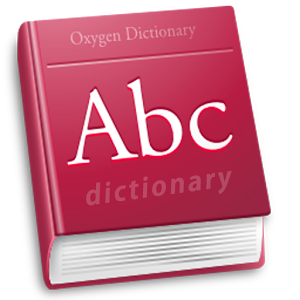
\includegraphics[width=3em]{/home/emarquer/InternshipSynalp2018/report_internship/images/tool_translate_offline_dictionary.png}
}

\begin{tikzpicture}[shorten >=2pt,->,draw=black, node distance=7em]
    \tikzstyle{every pin edge}=[<-,shorten <=2pt]
	\tikzstyle{module}=[minimum size=3em, fill=gray!50!]
	\tikzstyle{char}=[module, circle, fill=green!50!]%, label={below:\usebox\mydictbox}]
	\tikzstyle{text label}=[rectangle, text centered, text width=7em, node distance=5em]
	\tikzstyle{nn}=[rectangle, module, fill=orange!50!]
	\tikzstyle{rnn}=[nn, fill=red!50!]

	\node[char] (char) {\$};
	\node[nn, right of=char] (emb) {Emb.};
	\node[rnn, right of=emb] (rnn) {LSTM};
	\draw[->] (rnn.north) to [out=90,in=90, looseness=2] ($(rnn.west) + (-0.5,0)$) to [out=-90,in=-90, looseness=2] (rnn.south);
	\node[nn, right of=rnn] (lin) {Lin.};
	\node[char, right of=lin] (out) {P(\$$_{+1}$)};
	\draw[->] (char) to (emb);
	\draw[->] (emb) to (rnn);
	\draw[->] (rnn) to (lin);
	\draw[->] (lin) to (out);
	%\node[char] (char) {\$};


    \node[text label, above of=char] (charl) {Caract\`{e}re};
    \node[text label, above of=emb] (embl) {Encodage du caract\`{e}re};
    \node[text label, above of=rnn] (rnnl) {RNN};
    \node[text label, above of=lin] (linl) {Transformation en distribution de probabilit\'{e}};
    \node[text label, above of=out] (outl) {Probabilit\'{e} d'apparition des caract\`{e}res};
\end{tikzpicture}}
	\caption[Architecture du \glsentrytext{model} réimplémenté]{Architecture du \gls{model} réimplémenté. Le modèle prend en entrée des caractères, et produit des probabilités sur quel caractère apparaîtra ensuite.}\label{fig:reimplement}
\end{figure}

Le module d'encodage des caractères, appelé \foreign{embeding layer} en anglais (littéralement \og couche d'inclusion\fg{}), produit une représentation apprise de chaque caractère sous forme de \gls{tensor}. Ce \gls{tensor} est appelé \gls{embedding}. Ce module, entraîné, peut apprendre des propriétés spécifiques à chaque caractère. Par exemple ce module peut apprendre que telle lettre est une consonne et que telle autre est un caractère de ponctuation. \label{def:embeding}

Le \gls{rnn} traite les caractères sous forme de séquence, et peut ainsi apprendre la structure en mots, la syntaxe et d'autres propriétés du langage.

Le module produisant la distribution de probabilité est un module linéaire.
Il transforme les informations produites par le réseau de neurones en probabilité pour chaque caractère d'être le prochain caractère de la séquence. % TODO def module linéaire

Voir les annexes \ref{subsec:testreimp_1}, \ref{subsec:testreimp_2} et \ref{subsec:testreimp_3} pour les rapports sur le \gls{model} ré-implémenté. 

\subsubsection{Conclusion}
Cette étape, outre la préparation du code, à permit la mise en œuvre et une meilleur compréhension des concepts appris durant l’étape précédente. C'est la première pierre de l'édifice qu'est le \gls{gmsnn}. % reprise sur de l'existant, découverte de la lib
\newpage
\subsection{Implémentation du nouveau modèle}
\subsubsection{Travail effectué}
La troisième partie du projet à été la réalisation d'un prototype de l'architecture \gls{gmsnn}, basé sur la ré-implémentation simplifiée du \gls{model} \gls{soa}.

L'architecture du \gls{gmsnn} est identique à celle du \gls{model} ré-implémenté, mis à part le \gls{rnn} qui est remplacé par le \gls{module_gmsnn} (voir \autoref{fig:reimplement_gmsnn}). C'est sur ce nouveau module que le reste du travail au cours du \gls{project_gmsnn} à été effectué.

\begin{figure}[ht]
	\centering
	\scalebox{1}{\usetikzlibrary{calc}

\begin{tikzpicture}[shorten >=2pt,->,draw=black, node distance=7em]
    \tikzstyle{every pin edge}=[<-,shorten <=2pt]
	\tikzstyle{module}=[minimum size=3em, fill=gray!50!]
	\tikzstyle{char}=[module, circle, fill=green!50!]%, label={below:\usebox\mydictbox}]
	\tikzstyle{text label}=[rectangle, text centered, text width=7em, node distance=5em]
	\tikzstyle{nn}=[rectangle, module, fill=orange!50!]
	\tikzstyle{rnn}=[nn, fill=red!50!]

	\node[char] (char) {\$};
	\node[nn, right of=char] (emb) {Emb};
	\node[rnn, right of=emb] (rnn) {GMSNN};
	\draw[->] (rnn.north) to [out=90,in=90, looseness=2] ($(rnn.west) + (-0.5,0)$) to [out=-90,in=-90, looseness=2] (rnn.south);
	\node[nn, right of=rnn] (lin) {Lin};
	\node[char, right of=lin] (out) {P(\$$_{+1}$)};
	\draw[->] (char) to (emb);
	\draw[->] (emb) to (rnn);
	\draw[->] (rnn) to (lin);
	\draw[->] (lin) to (out);
	%\node[char] (char) {\$};


    \node[text label, above of=char] (charl) {Caract\`{e}re};
    \node[text label, above of=emb] (embl) {Encodage du caract\`{e}re};
    \node[text label, above of=rnn] (rnnl) {RNN};
    \node[text label, above of=lin] (linl) {Transformation en distribution de probabilit\'{e}};
    \node[text label, above of=out] (outl) {Probabilit\'{e} d'apparition des caract\`{e}res};
\end{tikzpicture}}
	\caption[Architecture du \glsentrytext{model} réimplémenté]{Architecture du \gls{model} réimplémenté. Le modèle prend en entrée des caractères, et produit des probabilités sur quel caractère apparaîtra ensuite.}\label{fig:reimplement_gmsnn}
\end{figure}

Ce prototype est une implémentation naïve de l'architecture, permettant de mettre en place les mécanismes de base du modèle.

Durant cette étape, nous avons mis en place l'architecture multi-échelle avec deux mécanisme fondamentaux: la transmission de l'information d'une échelle à l'autre, et l'agrégation de l'information de toutes les échelles.

Chaque couche de l'architecture (chaque \og échelle\fg{}) est un \gls{lstm}. \label{def:lstm_2}

\subsubsection{Transmission d'information}
La transmission d'information se fait d'une couche à la couche supérieure.
Cette transmission se fait périodiquement, en fonction d'un nombre appelé fréquence de transmission.

Par exemple, pour fréquence de transmission de $3$~: 
\begin{itemize}
	\item toutes les $3$ entrées de la couche $n-1$, la couche $n$ reçoit de l'information de la couche $n-1$~;
	\item toutes les $3$ entrées de la couche $n$ (soit toutes les $3^2$ entrées de la couche $n-1$), la couche $n+1$ reçoit de l'information de la couche $n$.
\end{itemize}

\vspace{1em}
Dans un premier temps, il à fallu choisir quelle information transmettre d'une échelle à l'échelle supérieure. En effet, les \glspl{rnn} produisent à la fois une sortie, et un \gls{hidden state}. L'utilisation de l'\gls{embedding} à été écarté initialement, car elle n'est pas en accord avec l'architecture proposée.

Le choix s'est porté sur l'\gls{hidden state}, qui contient les informations abstraite de la séquence de caractères, contrairement à la sortie qui contient les informations sur le caractère suivant uniquement.

%TODO passer + sur transmission


Ensuite, il à fallu déterminer comment regrouper les informations avant de les transmettre au module produisant la distribution de probabilité.

%\begin{figure}[h]
%	\begin{subfigure}{0.45\textwidth}
%		\centering
%%		\scalebox{1}{\usetikzlibrary{calc}

\begin{tikzpicture}[shorten >=2pt,->,draw=black!50, node distance=7em]
    \tikzstyle{every pin edge}=[<-,shorten <=2pt]
	\tikzstyle{module}=[minimum size=3em, fill=gray!50!]
	\tikzstyle{char}=[module, circle, fill=green!50!]
	\tikzstyle{text label}=[rectangle, text centered, text width=7.5em, node distance=7em]
	\tikzstyle{nn}=[rectangle, module, fill=orange!50!]
	\tikzstyle{rnn}=[nn, fill=red!50!]

	\node[rnn, pin={[pin edge={<-}, pin distance=3em]south:Entr\'{e}e}] (rnn1) {RNN};
	\node[rnn, above of=rnn1] (rnn2) {RNN};
	\node[rnn, above of=rnn2, pin={[pin edge={->,dashed}, pin distance=3em]north:}] (rnn3) {RNN};

	\foreach \n in {1,...,3}
		\draw[->] (rnn\n.east) to [out=0,in=0, looseness=2] ($(rnn\n.south) + (0,-.5)$) to [out=180,in=180, looseness=2] (rnn\n.west);

	\path[->,dashed] (rnn1)  edge coordinate (@aux) (rnn2);
	\path [late options={name=@aux, pin={[pin edge={-}, text width=10.5em, pin distance=5em]0:Transmission toutes les $n$ entr\'{e}es de l'\'{e}chelle 1}}];
	\path[->,dashed] (rnn2)  edge coordinate (@aux) (rnn3);
	\path [late options={name=@aux, pin={[pin edge={-}, text width=10.5em, pin distance=5em]0:Transmission toutes les $n$ entr\'{e}es de l'\'{e}chelle 2}}];

	\foreach \n in {1,...,3}
	    \node[text label, left of=rnn\n] (rnn\n l) {\'{E}chelle \n};
	\node[right of=rnn3, node distance=10.7em, text width=11em, yshift=3em] (rnn l) {$n$ est la fr\'{e}quence de transmission};
\end{tikzpicture}}
%		\caption{Architecture en blocs simples}
%	\end{subfigure}
%	\begin{subfigure}{0.45\textwidth}
%		\centering
%%		\scalebox{1}{\input{plots/base_gmsnn_unfolded}}
%		\caption{Architecture en blocs dépliés}
%	\end{subfigure} 
%	\caption[Architecture fondamentale du \glsentrytext{gmsnn}]{Architecture fondamentale de \gls{module_gmsnn}}\label{fig:module_gmsnn_base}
%\end{figure}

Voir l'annexe \ref{subsec:testms} pour le rapport sur le prototype. 

\subsubsection{Conclusion}
Cette partie du projet à permit la mise en œuvre de l'architecture proposée. La dernière étape est d'améliorer les performances du modèle, et de l'optimiser. % reprise sur de l'existant
\subsection{Optimisation et amélioration du nouveau modèle}
%TODO passer add to cat dans cette partie ?

%opti 1
	%addcat
	%reprise train
	%batch
%pb mémoire (beaucoup d'opti perf nécessite d'augmenter la taille des params/modules/tenseurs...) & tps (la plupart des otpis perfs augmentent le tps de calcul nécessaire, et de base le modele naif est trop lent)
%pb memoire réglé, tentative infructueuse d'améliorer les perfs avec améliorations préparées en parallèle
	%+ params
	%lbl
% ccl plus pb mémoire & tps, opti z'oignons (XD) même, 5 min c'est balèze

Une fois le prototype fonctionnel, il à fallu améliorer les performances.
Par performances, nous entendons principalement le temps nécessaire pour que la qualité prédictive du modèle dépasse un certain seuil.

Pour améliorer ce temps de calcul, il est possible de travailler sur deux dimensions~:
\begin{itemize}
	\item la \textbf{quantité de données} traitées en un laps de temps~; c'est une \textbf{stratégie quantitative}~;
	\item la \textbf{qualité} de l'apprentissage pour une quantité fixée de données~; c'est une \textbf{stratégie qualitative}.
\end{itemize}

Ainsi, plusieurs options sont possible~:
\begin{itemize}
	\item optimiser les algorithmes et le modèle pour réduire le temps nécessaire pour traiter les données~;
	\item améliorer le modèle en réglant les paramètres (comme la fréquence de transmission) ou en implémentant de nouvelles mécaniques~;
\end{itemize}
\hspace{1em}

Les deux stratégies ont été utilisées. Il faut noter que certaines améliorations qualitatives ont un impact quantitatif négatif.

Principalement, le travail effectué pendant cette partie du projet est un travail de débogage et d'analyse et d'optimisation, avec peu d'implémentation de nouvelles mécaniques dans le \gls{model}.

\subsubsection[Agrégation des sorties des couches]{Agrégation des sorties des couches~: d'une stratégie additive à une concaténation}
La première optimisation à été de changer la façon de regrouper les informations de toues les \og échelles\fg{} avant de les transmettre au module produisant la distribution de probabilité.

Initialement, les sorties de toues les \og échelles\fg{} étaient sommées. Cela permettait de maintenir des \glspl{tensor} de dimensions uniformes quel que soit le nombre d'\og échelle\fg{} (\autoref{fig:add}).

Après discussion avec notre maître de stage, la stratégie d'agrégation à été changé en une concaténation des sorties (\autoref{fig:cat}).

\begin{figure}[ht]
	\begin{subfigure}{0.45\textwidth}
		\centering
		\scalebox{1}{\input{plots/add}}
		\caption[Stratégie d'agrégation additive]{Stratégie d'agrégation additive.\vspace{2em}}\label{fig:add}
	\end{subfigure}
	\begin{subfigure}{0.45\textwidth}
		\centering
		\scalebox{1}{\input{plots/cat}}
		\caption[Stratégie d'agrégation par concaténation]{Stratégie d'agrégation par concaténation. Les sorties sont mises côte-à-côte affin de former un nouveau \gls{tensor}.}\label{fig:cat}
	\end{subfigure} 
	\caption{Stratégies d'agrégation}
\end{figure}

La stratégie par concaténation est plus lente en terme de temps de calcul que la stratégie additive, cependant pour le même temps de calcul elle permet d'obtenir de meilleurs résultats (\autoref{fig:addcat}).

Voir l'annexe \ref{subsec:addcat} pour plus de détail sur le choix de la stratégie d'agrégation. 

\begin{figure}[H]
	\centering
	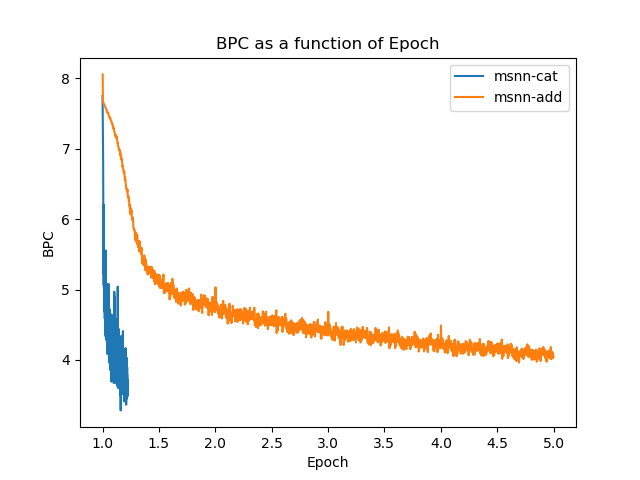
\includegraphics[width=\textwidth]{parts/appendix/reports-gmsnn/docs_esteban-latex/test_reports/comparative-bpc-msnn-det-msnn-cat.png}
	\caption[Performances comparées des stratégies additive et par concaténation]{Performances comparées des stratégies par concaténation (msnn-cat) et additive (msnn-add). Le temps de calcul alloué est identique. Avec la concaténation on entraîne le modèle sur 1/4 des données, avec l'addition on l'entraîne 5 fois sur l'ensemble des données. Avec la concaténation, on obtient une BPC de 3.5, alors qu'on obtient une BPC de 4 avec l'addition.}\label{fig:addcat}
\end{figure} % new

\subsubsection{Sauvegarde, interruption et reprise de l'entraînement}
Une fonctionnalité s'est très vite détachée comme essentielle~: la sauvegarde du \gls{model} et la reprise de l'entraînement.

En effet, avec des entraînements très lents et donc longs, il était nécessaire de pouvoir suspendre l'entraînement affin de répartir le temps de calcul sur plusieurs session de plusieurs heures. De plus, les sauvegardes permettent de conserver le modèle une fois entraîné.

Le système implémenté permet d'effectuer cycliquement des sauvegarde du modèle ainsi que de l'état de l'entraînement, permettant ainsi une reprise en l'état de l'entraînement.

Pour la réalisation du système, le principal obstacle à été le malfonctionnement initial des outils fournis par \gls{pytorch}.
Cela à poussé à la conception d'un système de sauvegarde personnalisé mais malheureusement assez complexe.
Cependant, la mise-à-jour majeure de la librairie qui c'est déroulé à point nommé à résolu le problème, et c'est avec les outils de \gls{pytorch} que le système de sauvegarde à été implémenté.

Voir l'annexe \ref{subsec:save} pour un rapport contenant plus de détail sur le système de sauvegarde. % new
\subsubsection{Tentatives d'optimisations, fuites mémoires et lenteur de l'entraînement}\label{subsec:optimem}

Les optimisations tentées par la suite ont révélé des fuites mémoires et mis en avant une lenteur excessive de l'apprentissage.

Les optimisations en questions ont été mises en suspens le temps de la résolution de ces deux problèmes.
Ces optimisations sont:
\begin{itemize}
	\item l'utilisation de \glspl{batch} simultanés (voir \autoref{subsec:optibatch})~; 
	\item l'augmentation du nombre de \glspl{parameter} du \gls{model} (voir \autoref{subsec:optiparam})~;
\end{itemize}

%\hspace{1em}
\paragraph{Consommation de mémoire et de temps de calcul accrue}
Un effet direct de ces optimisations est l'augmentation de la consommation mémoire.

Cette consommation accrue à causé le plantage de plusieurs tests, révélant la présence de fuites mémoires critiques.
Un ralentissement progressif de l'entraînement à aussi été découvert pendant l'analyse des plantages. % TODO reformuler
Le plus surprenant a été la corrélation forte découverte entre le temps de calcul et la consommation de mémoire.

Un premier correctif à fourni une amélioration notable mais insuffisante.
Il remplaçait le \gls{lstm} de chaque couche (voir \autoref{def:lstm_2}) par un \gls{rnn} basique, moins gourmand. %TODO parler de la redondance 

\paragraph{Estimation de la consommation normale du modèle}
La première étape, qui est détaillée dans l'annexe \ref{subsec:memuse}, à été d'estimer l'usage normal de la mémoire sans fuite, et d'isoler les \glspl{parameter} qui ont le plus d'impact sur la consommation mémoire.
Cela à confirmé que l'explosion de la consommation n'était pas du à l'architecture en elle même, et qu'il s'agissait bien d'une anomalie.

\paragraph{Résolution des fuites}
L'analyse et la résolution des fuites mémoires s'est révélée ardue. Si quelques fuites mineures ont été simple à détecter et réparer, la principale fuite était due à une spécificité non documenté de \gls{pytorch}.

En effet, \gls{pytorch} utilise la \gls{automatic differentiation} pour mettre à jour les \gls{weight} du \gls{nn}.
Pour cela, \gls{pytorch} à besoin de connaître la suite d'opérations et l'implication des différents \glspl{parameter} du \gls{model} et se base sur un \og graphe de computation\fg{}.
C'est la façon dont est gérée ce graphe, couplée aux spécificités de l'architecture \gls{gmsnn} qui est la cause de la principale fuite mémoire.

L'annexe \ref{subsec:memleak} contient une des tentatives de résolution du problème.

% TODO parler de la perf bonasse

\paragraph{Conclusion}
Le problème de la fuite mémoire à été résolu, et avec lui celui de la lenteur de l'entraînement.
On peut déplorer de ne pas avoir analysé plus avant cet étrange lien entre la mémoire et le temps d'entraînement.
Cependant, la résolution des fuites mémoires et de la lenteur de l'entraînement était l'objectif principal de cette étape, et l'optimisation du \gls{module_gmsnn} à pu reprendre. % opti
\subsubsection{Entraînement par exemples simultanés ; \Glsentrytext{batch}} \label{subsec:optibatch}
Une fois le problème des fuites mémoires résolu, la première optimisation mise en place est l'utilisation de \glspl{batch} parallèles.

\paragraph{\gls{batch}}
Un \gls{batch} (anglais pour lot), est un groupe d'exemples successifs.

Le découpage des données en \glspl{batch} permet de répartir l'apprentissage tout au long de l'étude des données.
Cela permet d'atteindre de meilleurs performances.

Il s'agit d'une optimisation rependue pour l'entraînement de \glspl{nn}. % TODO ajouter sources
Elle est souvent couplée à un entraînement simultané sur plusieurs \glspl{batch}.

\paragraph{\Glspl{batch} parallèles}
Un entraînement par \glspl{batch} parallèles permet de calculer le résultat de plusieurs exemples simultanément.
On calcule ensuite la différence de chaque résultat avec le résultat attendu correspondant.
Enfin, on met à jours le \gls{model} en fonction de l'ensemble des exemples.
Au final, les calculs des résultat sont parallélisé, et le coût de la mise à jour est mis en commun entre plusieurs exemples.

Cela permet de réduire drastiquement le temps de calcul et d'améliorer la qualité de l'entraînement, au prix d'une plus grande utilisation de la mémoire.

\paragraph{Conflit entre les \glspl{batch} parallèles et l'architecture \gls{gmsnn}}
Cependant, le découpage en \glspl{batch} pose un problème majeur avec l'architecture \gls{gmsnn}~: elle est basée sur la continuité des exemples fournis, et l'utilisation de \glspl{batch} brise la continuité en introduisant un parallélisme.

Une analyse approfondie à permit d'établir une méthode pour contourner et compenser la majorités des aspect du problème.

Voir le rapport de l'annexe \ref{subsec:batch} pour les détails de l'analyse des problèmes théoriques de l'utilisation de \glspl{batch} avec l'architecture \gls{gmsnn}.

Voir l'annexe \ref{subsec:memuse} pour les détails sur l'impact de la taille des \glspl{batch} et du nombre de \glspl{batch} sur la consommation mémoire.

Voir les annexes\ref{subsec:batch_1}, \ref{subsec:batch_2}, \ref{subsec:batch_3} et \ref{subsec:batch_4} pour les rapports des tests sur la rotation des \glspl{batch}.

\paragraph{Conclusion}
Les problèmes liés à l'utilisation de \glspl{batch} ont été en majorité résolus ou écartés. Après consultation avec notre maître de stage, nous avons décidé d'utiliser l'entraînement par \glspl{batch} malgré les problèmes restants. % new
%nouvelle tentative augmenter params
%aucun impact probant malgré tentative variées
\subsubsection{Augmentation du nombre de paramètres}\label{subsec:optiparam}
Les \glspl{parameter}, ou \glspl{weight}, du modèle sont des valeurs qui varient au long de l'entraînement du \gls{model}. On peut dire que ce sont ces valeurs qui \og apprennent\fg{}.

Le fait d'augmenter ces \glspl{parameter} augmente la qualité de l'apprentissage, et la précision du modèle appris. Mais cela se fait au coût d'un volume plus important du \gls{model}, et d'une augmentation des calculs nécessaires pour utiliser et entraîner le \gls{model}. Cela se manifeste par un entraînement plus lent et une consommation mémoire plus élevée.

Cependant, grâce aux optimisations mises en place durant la résolution des fuites mémoires (voir \autoref{subsec:optimem}), ces coûts ne sont plus dramatiques.

Il existe plusieurs façon de mettre en place cette optimisation~:
\begin{itemize}
	\item augmenter le nombre de neurones par couches~;
	\item augmenter le nombre de couches dans le \glspl{rnn} qui compose chaque \og échelle\fg{}.
\end{itemize}

\paragraph{Conclusion}
Ces deux pratiques ont été testées, et aucune n'apporte d'amélioration de qualité de l'apprentissage, tout en multipliant le temps d'entraînement.
En résumé, ces améliorations apportent des coûts supplémentaires sans aucun bénéfices. % opti
% dernière opti
% algo type EM
% légère amélioration tps de calcul -> graphe
% pas d'améliorattion de perf ->
% révèle pb majeur: seule la première couche semble apprendre -> à priori 90% de l'info est niveau morphologique et syntaxique
\subsubsection{Augmentation du nombre de paramètres}\label{subsec:optilbl}
La dernière optimisation mise en place est un nouvel algorithme d'entraînement.

Cet algorithme est une implémentation naïve d'un entraînement couche par couche appliqué à l'architecture \gls{gmsnn}. Cette algorithme s'apparente aux algorithmes HM \autocite{hm}.

L'intuition à l'origine de l'algorithme est~:
il semble que pour apprendre des représentations de haut niveau, le modèle doit en premier lieu apprendre les représentations de bas niveau~;
en effet, sans mots, il est difficile de faire des phrases cohérentes.

Cela sous-entend que les échelles les plus proches des données doivent apprendre avant que les échelles supérieures puisse apprendre.
Aussi, il semble inutile d'augmenter la charge de l'algorithme d'entraînement en entraînant des couches qui n'apprennent pas.

Le fonctionnent général de cette algorithme est d'entraîner successivement, une à une, les échelles du \gls{model} en commençant par celle la plus proche des données.

Le fonctionnement détaillé de l'algorithme est disponible dans l'annexe \ref{subsec:lbl}.

\paragraph{Performances}
Les performances de l'algorithme sont disponible dans le rapport dans l'annexe \ref{subsec:test_perf}.

L'algorithme remplis sa fonction d'alléger la charge calculatoire. En effet, on à une réduction notable du temps nécessaire pour l'entraînement. % TODO parler de temps constant

De plus, il n'y à aucune variation notable de la qualité de l'entraînement.

%\paragraph{Seule la première couche du modèle semble apprendre}
Justement, comme seule une échelle apprend, on pourrait s'attendre à une baisse des performances.% TODO dire pourquoi.

Comme le \gls{model} muni d'une seule échelle apprend aussi bien que le \gls{model} multi-échelles, cela remet en question l'utilité de l'architecture \gls{gmsnn} et de ses échelles multiples.

\paragraph{Conclusion}
 % new/opti

\subsubsection{Conclusion}
Cette partie du \gls{project_gmsnn} à permit d'améliorer notablement les performances du \gls{model}, tout en réduisant drastiquement le coût d'entraînement.% ccl plus pb mémoire & tps, opti z'oignons (XD) même, 5 min c'est balèze

De plus, l'algorithme présenté \autoref{subsec:optilbl} à démontré une faiblesse majeure de l'architecture \gls{gmsnn}.

On peut aussi noter la mise-à-jour majeure de \gls{pytorch}, qui en plus de résoudre certains dysfonctionnements à nécessité le remaniement d'une partie de la base de code.
 % Optimisation et amélioration du nouveau modèle
\subsection{Production des exemples et découverte du problème d'encodage}
Une fois le modèle fonctionnel, une partie importante de la compréhension et de l'évaluation du modèle est la production d'exemple.

Nous avons retardé cette étape principalement à cause des problèmes de mémoire.

Le principe de cette étape est d'utiliser notre \gls{lm} pour produire du langage, afin d'avoir une idée plus concrète qu'un score de la performance du modèle.

\subsubsection{Exemples}
Voici quelques exemples produits par le modèle. 
La version du modèle choisie est celle avec le meilleur score, parmi celle enregistrées.

Age du modèle~: 465 époques.

Score BPC du modèle~: 1.839.

Pour comparaison, le modèle \gls{soa} avait un score BPC de 1.255 en 50 époques.

Pour rappel, les données sont issues d'une version filtrée de Wikipédia en anglais.

%longstring
\begin{lstlisting}[caption={Exemple 1~: une suite de caractères à priori incompréhensibles.},label=gmsnn_ex1]
YeoMMDF|Ph#elementat[[Damous]]thatureoftenusevoirbeexpounderstatesandanumberofhisworkformembersothan novelwasmethecebylementorfromthelastPreenancenoldWarInstartedbythe Philosophy''theTayita(amsmethouspeopleamingshelebelobesinthesatietheuniversalistscientis educationof[[Lakingforts]].
\end{lstlisting}

%good
\begin{lstlisting}[caption={Exemple 2~: des termes balisé comme dans le corpus d'origine, les crochets ouverts sont refermés.},label=gmsnn_ex2]
+EDrFuergCases,areinlesssuchasthesthealterplains.
*In[[Stefapes]]
*[[AcademyAwards===

ANASA)asLASCIIRunder,andas.MatthebusipenclearsandpresidenthaveaquelfuelsifthesearchfromAwarerLievol ofany30020.

It''[[Anim]]
*[[UnitedStates|raphicsiteDirection]]

Theplant-gainheditsreturnedtoaseethewarinsteast&quot;Oneofthe[ectlywouldnotbytheIntegrationscapianland](ora''[[schology]]
|published:
\end{lstlisting}

%longstring + tags
\begin{lstlisting}[caption={Exemple 3~: des termes balisé comme dans l'exemple 2, et une autre suite de carractères.},label=gmsnn_ex3]
60447-toNewHarry}}
Thenmainst.Rand'sintereststhe&quot;toinpassingtheEarth''s(''[[par]].

:'''maimals,anackreloquedoutwidthofgrawwithluteframedapproyingtoundernverby[[hebesination]]of&lt;/smalkan,instablishedacondorttodevelopedframesbeforestatedwinkingaroundinrational hicarefartoredonaftercanbeagainsthatgroupswouldnear,notwhatwasthatisstillastructionCenter,toDagnythat

On[[teleofAirëejã]]
[[cy:Alaska]]
[[no:Arni-Anchorages]]
\end{lstlisting}

\subsubsection{Manque d'espaces}
Parmi ces exemples, on remarque immédiatement le manque d'espace.

La source de ce phénomène n'est autre qu'un problème dans le corpus source.
La version pré-traitée de ce corpus ne contenait aucun espace, donc le \gls{model} à appris une langue dans laquelle l'espace n'existe pas.

C'est un problème majeur, qui à probablement eu un impact élevé sur les performances du modèle. En effet, en anglais comme dans beaucoup de langues occidentales, l'espace est un élément fondamental dans la structuration du langage écrit. Le \gls{model} à ainsi apprit une langue moins structurée, donc plus difficile à apprendre, que l'anglais.

\subsubsection{Quelque éléments qui ressortent}
Cependant, si on regarde plus en détail les exemples produits, des structures apparaissent. 

Si on prend \lstinline!*[[UnitedStates|raphicsiteDirection]]! de l'exemple 2 (\autoref{gmsnn_ex2}, ligne 8) ou 
\lstinline![[cy:Alaska]]! et \lstinline![[no:Arni-Anchorages]]! de l'exemple 2 (\autoref{gmsnn_ex2}, lignes 7 et 8), on a des doubles crochets, qui sont correctement ouverts puis fermés. On remarque aussi la présence de séparateurs (\lstinline!:! et \lstinline!|!).

Ces structure sont similaire aux annotations présentes dans le code Wikipédia.

Enfin, malgré l'absence d'espaces, on discerne de nombreux mots~:
\begin{itemize}
\item la suite de mots \lstinline!statesandanumberofhisworkformembersothannovelwasmethe! qui ne contient en fait que des mots bien formés en anglais~: \lstinline!states and a number of his work for member so than novel was me the! (\autoref{gmsnn_ex1}, ligne 1);
\item de même pour la suite de mots \lstinline!oldWarInstartedbythePhilosophy!~: \lstinline!old War In started by the Philosophy! (\autoref{gmsnn_ex1}, ligne 1);
\item on trouve aussi des noms propres comme le nom de pays~: \lstinline!UnitedStates! (\autoref{gmsnn_ex2}, ligne 8) et \lstinline!Alaska! (\autoref{gmsnn_ex3}, ligne 7).
\end{itemize}
\section{Analyse des résultats et arrêt du projet}\label{white_flag}
% Durant la periode d'optimisations, j'avais préparé plein de trucs
% Je les ai tous testés: aucun changement de perf, légère opti tps

% Ca + tout "corrompu" par dataset foiré

% + Retour de réunion sur papud
% => arret du projet et passage sur papud
% gmsnn opti, mais pas assez performant

\subsection{Analyse des résultats}
Avec notre maître de stage, nous avons étudié attentivement les résultats des dernières optimisations sur les performances du \gls{model} (voir annexe \ref{subsec:test_perf}). 
Le résultat le plus dérangeant était l'absence d'apprentissage des couche supérieures.

À partir des connaissances de la littérature possédées par notre maître de stage et de ce résultat, nous avons conclu que 90\% de l'information nécessaire est apprise par la première échelle du modèle. Les autres échelles ne font qu'améliorer ce résultat, et sont peu utiles tant que la première échelle n'est pas complètement entraînée.

À cela s'ajoute la disparition des espaces du corpus, qui nécessiterait non seulement de remanier une partie du code tenue pour acquise, mais aussi de refaire la plupart des tests effectués.

\subsection{Conclusions de l'analyse}
La conclusion à laquelle nous sommes arrivés est qu'il aurait fallu recommencer le développement avec un système de gestion des données maîtrisé et changer le processus de développement du modèle.

La première étape aurait été de développer un modèle simple, avec une seule échelle, et de le pousser au maximum de ses capacités. Seulement à ce moment là nous aurions pu l'augmenter d'autres échelles.

Il aurait aussi été intéressant de revoir l'architecture pour utiliser un modèle sans récurrences.

Cette conclusion impliquait de recommencer le projet, ou à défaut de le remanier en grande partie.

\subsection{Arrêt du projet et début du projet suivant}
Au moment de cette analyse, notre maître de stage revenait d'une réunion décisive sur le \gls{project_papud}.

Celle-ci avait permis de définir les objectifs du \glsfirst{project_papud} (voir \autoref{ch:project_papud}), qui ont été influencés par nos conclusions.

La nécessité de recommencer le \gls{project_gmsnn}, couplée à l'opportunité de mettre les conclusions et les compétences acquises en pratique dans un projet à grande échelle, nous ont mené à interrompre \gls{project_gmsnn} pour consacrer la fin du stage au \gls{project_papud}.

C'est d'un commun accord avec notre maître de stage que nous avons décidé de basculer sur le \gls{project_papud}.
\subsection{Conclusions}
% TODO production des résultats -> nospace
Ce projet nous à permit d'implémenter une architecture innovante de \gls{nn}, à partir d'un modèle état de l'art.

% ccl plus pb mémoire & tps, opti z'oignons (XD) même, 5 min c'est balèze
C'est la première pierre de l'édifice qu'est le \gls{gmsnn}.
mise en œuvre de l'architecture proposée. La dernière étape est d'améliorer les performances du modèle, et de l'optimiser.
Cette partie du \gls{project_gmsnn} à permit d'améliorer notablement les performances du \gls{model}, tout en réduisant drastiquement le coût d'entraînement.

De plus, l'algorithme présenté \autoref{subsec:optilbl} à démontré une faiblesse majeure de l'architecture \gls{gmsnn}.
La réalisation de ce projet nous à permit d'approfondir largement nos connaissances en \gls{dl}. 


\section{\Glsentrytext{project_papud}}
\subsection{Recherche documentaire} % lib, tutos, concepts
\subsection{Ré-implémentation simplifiée du modèle \glsentrytext{soa}} % reprise sur de l'existant, découverte de la lib
\subsection{Implémentation du nouveau modèle basique} % reprise sur de l'existant
\subsection{Optimisation et amélioration du nouveau modèle}
\subsection{Conclusions}


\section{Documentation}


%Il est aisé d'insérer du code dans un rapport. Il suffit de définir le langage, la légende à afficher et enfin un Label pour pouvoir y faire référence. Le résultat est donnée dans le listing \ref{lst:premierExemple}. Il est également possible de changer les couleurs, pour cela il faut éditer le lstset dans la classe tnreport.cls.

%\begin{lstlisting}[language=c++, caption={Premier Exemple}, label={lst:premierExemple}]
%void CEquation::IniParser()
%{
%if (!pP){ //if not already initialized...
%pP = new mu::Parser;
%
%pP->DefineOprt("%", CEquation::Mod, 6); //deprecated
%pP->DefineFun("mod", &CEquation::Mod, false);
%pP->DefineOprt("&", AND, 1); //DEPRECATED
%pP->DefineOprt("and", AND, 1);
%pP->DefineOprt("|", OR, 1); //DEPRECATED
%pP->DefineOprt("or", OR, 1);
%pP->DefineOprt("xor", XOR, 1);
%pP->DefineInfixOprt("!", NOT);
%pP->DefineFun("floor", &CEquation::Floor, false);
%pP->DefineFun("ceil", &CEquation::Ceil, false);
%pP->DefineFun("abs", &CEquation::Abs, false);
%pP->DefineFun("rand", &CEquation::Rand, false);
%pP->DefineFun("tex", &CEquation::Tex, false);
%
%pP->DefineVar("x", &XVar);
%pP->DefineVar("y", &YVar);
%pP->DefineVar("z", &ZVar);
%}
%}
%\end{lstlisting}
%\clearpage
%Il est également possible d'afficher du code directement depuis un fichier source, le résultat de cette opération est visible dans le listing \ref{lst:fromSrc}
%\lstinputlisting[language=c++,caption={Affichage depuis le fichier source},label={lst:fromSrc}]{figures/sourceCode.cpp}\cleardoublepage
	\chapter{Conclusion}


\cleardoublepage
}

{%----- Appendix -----
	
\appendix
%\pagenumbering{Alph}
%\setcounter{page}{1}
%\renewcommand{\thesubsection}{\Roman{subsection}}
%\renewcommand{\thesection}{\Roman{section}}
%\addtocontents{toc}{\protect\pagebreak}

%\addtocontents{toc}{\protect\setcounter{tocdepth}{-1}}
\part*{Annexes\addcontentsline{toc}{chapter}{Annexes}}

\cleardoublepage

\etocdepthtag.toc{mtappendix}
\etocsettagdepth{mtchapter}{none}
\etocsettagdepth{mtappendix}{subsection}
\etoctocstyle{1}{Table des annexes}

\tableofcontents
\cleardoublepage


% Bibliographie
%\renewcommand{\tocbibname}{Bibliographie / Webographie}
%\nocite{*}
%\bibliography{} % See example.bib 
%\bibliographystyle{plain}
\printbibliography[heading=bibintoc]\cleardoublepage
% Liste des figure
%\listoffigures%\cleardoublepage
% Liste des tables
%\listoftables%\cleardoublepage
% Liste des figure
%\lstlistoflistings
\lists
\cleardoublepage
\terms
\cleardoublepage
\captionsetup[figure]{list=no}
\captionsetup[table]{list=no}
\renewcommand\arraystretch{1.5}
\chapter{Rapports d'avancement du \glsentrytext{project_gmsnn}}
%Les rapports ici présenté ont été écrit en langage \gls{md}, plus spécifiquement dans le dialecte nommé \foreign{Gitlab-flavored Markdown}.
%Ce dialecte supporte des éléments comme l'intégration d'images, de formules, de fragments de codes entre autres fonctionnalités.
%Ces spécificités en font un langage idéal pour écrire des rapports exploitants ces fonctionnalités et destinés à être lus au format informatique.
%De plus

\section{Informations sur les rapports contenus dans la présente annexe} \label{report_infos}
Les sections suivantes contiennent les rapports intermédiaires fournis à notre maître de stage au cours du \gls{project_gmsnn}.

\subsection{Format d'origine des rapports}
Le langage \gls{md}, plus spécifiquement dans le dialecte nommé \gls{git_md}, fournit une syntaxe facile à lire et à écrire.%\foreign{Gitlab-flavored Markdown}.
Il permet la rédaction de documents agrémentés entre autres d'images, de formules, de tableaux et de fragments de codes.
Enfin, l'affichage du \gls{git_md} est supporté par \gls{gitlab}. % TODO améliorer phrase

Ces particularités en font un langage de premier choix pour l'écriture de rapports destinés à être lus au format informatique directement sur \gls{gitlab}.

\subsection{Transcription des rapports}
L'intégration des rapports intermédiaires dans ce rapport à nécessité l'adaptation du contenu en \gls{git_md} au format papier.

Certains éléments n'ont pas pu être transcrit tels-quels, en particulier les liens, et les tableaux et images de grand taille.

\subsection{Contenu et langue des rapports}
Le contenu des rapports n'a été ni modifié ni corrigé, et est livré en anglais tel qu'écrit à l'origine.

L'anglais à été choisi comme langue de rédaction des rapports pour maintenir la cohérence avec le code, écrit et documenté en anglais lui aussi, et avec la littérature, principalement rédigée en anglais.
Ce choix évite aussi d'alourdir le contenu déjà complexe des documents avec des traductions maladroites de termes techniques. %TODO Je met fraiment ca ?

\newpage
\begin{report}{Étude des problèmes de mémoire}\label{subsec:memuse}
	% !TeX spellcheck = en_US
\section*{Analysis of memory usage}

Analysis report

by E. Marquer, 2018/05/23, Synalp and Université de Lorraine

\subsection{Abstract}

Experimental results shows (using \lstinline!nvidia-smi!) an increasing
memory usage for 4 layers, from an already enormous 3GB to more than
6GB, causing an out-of-memory error.

The objective of the following computations is to estimate the memory
consumption of the model, to confirm the hypothesis of a memory leak,
and verify that the model should not overflow memory.

\subsection{Formulas}

\subsubsection{Tensor and Variable size
estimation}

Byte size of a tensor is close to 6 times the products of all of its
dimensions. Byte size of a variable is similar to that of the
corresponding tensor.

\begin{lstlisting}[language=Python]
import torch, pickle

# Object to mesure
o = torch.autograd.Variable(torch.ones(100, 100, 100))
o = torch.ones(100, 100, 100)

len(pickle.dumps(o, 0)) / (100 * 100 * 100)
#result = 6
\end{lstlisting}

\subsubsection{Computations}
\vspace{-2em}
\begin{equation}
\begin{aligned}
total 
&= hidden\_states + msnn\_weights + emb\_weights + out\_weights \\\\
&= detach\_interval * (growth\_factor + 1) * layers * 6 * (hidden\_size * batch\_size * sequence\_length) \\
& + (((layer - 1) * 8 * hidden\_size * (hidden\_size + 1)) \\
& + 4 * hidden\_size * (hidden\_size + emb\_size + 2)) * 6  \\
& + (nwords * (emb\_size + 1)) * 6 \\
& + (nwords * (layers * hidden\_size)) * 6 \\\\
&= 6 * (detach\_interval * (growth\_factor + 1) * layers * 
(hidden\_size * batch\_size * sequence\_length) \\
& + ((layers - 1) * 8 * hidden\_size * (hidden\_size + 1)) \\
& + 4 * hidden\_size * (hidden\_size + emb\_size + 2)  \\
& + (nwords * (emb\_size + 1)) \\
& + (nwords * (layers * hidden\_size)))
\end{aligned}
\end{equation}

\begin{equation}
\begin{aligned}
hidden\_states &= total\_history * 6 * dim \\
               &= detach\_interval * (growth\_factor + 1) * layers * 6 * dim \\
               &= detach\_interval * (growth\_factor + 1) * layers * 6 * \\
               & (hidden\_size * batch\_size * sequence\_length)
\end{aligned}
\end{equation}

\begin{equation}
\begin{aligned}
msnn\_layer\_weights &= weights\_ih + weights\_hh + bias\_ih + bias\_hh \\
                     &= 4 * hidden\_size * input\_size + 4 * hidden\_size * hidden\_size \\
                     & + 4 * hidden\_size + 4 * hidden\_size \\
                     &= 4 * hidden\_size * (hidden\_size + input\_size + 2) \\
                     &= \begin{cases}
                        8 * hidden\_size * (hidden\_size + 1) &\text{for all layers exept the first one} \\
                        4 * hidden\_size * (hidden\_size + emb\_size + 2)  &\text{for the first layer}
                        \end{cases}
\end{aligned}
\end{equation}

\begin{equation}
\begin{aligned}
msnn\_weights &= msnn\_layer\_weights * layers \\
              &= ((layers - 1) * 8 * hidden\_size * (hidden\_size + 1))\\
              & + 4 * hidden\_size * (hidden\_size + emb\_size + 2)
\end{aligned}
\end{equation}

\begin{equation}
\begin{aligned}
emb\_weights &= (bias + weights) * 6 \\
            &= (nwords * emb\_size + emb\_size))* 6 \\
            &= (nwords * (emb\_size + 1)) * 6
\end{aligned}
\end{equation}

\begin{equation}
out\_weights = (nwords * (layers * hidden\_size)) * 6
\end{equation}

\newpage
\subsubsection{Estimate with basic set of parameters}

\begin{lstlisting}[language=Python]
detach_interval = 50
growth_factor = 5
layers = 7
hidden_size = 1840 / 4
batch_size = 2
sequence_length = 100
emb_size = 400
nwords = 205

total = 6 * (detach_interval * (growth_factor + 1) * layers * hidden_size * batch_size * sequence_length + ((layers - 1) * 8 * hidden_size * (hidden_size + 1)) + 4 * hidden_size * (hidden_size + emb_size + 2) + (nwords * (emb_size + 1)) + (nwords * (layers * hidden_size)))

"{}GB {}MB {}kB {}B".format(int(total%(1024**4) / 1024**3), int(total%(1024**3) / 1024**2), int(total%(1024**2) / 1024), int(total%1024))
# result: '1GB 741MB 614kB 9B'
\end{lstlisting}

\newpage
\rotatebox{90}{
\begin{tabular}{|cccccccc|r|}
\hline
detach\_interval & growth\_factor & layers & hidden\_size & batch\_size & sequence\_length & emb\_size & nwords & total\\
\hline
50 & 5 & 7 & 1840 / 4 & 2 & 200 / batch\_size & 400 & 205 & 1GB 153MB 68kB 6B\\
\textbf{100} & 5 & 7 & 1840 / 4 & 2 & 200 / batch\_size & 400 & 205 & 2GB 234MB 579kB 262B\\
\textbf{200} & 5 & 7 & 1840 / 4 & 2 & 200 / batch\_size & 400 & 205 & 4GB 397MB 577kB 774B\\
50 & \textbf{10} & 7 & 1840 / 4 & 2 & 200 / batch\_size & 400 & 205 & 2GB 50MB 323kB 390B\\
50 & 5 & \textbf{6} & 1840 / 4 & 2 & 200 / batch\_size & 400 & 205 & 1008MB 912kB 414B\\
50 & 5 & \textbf{5} & 1840 / 4 & 2 & 200 / batch\_size & 400 & 205 & 840MB 732kB 822B\\
50 & 5 & \textbf{4} & 1840 / 4 & 2 & 200 / batch\_size & 400 & 205 & 672MB 553kB 206B\\
50 & 5 & \textbf{3} & 1840 / 4 & 2 & 200 / batch\_size & 400 & 205 & 504MB 373kB 614B\\
50 & 5 & \textbf{2} & 1840 / 4 & 2 & 200 / batch\_size & 400 & 205 & 336MB 193kB 1022B\\
50 & 5 & \textbf{1} & 1840 / 4 & 2 & 200 / batch\_size & 400 & 205 & 168MB 14kB 406B\\
50 & 5 & 7 & \textbf{1840 / 2} & 2 & 200 / batch\_size & 400 & 205 & 2GB 431MB 598kB 94B\\
50 & 5 & 7 & \textbf{1840 / 8} & 2 & 200 / batch\_size & 400 & 205 & 573MB 28kB 890B\\
50 & 5 & 7 & 1840 / 4 & \textbf{1} & \textbf{200 / batch\_size} & 400 & 205 & 1GB 153MB 68kB 6B\\
50 & 5 & 7 & 1840 / 4 & 2 & \textbf{200} & 400 & 205 & 2GB 234MB 579kB 262B\\
50 & 5 & 7 & 1840 / 4 & 2 & 200 / batch\_size & \textbf{200} & 205 & 1GB 150MB 743kB 534B\\
50 & 5 & 7 & 1840 / 4 & 2 & 200 / batch\_size & \textbf{800} & 205 & 1GB 157MB 764kB 998B\\
50 & 5 & 7 & 1840 / 4 & 2 & 200 / batch\_size & 400 & \textbf{500} & 1GB 159MB 182kB 984B\\
\hline
\end{tabular}
}

\newpage
\paragraph{Most impactful factors
(memory-wise)}

\begin{itemize}
\item
  \lstinline!detach_interval!: \lstinline!detach_interval * 2! =
  \lstinline!memory * 2!
\item
  \lstinline!growth_factor!: \lstinline!growth_factor * 2! =
  \lstinline!memory * 2!
\item
  \lstinline!hidden_size!: \lstinline!hidden_size * 2! =
  \lstinline!memory * 2!
\item
  \lstinline!batch_size * sequence_length! (number of examples by
  sequence): \lstinline!batch_size*sequence_length * 2! =
  \lstinline!memory * 2!
\item
  \lstinline!layers!: \lstinline!layers * 2! = \lstinline!layers * 2!
\end{itemize}

The others factors considered (emb\_size and nwords) have almost no
impact on memory. It confirms that the most memoryphage element is the
MSNN. Also, to keep a stable memory usage,
\lstinline!batch_size * sequence_length! ratio must be kept constant;
increasing \lstinline!batch_size! while lowering
\lstinline!sequence_length! can increase processing speed whithout
impacting memory usage.

\subparagraph{Impact of layer increase}
\subparagraph*{}\vspace{-2em}{We can notice that the impacts of layers is most noticeable during the
first phases of training, during the creation of the first layer. Later
on, the creation frequency of new layers is small, and the change is
minimal. For example, from 6 to 7 layer, we need \(`12500`\) sequences
to pass, and the increase of memory of about \(`7/6`\); from 7 to 8
layer, we need \(`62500`\) sequences to pass, and the increase of memory
of about \(`8/7`\); from 8 to 9 layer, we need \(`312500`\) sequences to
pass, and the increase of memory of about \(`9/8`\); and so on.}

\subsubsection{Partial derivatives:}

\begin{lstlisting}
d = detach_interval
g = growth_factor
l = layers
h = hidden_size
b = batch_size
s = sequence_length
e = emb_size
n = nwords

complete formula:
6 * (
	d * (g + 1) * l * h * b * s +
	((l - 1) * 8 * h * (h + 1)) +
	4 * h * (h + e + 2) +
	(n * (e + 1)) +
	(n * (l * h))
)

simplified formula:
6*(8*l*h^2 + l*d*g*h*b*s + l*d*h*b*s + 8*l*h + l*n*h + 4*e*h + e*n + n - 4*h^2)

partial derivates on given variable:
d: (6(8*l*h^2 - 4*h^2 + l*d*g*h*b*s + l*d*h*b*s + 8*l*h + 4*e*h + l*n*h + e*n + n))
g: 6*l*d*h*b*s
l: 6*(d*h*b*s*(g+1) + 8*h*(h+1) + nh)
h: 6*(l*d*g*b*s + l*d*b*s + l*n + 16*l*h + 8*l + 4*e - 8*h)
b: 6*l*d*h*s*(g+1)
s: 6*l*d*h*b*(g+1)
e: 0
n: 6*(l*h+e+1)
\end{lstlisting}


\end{report}
\begin{report}{Sauvegarde du modèle}\label{subsec:save}
	\section*{Analysis and implementation of job save and
restart}

Implementation report

by E. Marquer, 2018/05/24\\
Synalp and Université de Lorraine

\subsection{Abstract}

As the jobs are taking longer than an hour per epoch, it has become
necessary to keep an image of the model, the training parameters and the
current state of the model to be able to interrupt training when needed.

Multiple choices are available:
\begin{itemize}
\item an easy but heavy serialisation (pickle) of the whole system;
\item a ``full'' save of the model and parameters, excluding everything that can be recomputed easily;
\item a ``partial'' save of the model, removing a part of the less important
information.
\end{itemize}

\subsection{\texorpdfstring{\textbf{End solution: saving using pytorch
utilities}}{End solution: saving using pytorch utilities}}

The saving solution currently implemented is the
\lstinline!torch.save(trainer, file)! and
\lstinline!trainer = torch.load(file)! and the alternatie version
\lstinline!trainer = torch.load(file, map_location=lambda storage, loc: storage)!
allowing the loading of a CUDA model out of CUDA.

This solution posed a number of problems when it was first tested
(internal non-parameter atributes where not correctly saved and loaded),
that is why it was not considered at first.

But a more recent try resulted in a perfect result, replacing the need
of a custom serialisation system.

\subsection{Full serialisation}

This kind of serialisation is done thanks the \lstinline!pickle!
package, on the whole Trainer object.

\begin{lstlisting}[language=Python]
import pickle

def load(filename: str) -> object:
    with open(filename, 'rb') as f:
        return pickle.load(f)

def save(filename: str, trainer: object) -> None:
    with open(filename, 'wb') as f:
        pickle.dump(trainer, f)
\end{lstlisting}

\subsection{Full save}

\subsubsection{Elements to save}

\begin{itemize}
\item
  Corpus file name
\item
  \lstinline!cuda_on!
\item
  \lstinline!batch_size!
\item
  Trainer

  \begin{itemize}
  \item
    Model (see specific points)
  \item
    \lstinline!self.epoch! current epoch
  \item
    \lstinline!self.batch! and \lstinline!self.i! current position in
    training epoch
  \item
    \lstinline!self.start_time! needs a litle work: storing the elapsed
    time, and when loading, remove elapsed time from load time
  \item
    \lstinline!self.log_interval!
  \item
    \lstinline!self.save_interval!
  \item
    \lstinline!self.bptt!
  \item
    \lstinline!self.nwords!
  \item
    \lstinline!self.repackage_interval!
  \item
    \lstinline!self.repackage_strategy!
  \item
    \lstinline!self.reset_growth!
  \item
    \lstinline!self.reset_hidden!
  \item
    \lstinline!self.epochs!
  \item
    \lstinline!self.save_folder!
  \end{itemize}
\item
  Model (MSNN)

  \begin{itemize}
  \item
    \lstinline!self.training!
  \item
    input layer (embeddings) using \lstinline!torch.save(self.emb, f)!
    and \lstinline!torch.load(f)!
  \item
    MSNN (see specific points)
  \item
    output layer (linear)
  \end{itemize}
\item
  MSNN

  \begin{itemize}
  \item
    Final

    \begin{itemize}
    \item
      \lstinline!self.input_size!
    \item
      \lstinline!self.hidden_size!
    \item
      \lstinline!self.growth_factor!
    \item
      \lstinline!self.batch_size!
    \item
      \lstinline!self.cuda_on!
    \item
      \lstinline!self.layer_id!
    \item
      \lstinline!self.max_detach!
    \item
      \lstinline!self.repackage_strategy!
    \item
      \lstinline!self.max_layers!
    \end{itemize}
  \item
    Next MSNN
  \item
    \lstinline!self.detach_count!
  \item
    \lstinline!self.rnn!
  \item
    \lstinline!self.hidden!
  \item
    \lstinline!self.seq_count!
  \item
    \lstinline!self.detach_count!
  \item
    \lstinline!self.transmitted_output!
  \item
    \lstinline!self.transmitted_hidden!
  \end{itemize}
\end{itemize}

\subsubsection{Elements to forget and
recreate}

\begin{itemize}
\item
  Trainer

  \begin{itemize}
  \item
    Corpus

    \begin{itemize}
    \item
      Corpus file name is needed
    \end{itemize}
  \item
    Optimizer: reasign learning rate, weight\_decay and model's
    parameters (create after model is loaded) using
    \lstinline!torch.optim.SGD(model.parameters(), lr=args.lr, weight_decay=args.weight_decay)!
  \item
    Criterion: \lstinline!criterion = torch.nn.CrossEntropyLoss()!
  \item
    \lstinline!self.layers! using
    \lstinline!self.model.msnn.get_layers()! (create after model is
    loaded)
  \item
    \lstinline!self.train_data! using
    \lstinline!batchify(corpus.train, batch_size, cuda_on)!
  \item
    \lstinline!self.val_data! using
    \lstinline!batchify(corpus.valid, batch_size, cuda_on)!
  \item
    \lstinline!self.plotdata! using
    \lstinline!{"Epoch": None, "Layer": None, "Frac": None}! and
    \lstinline!self.init_plotter()! (perhaps with a new file, otherwise
    in append mode without cleaning the file)
  \item
    \lstinline!self.msnn_backup!, sould be empty if the new backup
    system (using the \lstinline!with! statement) is implemented
  \end{itemize}
\item
  Model

  \begin{itemize}
  \item
    None
  \end{itemize}
\item
  MSNN

  \begin{itemize}
  \item
    \lstinline!self.tensors!
  \end{itemize}
\end{itemize}

\subsection{Partial save}

The elements to keep are the same as with the Full save, except: -
hidden states and transmitted output are to be detached

\subsection{Other things that need to be added to interrupt and resume
job}

\subsubsection{Methods to interrupt and resume epoch loop and training
loop}

\paragraph{Interruption strategy}

Interruption can be done by:
\begin{itemize}
\item saving the state at specific timestep;
\item saving automatically when shutting down.
\end{itemize}

The second option isn't realy realistic, as an interuption wouldn't
allow a big enough margin to save the model. Even thought, it could be
added to allow manual interruption at certain timesteps (smaller than
the ones implemented in the first option).

As the first option is the only viable one, multiple timesteps are
possible, from the shortest to the longest:
\begin{itemize}
\item after each operation (example: after forward pass, and after backward pass, and after optimization \ldots{});
\item after each sequence;
\item after \emph{n} sequences;
\item  after each epoch;
\item  after \emph{n} epochs;
\item  after the whole training.
\end{itemize}

Option {[}1.{]} is not viable, as it would consume a lot of time
relative to each computation for the sole writing process. Option
{[}3.{]}, of which option {[}2.{]} is a specific case, allows both a
fine granulation with only a minimal loss if anything were to occur, and
a reduced burden computation-wise. From option {[}4.{]} onward, the save
time is negligible, and even if the granulation is mediocre, it offers
fine milestones for specific usage (usage of an already trained mode for
example).

Currently, at creation time, with no history, the model save file is
about 770MB.

What will be implemented is thoe third option, saving the model after
\emph{n} sequences.

\paragraph{Resume strategy}\label{resume-strategy}

It will be necessary to adapt the training loodps a little to allow
resuming at any sequence in any epoch.

\subsection{Other methods implemented}\label{other-methods-implemented}

\subsubsection{\texorpdfstring{Method using \texttt{with} keyword for
backup system, during
evaluation}{Method using with keyword for backup system, during evaluation}}\label{method-using-with-keyword-for-backup-system-during-evaluation}

\begin{lstlisting}[language=Python]
class BackupContextManager:
    def __init__(self, model: DetRNN):
        self.model = model
        
    def __enter__(self):
        # Backing up training linked data
        self.msnn_backup = self.model.msnn.backup()

    def __exit__(self, type, value, traceback):
        # Restoring training linked data
        self.model.msnn.restore(self.msnn_backup)


with BackupContextManager(model):
    """Do computations"""
\end{lstlisting}


\end{report}
\begin{report}{Solution tentative pour les fuites mémoires}\label{subsec:memleak}\label{subsec:hist}
	% !TeX spellcheck = en_US
\section*{Analysis of a source of the memory leak problem: the history
management
system}

Analysis report

by E. Marquer, 2018/05/28, Synalp and Université de Lorraine

\subsection{Abstract}

A big memory leak is present in the model. One of the identified cause
is a malfunction in the history management system.

\subsection{Problem}

It seems simply detaching a hidden state is not enough:

With a graph:
\begin{lstlisting}
                        3.1 --------------------------- 3.2 -->
                         |                               |
        2.1 ----------- 2.2 ----------- 2.3 ----------- 2.4 -->
         |               |               |               |
1.1 --- 1.2 --- 1.3 --- 1.4 --- 1.5 --- 1.6 --- 1.7 --- 1.8 -->
\end{lstlisting}
where all nodes are hidden states, and each layer is a line, with a
transmission rate of 1 transmission every 2 hidden state.

When detaching every 2 hidden, with \lstinline![i.j]! a detached node,
the graph becomes:

\begin{lstlisting}
                        3.1 --------------------------- 3.2 -->
                         |                               |
        2.1 ----------- 2.2            [2.3]----------- 2.4 -->
         |               |                               |
1.1 --- 1.2    [1.3]--- 1.4    [1.5]--- 1.6    [1.7]--- 1.8 -->
\end{lstlisting}

But it should be:

\begin{lstlisting}
                        3.1 --------------------------- 3.2 -->
                         |                               |
        2.1 ----------- 2.2            [2.3]----------- 2.4 -->
                                                         |
1.1     1.2    [1.3]    1.4    [1.5]--- 1.6    [1.7]--- 1.8 -->
\end{lstlisting}

Or with a more aggressive strategy:

\newpage
\begin{lstlisting}
                        3.1 --------------------------- 3.2 -->
                                                         |
        2.1             2.2            [2.3]----------- 2.4 -->
                                                         |
1.1     1.2    [1.3]    1.4    [1.5]    1.6    [1.7]--- 1.8 -->
\end{lstlisting}

\subsection{Solution}

To solve the problem, keeping track of all history is necessary, and
with the way PyTorch works, it won't be a problem to keep references to
history before deleting them

\end{report}
\begin{report}{Problèmes théoriques liés à l'entraînement batch par batch}\label{subsec:batch}
	% !TeX spellcheck = en_US
\section*{Analysis of batch training in msnn}

Analysis report

by E. Marquer, 2018/05/29, Synalp and Université de Lorraine

\subsection{Abstract}

A common method to improve training time of a RNN is the batch based
training, but MSNN are highly dependent on past history and continuity.
This training strategy is based on passing simultaneously multiple
inputs to the network. Training with 3 batches is equivalent to a
parallel training over 3 corpora composed of respectively every 1st batch,
every 2nd batch, and every 3rd batch. It necessitates the splitting of
the corpus, and doing so breaks the continuity between the different
parts. As such, it would be difficult to use the batch based training
for MSNN.

\subsection{Bacthifying strategies}\label{bacthifying-strategies}

There are multiple batchifying strategies, here explained with the
Alphabet as a corpus.

MSNN is currently trained with the BPTT (and Truncated-BPTT) algorithm.
By passing multiple sequences, there are two possible batchifying: 
\begin{itemize}
	\item batchifying across each sequence of the corpus;
	\item batchifying across the
	corpus then sequence of the corpus.
\end{itemize}

\subsubsection{No batchifying}\label{table 1}

\paragraph{Table 1}

\begin{tabular}[]{|r|lllllllllllllll|}
\hline
Batch\textbackslash Timestep & 1 & 2 & 3 & 4 & 5 & 6 & 7 & 8 & 9 & 10 & 11 & \ldots & 24 & 25 & 26\\
\hline
1 & A & B & C & D & E & F & G & H & I & J & K & \ldots & X & Y & Z\\
\hline
\end{tabular}

\subsubsection{BPTT sequence-wide batchifying}\label{table 2}

Example with a BPTT sequence length of 3 (first inputs of the sequence are in bold):

\paragraph{Table 2}

\begin{tabular}[]{|r|llllllllllllll|}
\hline
Batch\textbackslash Timestep & 1 & 2 & 3 & 4 & 5 & 6 & 7 & 8 & 9 & 10 & 11 & 12 & 13 & 14\\
\hline
1 & \textbf{A} & B & C & \textbf{G} & H & I & \textbf{M} & N & O &
\textbf{S} & T & U & \textbf{Y} & Z\\
2 & \textbf{D} & E & F & \textbf{J} & K & L & \textbf{P} & Q & R &
\textbf{V} & W & X & &\\
\hline
\end{tabular}

\subsubsection{Corpus-wide batchifying}\label{table 3}

\paragraph{Table 3}

\begin{tabular}[]{|r|lllllllllllll|}
\hline
Batch\textbackslash Timestep & 1 & 2 & 3 & 4 & 5 & 6 & 7 & 8 & 9 & 10 & 11 & 12 &
13\\
\hline
1 & A & B & C & D & E & F & G & H & I & J & K & L & M\\
2 & N & O & P & Q & R & S & T & U & V & W & X & Y & Z\\
\hline
\end{tabular}

\subsubsection{Other batchifying strategies}\label{table 4}

Other batchifying strategies exists, mostly by spreading the corpus along the batch dimension and not the timestep dimension.

One such strategy would be:

\paragraph{Table 4}
\begin{tabular}[]{|r|lllllllllllll|}
	\hline
	Batch\textbackslash Timestep & 1 & 2 & 3 & 4 & 5 & 6 & 7 & 8 & 9 & 10 & 11 & 12 &
	13\\
	\hline
	1 & A & C & E & G & I & K & M & O & Q & S & U & W & Y\\
	2 & B & D & F & H & J & L & N & P & R & T & V & X & Z\\
	\hline
\end{tabular}

\subsection{Analysis of the different
strategies}

\subsubsection{Spreading the corpus along the batch
dimension}

The worst possible strategies seem to be
\ref{table 4}{spreading
the corpus along the batch dimension}: each input of the corpus is a
succession of characters separated by a gap of the length of the batch
dimension, so:
\begin{itemize}
	\item the input is always incomplete, as the different batches do not interact with each other;
	\item the batches are full of discontinuity;
	\item the network is not reusable for any number of batches and input.
\end{itemize}

\subsubsection{Sequence batchifying}\label{sequence-batchifying}

Then there is the {BPTT sequence-wide batchifying}. In each sequence, the batches are internally coherent, but between sequences, the batches are discontinued (C\textbar{}G, F\textbar{}J, \ldots{}). Moreover, if the first layers' input are internally coherent, upper layers are subjected as similar input as presented in \ref{table 4}, and the problems of the corresponding strategy is back.

\subsubsection{Corpus batchifying}\label{corpus-batchifying}

The last and best strategy is the
{Corpus-wide
batchifying}. Even if this one need the pre-processing of the corpus, it
offers a lot of advantages:
\begin{itemize}
	\item the input is not discontinued, even in the last layer;
	\item the network is usable for any number of batches, as such strategy is equivalent to a parallel training over distinct corpi, each composed of a part of the original corpus;
	\item the only layers really affected by the remaining discontinuity are the last ones, as over multiple epochs, they would only get the same part of the corpus and would not be able to extract info from the whole corpus:
\end{itemize}
	
\paragraph{Table 5}
\begin{tabular}[]{|r|lllll|}
	\hline
	Batch\textbackslash Epoch & 1 & 2 & 3 & 4 & \ldots{} \\
	\hline
	1 & Part 1 & Part 1 & Part 1 & Part 1 & \ldots{} \\
	2 & Part 2 & Part 2 & Part 2 & Part 2 & \ldots{} \\
	3 & Part 3 & Part 3 & Part 3 & Part 3 & \ldots{} \\
	\hline
\end{tabular}

This last discontinuity can be solved by a rotation of the batches
across multiple epochs:

\paragraph{Table 6}
\begin{tabular}[]{|r|lllll|}
	\hline
	Batch\textbackslash Epoch & 1 & 2 & 3 & 4 & \ldots{} \\
	\hline
	1 & Part 1 & Part 2 & Part 3 & Part 1 & \ldots{} \\
	2 & Part 2 & Part 3 & Part 1 & Part 2 & \ldots{} \\
	3 & Part 3 & Part 1 & Part 2 & Part 3 & \ldots{} \\
	\hline
\end{tabular}

But that solution leaves the problem of the hidden state, which contains
important information, and exists in multiple different exemplary, one
for each batch. Another consequence is the need of n*epochs, for n
batches, to accumulate equivalent history.

\subsection{Conclusion}

Corpus-wide batchifying seems to be the best of all batchifying
strategies, but it still presents multiple downsides:
\begin{itemize}
\item  the existence of multiple parallel ``memory'';
\item the need of n*epochs, for n batches, to accumulate equivalent ``memory'' for each batch compared to non-batchified training.
\end{itemize}

\end{report}
\begin{report}{Tentative de réduction du temps de calcul par utilisation de l'algorithme d'entraînement \og\foreign{Truncated BPTT}\fg{}}\label{subsec:tbptt}
	% !TeX spellcheck = en_US
\section*{Analysis and implementation of improved Truncated-BPTT training
algorithm}

Implementation report

by E. Marquer, 2018/05/29\\
Synalp and Université de Lorraine

\subsection{Abstract}

Last update (implementation of explicit history to solve memory leaks
problem) solved memory problems, leaving the time consumption problem
(hundreds of hours for a single epoch).

As the most time-consuming process is the backpropagation, the most
evident way to reduce time consumption is to improve the training
strategy.

One of the possible optimization is the Truncated Backpropagation
Through Time (Truncated-BPTT or TBPTT).

\subsection{Notations}

The following notations are from {an introduction article on BPTT} \autocite{bptt-intro}:

\begin{quote}
\begin{itemize}
\item
  \textbf{TBPTT(n,n)}: Updates are performed at the end of the sequence
  across all timesteps in the sequence (e.g. classical BPTT).
\item
  \textbf{TBPTT(1,n)}: timesteps are processed one at a time followed by
  an update that covers all timesteps seen so far (e.g.~classical TBPTT
  by Williams and Peng).
\item
  \textbf{TBPTT(k1,1)}: The network likely does not have enough temporal
  context to learn, relying heavily on internal state and inputs.
\item
  \textbf{TBPTT(k1,k2)}, where k1\textless{}k2\textless{}n: Multiple
  updates are performed per sequence which can accelerate training.
\item
  \textbf{TBPTT(k1,k2)}, where k1=k2: A common configuration where a
  fixed number of timesteps are used for both forward and backward-pass
  timesteps (e.g.~10s to 100s).
\end{itemize}
\end{quote}

The base implementation of the model, using the
\lstinline!(sequence_length, batch_size, values)! model for the inputs
(and outputs), is already an implementation of the \textbf{TBPTT(n,n)}
algorithm.

What would improve a lot time efficiency is to implement a
\textbf{TBPTT(k1,k2)} algorithm.

\subsection{Algorithm}\label{algorithm}

The algorithm can decompose into 4 steps: 1. Present a sequence of
\emph{k1} timesteps of input and output pairs to the network. 2. Compute
loss across the \emph{k2} last timesteps. 3. Backpropagate loss 4.
Update weights

\subsection{Pseudo-python code}\label{pseudo-python-code}

\subsubsection{Old algorithm}\label{old-algorithm}

\begin{lstlisting}[language=Python]
for sequence in sequences:
    # 1. Present a sequence of *n* timesteps of input to the network.
    output, hidden = model.forward(sequence.input, hidden)
    
    # 2. Compute loss across the *n* timesteps.
    loss = criterion(output, sequence.targets)
    
    # 3. Backpropagate loss
    loss.backward()
    
    # 4. Update weights
    optimizer.step()
\end{lstlisting}

\subsubsection{New algorithm}\label{new-algorithm}

\begin{lstlisting}[language=Python]
for sequence in sequences:
    # 1. Present a sequence of *k1* timesteps of input to the network.
    output, hidden = model.forward(sequence.input, hidden)
    
    # 2. Compute loss across the *k2* last timesteps.
    loss = criterion(output[:-k2], sequence.targets[:-k2])
    
    # 3. Backpropagate loss
    loss.backward()
    
    # 4. Update weights
    optimizer.step()
\end{lstlisting}


\end{report}
\begin{report}{Entraînement couche par couche}\label{subsec:lbl}
	% !TeX spellcheck = en_US
\section*{Layer by layer training}

Analysis report

by E. Marquer, 2018/06/25, Synalp and Université de Lorraine

\subsection{Abstract}

Multiple advanced training algorithms use layer ``freezing'', meaning
that the layer will not be trained.

As it would be interesting to use those algorithms to get the most out
of the current architecture, a layer ``freezing'' will be implemented.
To do so, a dummy algorithm will be implemented. This algorithm is a
naive layer by layer training.

\subsection{Layer by layer training}

This training is used to see if convergence can be sped up, if
performance can be improved, and if the layered architecture is of any
use.

\subsubsection{Principle}

The general principle is to train each layer individually, and to
fine-tune them together frequently.

An iterative presentation would be:

\begin{enumerate}
\def\labelenumi{\arabic{enumi}.}
\item
  Create a layer
\item
  Train the layer alone
\item
  Train all the layers together
\item
  Restart from {[}1.{]}
\end{enumerate}

Another way to explain this algorithm is that it is a variation of the
IM algorithm, were storing the output of the training of a layer is
replaced by recomputing those results. It removes the drawback of the
increase in memory usage, while speeding up training(time-wise at least,
convergence-wise at best).

\newpage
\paragraph{Example for a 4 layered
MSNN}

\begin{enumerate}
\def\labelenumi{\arabic{enumi}.}
\item
  We train for n epochs the first layer. It is expected to learn a
  maximum of things of a low level of abstraction and time dependency.
\item
  Then, we freeze this layer, and start training a second one over n
  epochs. It is expected to learn a higher level of abstraction and time
  dependency form the representations in the first layer's hidden state.
\item
  We train those two layers together to fine-tune them.
\item
  We then add a third layer, freeze the first two layers, and train the
  third layer of information extracted from the second layer.
\item
  We train the three layers together.
\item
  We add a new layer and train it alone.
\item
  We train the four layers together.
\item
  We train all the layers until the ends of epochs.
\end{enumerate}

\subsubsection{Speeding up convergence and improving
performance}

Training each layer individually requires less computation during
backpropagation. Moreover, by pushing each layer to learn the maximum of
information it can learn, we can expect each layer to specialize at
their scale.

A more detailed way to understand the intuition behind that is that a
layer closer to the data has to learn very basic features. Step by step,
every layer is constrained to its respective scale (by its memory span
due to the architecture). Each layer has a minimal set of knowledge to
learn before benefiting to the whole network. Even if a part of this
learning is shared over the layers, at least over the first epochs there
would be nothing to gain but noise by training all the layers together.

Globally, by skipping the ``noisy'' part of the training, a reduction of
training time (the real computation time, not the number of epochs
needed) is to be expected. A bonus effect would be a small acceleration
of convergence, as training would be less noisy.

\subsubsection{Use of the layered
architecture}

By training the model layer by layer, we can expect to see if training a
single layer with equivalent parameters would have the same effect (if
the individual training time is big enough).

\end{report}


\begin{report}{Premier test du modèle réimplémenté}\label{subsec:testreimp_1}
	% !TeX spellcheck = en_US
\section*{Test run of detrnn.py}

Test report

by E. Marquer, 2018/04/26, Synalp and Université de Lorraine

\subsection{Abstract}

Test to see time needed, with GPU and without, to run the basic model of
DetRNN.

\subsection{Paradigm}

With branch \emph{reimplement}, allocated time 30 min. Test run of
\emph{detrnn.py} with full log output, with and without \emph{cuda}. It
does not matter if learning ends, as test is only to get time
statistics.

\subsubsection{Node}

grimani-2, with GPU

\subsection{Results}

About 3 to 4 batch-sets are computed in 5 minutes without \emph{cuda}.
About 1 batch-set is computed in 1 s with \emph{cuda}.

Details:
\begin{itemize}
	\item without GPU: \href{https://gitlab.inria.fr/emarquer/awd-lstm-lm/blob/reimplement/logs/detrnn2018_4_26-16h39.log}{detrnn2018\_4\_26-16h39.log}
	\item with GPU: \href{https://gitlab.inria.fr/emarquer/awd-lstm-lm/blob/reimplement/logs/detrnn2018_4_26-16h41.log}{detrnn2018\_4\_26-16h41.log}
\end{itemize}

\subsection{Potential ameliorations \& next steps}

Next step is to test the state-of-the-art version, but probably only
with \emph{cuda}.

\end{report}
\begin{report}{Premier entraînement complet du modèle réimplémenté}\label{subsec:testreimp_2}
	% !TeX spellcheck = en_US
\section*{Test run of detrnn.py}

Test report

by E. Marquer, 2018/04/27 Synalp and Université de Lorraine

\subsection{Abstract}

Test to do a complete run, with GPU, of the basic model of DetRNN.

\subsection{Paradigm}

With branch \emph{reimplement}, allocated time 24h, not interactive

Test run of \emph{detrnn.py} with info log output, with \emph{cuda}, for
4 epochs.

With curve auto-plotting, and plot data backup in case of interruption.

\subsubsection{Node}

OAR\_JOB\_ID=1554682 with GPU

Job start time: 2018-04-27 14:11:00

Estimated job stop time: 2018-04-28 14:11:00

Command used:
\lstinline!bash oarsub -q production -p "GPU <> 'NO'" -l "nodes=1,walltime=24:00:00" ~/awd-lstm-lm/rundet.sh!

\subsection{Results}

Total run time for 4 epochs: 5h33

The most rapid progress was during first epoch, with a maximal decrease
of loss of 3/epoch, then the decrease of loss became a constant
0.25/epoch.

\newpage
\subsubsection{Plot}

\begin{figure}[h]
\centering
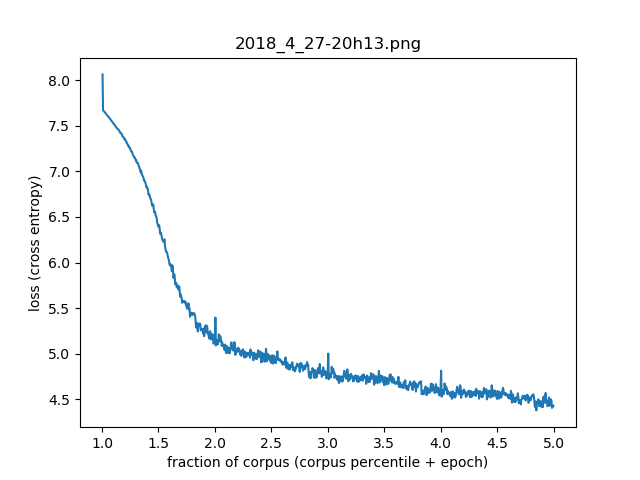
\includegraphics{parts/appendix/reports-gmsnn/docs_esteban-latex/test_reports/2018_4_27-20h13.png}
\caption{plot}
\end{figure}

\subsubsection{Details}

\begin{itemize}
\item
  log
  \href{https://gitlab.inria.fr/emarquer/awd-lstm-lm/blob/reimplement/logs/detrnn2018_4_27-14h11.log}{detrnn2018\_4\_27-14h11.log}
\item
  plot
  \href{https://gitlab.inria.fr/emarquer/awd-lstm-lm/blob/reimplement/plots/2018_4_27-20h13.png}{2018\_4\_27-16h42.png}
\end{itemize}

\subsection{Potential ameliorations \& next steps}

Next step is to test with more epochs, or test the growing model.

\end{report}
\begin{report}{Premier entraînement à 50 époques du modèle réimplémenté}\label{subsec:testreimp_3}
	% !TeX spellcheck = en_US
\section*{Test run of detrnn.py}

Test report

by E. Marquer, 2018/04/30, Synalp and Université de Lorraine

\subsection{Abstract}

Test to do a complete run on 50 epoch, with GPU, of the basic model of
DetRNN.

\subsection{Paradigm}

This test run of \emph{detrnn.py}, with INFO level log output, loss by
percentile and vbpc by epoch, will be executed with \emph{cuda}, for 50
epochs.

The test is done with branch
\href{https://gitlab.inria.fr/emarquer/awd-lstm-lm/tree/reimplement}{reimplement},
an allocated time of 76h, not interactive

Run time was estimated for 50 epochs according to the results for 4
epochs (see
\href{https://gitlab.inria.fr/emarquer/awd-lstm-lm/blob/master/docsEsteban/testReports/2018-04-27_test_run_detrnn.md}{2018-04-27\_test\_run\_detrnn.md}):

\begin{quote}
(5h 33min / 4 epoch) * 50 epoch = 4162.5min = 69h 22min 30s
\end{quote}

With a security margin of 10h, partially due to reduced batchsize, run
time is 80h.

\emph{/!\textbackslash{} Had to reduce batchsize down to 40 because of
memory errors /!\textbackslash{}}

\subsubsection{Node}

OAR\_JOB\_ID=155659 with GPU

Job start time: 2018-04-30 12:02:08

Estimated job stop time: 2018-05-03 16:02:08

Command used:
\lstinline!bash oarsub -q production -p "GPU <> 'NO'" -l "nodes=1,walltime=80:00:00" ~/awd-lstm-lm/rundet.sh!

\newpage
\subsection{Results}

Total run time for 50 epochs: with real stop time of 2018-05-02
17:16:56, the total run time of the training is aproximately 53h (2days
5h), corresponding to a little more than an hour per epoch.

BPC-wise, the DetRNN hardly goes under 2.7 even after 50 epoch, with a
change of 0.5 BPC in the last 30 epochs.

We can postulate that enven after 200 epoch, the DetRNN will not have a
BPC under 2.

\subsubsection{Plot}

\paragraph{BPC/fraction of corpus}

BPS per fraction of the corpus (an interval of 1 correspond a complete
corpus, or an epoch).

\begin{figure}[ht]
\centering
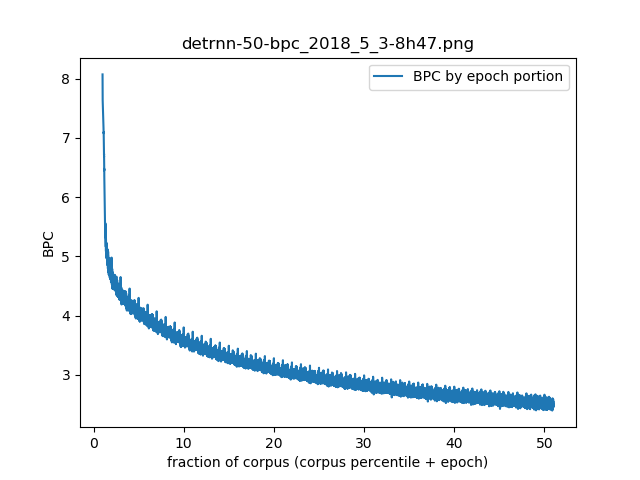
\includegraphics{parts/appendix/reports-gmsnn/docs_esteban-latex/test_reports/detrnn-50/detrnn-50-bpc_2018_5_3-8h47.png}
\caption{BPC}
\end{figure}

\newpage
\paragraph{ValBPC/epoch}

Mean BPC over the epoch, at the end of each epoch.

\begin{figure}[ht]
\centering
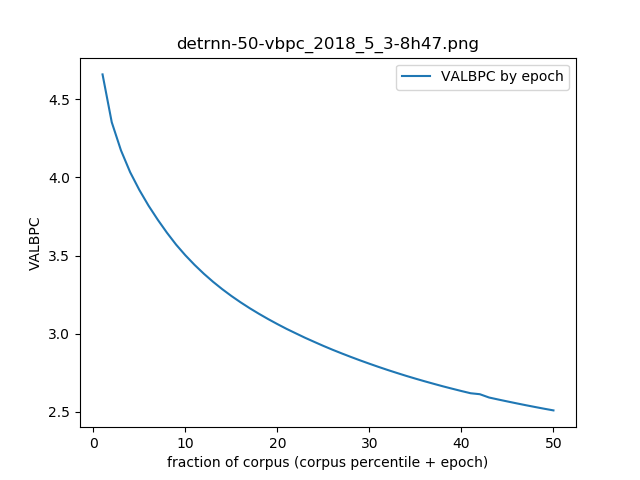
\includegraphics{parts/appendix/reports-gmsnn/docs_esteban-latex/test_reports/detrnn-50/detrnn-50-vbpc_2018_5_3-8h47.png}
\caption{ValBPC}
\end{figure}

\newpage
\paragraph{Loss}

Loss per fraction of the corpus (an interval of 1 correspond a complete
corpus, or an epoch).

\begin{figure}[ht]
\centering
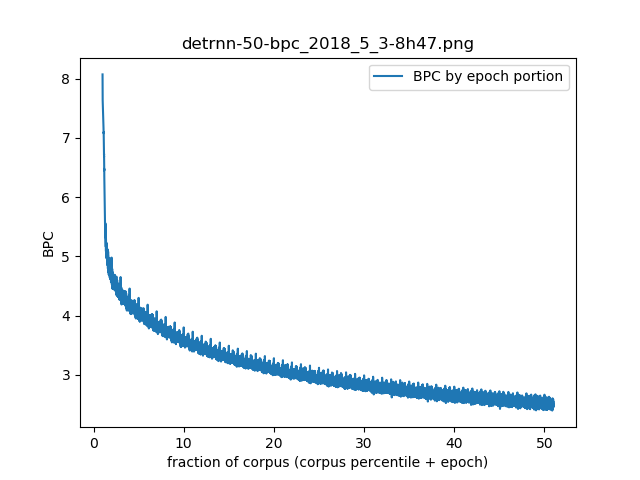
\includegraphics{parts/appendix/reports-gmsnn/docs_esteban-latex/test_reports/detrnn-50/detrnn-50-bpc_2018_5_3-8h47.png}
\caption{Loss}
\end{figure}

\subsubsection{Logs}

The log is available at 
\href{https://gitlab.inria.fr/emarquer/awd-lstm-lm/blob/reimplement/logs/detrnn-50_2018_4_30-12h2.log}{https://gitlab.inria.fr/emarquer/awd-lstm-lm/blob/reimplement/logs/detrnn-50\_2018\_4\_30-12h2.log}.

\subsection{Potential ameliorations \& next steps}

Next step is to test the growing model.

\end{report}
\begin{report}{Premier test du modèle multi-échelles}\label{subsec:testms}
	% !TeX spellcheck = en_US
\section*{Test run of detrnn.py}

Test report

by E. Marquer, 2018/05/03, Synalp and Université de Lorraine

\subsection{Abstract}

First performance test of the Test to do a run on 4 epochs, with GPU, of
the basic model of MSNN, with additive output strategy.

\subsection{Paradigm}

This test run of \emph{detrnn.py}, with DEBUG level log output, loss per
percentile and vbpc per epoch, that will be executed with \emph{cuda},
for 4 epochs.

The test is done with branch
\href{https://gitlab.inria.fr/emarquer/awd-lstm-lm/tree/growing}{growing},
an allocated time of 4h, not interactive.

Run time was estimated for 4 epochs according to a debug results for 0.2
epochs:

\begin{lstlisting}
(10min / 0.2 epoch) * 4 epoch = 200min = 3h 20min
\end{lstlisting}

With a security margin of 40min, run time is 4h.

\emph{/!\textbackslash{} Had to reduce batchsize down to 40 and halve
hidden size because of memoryerrors /!\textbackslash{}}

\newpage
\subsubsection{Hyperparameters}

\begin{longtable}[]{@{}ll@{}}
\hline
Hyperparameter & Value\tabularnewline
\hline
\endhead
nhidden & 920\tabularnewline
embedsize & 400\tabularnewline
bptt & 200\tabularnewline
batch\_size & 40\tabularnewline
eval\_batch\_size & 32\tabularnewline
lr & 0.001\tabularnewline
wdecay & 1.2e-06\tabularnewline
cuda\_on & True\tabularnewline
log\_interval & 20\tabularnewline
nepochs & 4\tabularnewline
max\_seqs & 15\tabularnewline
\hline
\end{longtable}

\subsubsection{Node}

OAR\_JOB\_ID=1558426 with GPU

Job start time: 2018-05-04 14:43:40

Estimated job stop time: 2018-05-04 18:43:40

Command used:

\begin{lstlisting}[language=bash]
oarsub -q production -p "GPU <> 'NO'" -l "nodes=1,walltime=04:00:00" ~/alt-repo/awd-lstm-lm/rundet.sh
\end{lstlisting}

Status verification loop:

\begin{lstlisting}[language=bash]
let x=0; while [ "true" ]; do echo "$x" $(oarstat -s -j 1558141); let ++x; sleep 120; done
\end{lstlisting}

\subsection{Results}

Total run time for 4 epochs: with real stop time of 2018-05-03 17:57:26,
the total run time of the training is aproximately 3h 13min,
corresponding to the predicted 50 min per epoch.

\newpage
\subsubsection{Comparative analysis}

With half the number of hidden parameters, and a yet unknown number of
layers, the basic MSNN has very similar results than the classical
DetRNN.

However, when analysing closely the learning speed, the MSNN seems to be
starting with a slower BPC decrease than the DetRNN, and it also seem to
be faster later on. Those variations are probably due to the number of
hidden layers.

\begin{figure}[h]
\centering
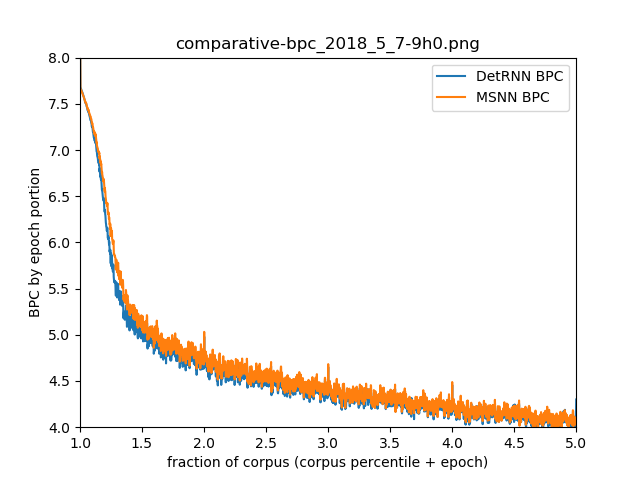
\includegraphics{parts/appendix/reports-gmsnn/docs_esteban-latex/test_reports/comparative-bpc-det-msnn_2018_5_7-9h0.png}
\caption{Comparative BPC}
\end{figure}

\subsubsection{Plot}

\paragraph{BPC/fraction of corpus}

BPS per fraction of the corpus (an interval of 1 correspond a complete
corpus, or an epoch).

\begin{figure}[h]
\centering
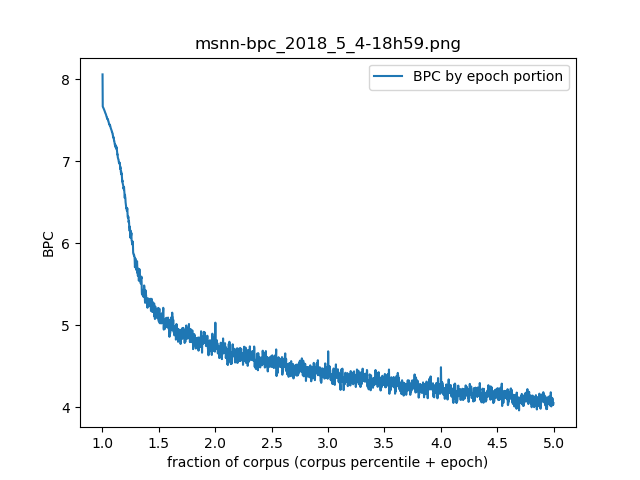
\includegraphics{parts/appendix/reports-gmsnn/docs_esteban-latex/test_reports/msnn-base/msnn-bpc_2018_5_4-18h59.png}
\caption{BPC}
\end{figure}

\paragraph{ValBPC/epoch}

Mean BPC over the epoch, at the end of each epoch.

\begin{figure}[h]
\centering
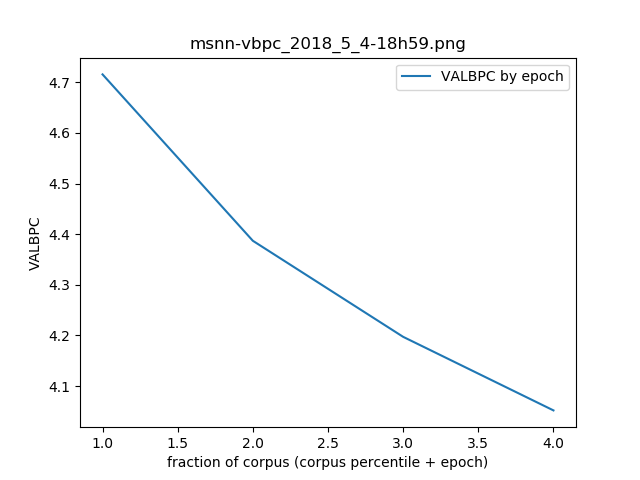
\includegraphics{parts/appendix/reports-gmsnn/docs_esteban-latex/test_reports/msnn-base/msnn-vbpc_2018_5_4-18h59.png}
\caption{ValBPC}
\end{figure}

\paragraph{Loss}

Loss per fraction of the corpus (an interval of 1 correspond a complete
corpus, or an epoch).

\begin{figure}[h]
\centering
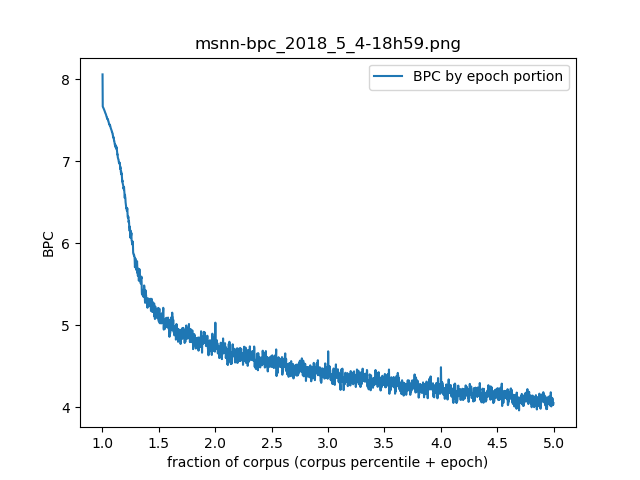
\includegraphics{parts/appendix/reports-gmsnn/docs_esteban-latex/test_reports/msnn-base/msnn-bpc_2018_5_4-18h59.png}
\caption{Loss}
\end{figure}

\subsubsection{Logs}

Reduced log is available at \href{msnn-base/msnn_2018_5_4-14h43.log}{msnn-base/msnn\_2018\_5\_4-14h43.log}.

\subsection{Potential ameliorations \& next steps}

A necessary amelioration is to add a way to track the number of layers.

As of now, the upper hidden layers participates in the output only when
updated. It is necessary to make them participate at every step.

The test process is not well defined: what to do when the eval batch is
dicontinuted from the training batch ? what if it is in the same corpus,
but not directly adjacent ? A possible yet hazardous solution would be
to evaluate a ``distance'' between the training and evaluation batches,
and reset the hidden states depending on that distance (a higher
distance would reset a higher number of layers).

Lastly, as the number of values to remember is increasing (bpc, loss,
layer number, \ldots{}) it would be interesting to improve the .plotdata
system.

Next step is to test the recurrently defined growing model.

\end{report}
\begin{report}{Comparaison des stratégies de fusion des résultats des différentes couches}\label{subsec:addcat}
	% !TeX spellcheck = en_US
\section*{Test run of detmsnn.py}

Test report

by E. Marquer, 2018/05/16, Synalp and Université de Lorraine

\subsection{Abstract}

Performance test of the `cat' (concatenated) output strategy compared to
the `add' strategy. Test to do a run on 4 epochs, with GPU, of the basic
model of MSNN, with concatenated output strategy.

\subsection{Paradigm}

This test run of \emph{detmsnn.py}, with INFO level log output, loss per
percentile and vbpc per epoch, is executed with \emph{cuda}, for 4
epochs.

The test is done with branch
\href{https://gitlab.inria.fr/emarquer/awd-lstm-lm/tree/growing}{growing},
an allocated time of 24h, not interactive

\textbf{/!\textbackslash{} Had to reduce evaluation courpus size down to
1/1000, to reduce computation time while keeping a big enough corpus to
compute BPC /!\textbackslash{}}

\newpage
\subsubsection{Hyperparameters}

\begin{longtable}[]{@{}ll@{}}
\hline
Hyperparameter & Value\tabularnewline
\hline
\endhead
nhidden & 920\tabularnewline
embedsize & 400\tabularnewline
bptt & 200\tabularnewline
batch\_size & 1\tabularnewline
eval\_batch\_size & 1\tabularnewline
lr & 0.001\tabularnewline
wdecay & 1.2e-06\tabularnewline
cuda\_on & True\tabularnewline
log\_interval & 100\tabularnewline
nepochs & 4\tabularnewline
max\_seqs & 5\tabularnewline
\hline
\end{longtable}

\subsubsection{Node}

OAR\_JOB\_ID=1563805 with GPU grimani-1

Job start time: 2018-05-16 08:53:20

Estimated job stop time: 2018-05-17 08:53:20

Command used:

\begin{lstlisting}[language=bash]
oarsub -q production -p "GPU <> 'NO'" -l "nodes=1,walltime=24:00:00" "bash runmsnn.sh"
\end{lstlisting}

Status verification loop:

\begin{lstlisting}[language=bash]
let x=0; while [ "true" ]; do echo "$x" $(oarstat -s -j 1563805); let ++x; sleep 120; done
\end{lstlisting}

\subsection{Results}

Total run time for 4 epochs: with real stop time of 08:53:28, the total
run time of the training is approximately 24h, with only 22\% of one
epoch done, and a final Validation BPC of 3.57.

Estimated run time for a full epoch: 24h / 22\% \textasciitilde{}=
109h/epoch. This corresponds to 436h for a 4 epoch run, and this is
critical.

The `cat' strategy is way more efficient in corpus consumption, even if
it is dramatically slower than the additive strategy.

\subsubsection{Comparative analysis}

The comparative plot shows that with the `cat' strategy, BPC diminution
is way faster than with the additive strategy. Computation-time wise, it
is obvious that the `cat' strategy is slower, with ??h/epoch, than the
`add' strategy, with 50min/epoch. This difference is too large to be due
to the device alone.

\begin{figure}[h]
\centering
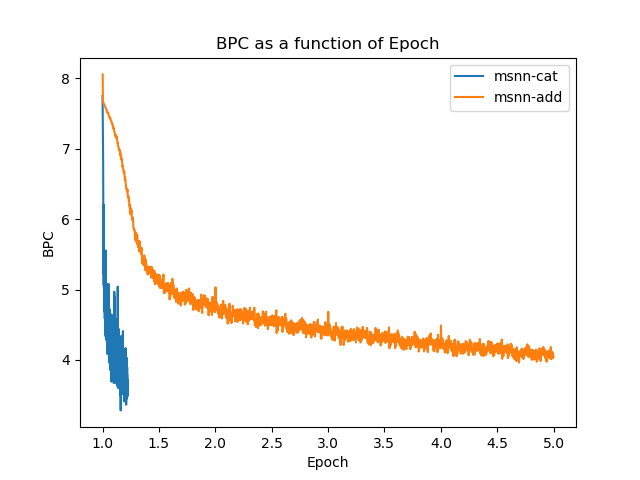
\includegraphics{parts/appendix/reports-gmsnn/docs_esteban-latex/test_reports/comparative-bpc-msnn-det-msnn-cat.png}
\caption{Comparative BPC}
\end{figure}

\subsubsection{Plot}

\paragraph{BPC/fraction of corpus}

BPC: BPC per fraction of the corpus (an interval of 1 correspond a
complete corpus, or an epoch).

Validation BPC: BPC per fraction of the corpus, on the validation
corpus.

Layers: Number of layers per fraction of the corpus.
\begin{figure}[h]
	\centering
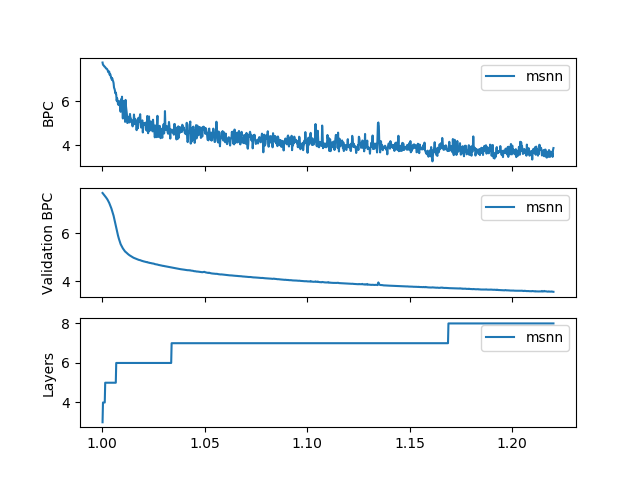
\includegraphics{parts/appendix/reports-gmsnn/docs_esteban-latex/test_reports/msnn-4/2018_05_17-13h49.png}
\caption{Comparative BPC}
\end{figure}

\newpage
\subsection{Potential ameliorations \& next steps}

Next step is to try to reduce run time.

\end{report}
\begin{report}{Test des effets du changement de taille des paquets (\foreign{batch})}\label{subsec:batch_1}
	% !TeX spellcheck = en_US
\section*{Test run of detmsnn.py}

Test report

by E. Marquer, 2018/05/16, Synalp and Université de Lorraine

\subsection{Abstract}

Performance test of batch size variation without deeper . Test to do a
run on 4 epochs, with GPU, of the basic model of MSNN, with concatenated
output strategy.

\subsection{Paradigm}

This test run of \emph{detmsnn.py}, with INFO level log output, loss per
percentile and vbpc per epoch, is executed with \emph{cuda}, for 4
epochs.

The test is done with branch
\href{https://gitlab.inria.fr/emarquer/awd-lstm-lm/tree/growing}{growing},
an allocated time of 24h, not interactive

\textbf{/!\textbackslash{} Had to reduce evaluation corpus size down to
1/1000, to reduce computation time while keeping a big enough corpus to
compute BPC /!\textbackslash{}}

\subsubsection{Hyperparameters}

\begin{longtable}[]{@{}ll@{}}
\hline
Hyperparameter & Value\tabularnewline
\hline
\endhead
nhidden & 920\tabularnewline
embedsize & 400\tabularnewline
bptt & 200\tabularnewline
batch\_size & 16\tabularnewline
lr & 0.001\tabularnewline
wdecay & 1.2e-06\tabularnewline
cuda\_on & True\tabularnewline
log\_interval & 100\tabularnewline
save\_interval & 100\tabularnewline
nepochs & 4\tabularnewline
max\_seqs & 5\tabularnewline
\hline
\end{longtable}

\subsubsection{Node}

OAR\_JOB\_ID=1567202 with GPU grimani-1

Planed job start time: 2018-05-19 02:41:08 Job start time: 2018-05-19
02:41:08

Estimated job stop time: 2018-05-22 14:41:08

Command used:

\begin{lstlisting}[language=bash]
oarsub -q production -p "GPU <> 'NO'" -l "nodes=1,walltime=84:00:00" "bash runmsnn.sh"
\end{lstlisting}

Status verification loop:

\begin{lstlisting}[language=bash]
let x=0; while [ "true" ]; do echo "$x" $(oarstat -s -j 1567202); let ++x; sleep 120; done
\end{lstlisting}

\subsection{Results}

Total run time for 4 epochs: with real stop time of ?, the total run
time of the training is approximately ?h, with only, and a final
Validation BPC of 3.57.

\subsubsection{Comparative analysis}

\textbf{NO PLOT HERE}

\subsubsection{Plot}

\paragraph{BPC/fraction of corpus}

BPC: BPC per fraction of the corpus (an interval of 1 correspond a
complete corpus, or an epoch).

Validation BPC: BPC per fraction of the corpus, on the validation
corpus.

Layers: Number of layers per fraction of the corpus. 

\textbf{NO PLOT HERE}

\subsection{Potential ameliorations \& next steps}

Next step is to continue run time reduction.

\end{report}


\begin{report}{Entraînement sur le corpus complet avec beaucoup de temps alloué}\label{subsec:long_train}
	% !TeX spellcheck = en_US
\section*{Long-run of RNN-MSNN}

Test report

by E. Marquer, 2018/05/29, Synalp and Université de Lorraine

\subsection{Abstract}

The run was done on the reduced enwik8 corpus.

The test is composed of 4 successive runs:
\begin{itemize}
	\item 1 run of 2h on grimani-4;
	\item 2 runs of 12h, both on grimani-1;
	\item 1 run of 50h on grele-11;
\end{itemize}

End causes are as follow: 
\begin{itemize}
	\item Run 1: out of time (2h);
	\item Run 2: out of time (12h);
	\item Run 3: end of epoch crash (7h30);
	\item Run 4: end of epoch crash (19h15);
\end{itemize}

Mean time for an epoch is about 19h 15min (on the reduced version of the
corpus). Two epochs were completed.

\subsection{Results}

Each run crashed between epochs, so a bit of patching had to be made on
top of fixing the bug.

\subsubsection{Memory}

Both RAM and video RAM are still subject to a constant leak in memory.
But even if it does not show on the plots (scale is too small), logs
confirm that there is no leak during validation.

\begin{figure}[H]
\centering
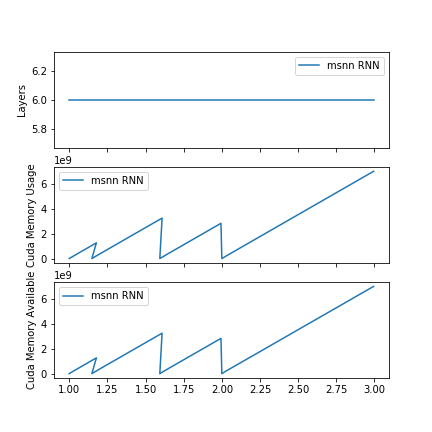
\includegraphics{parts/appendix/reports-gmsnn/docs_esteban-latex/test_reports/2018-06-11/memory.png}
\caption{Memory usage}
\end{figure}

\begin{figure}[H]
\centering
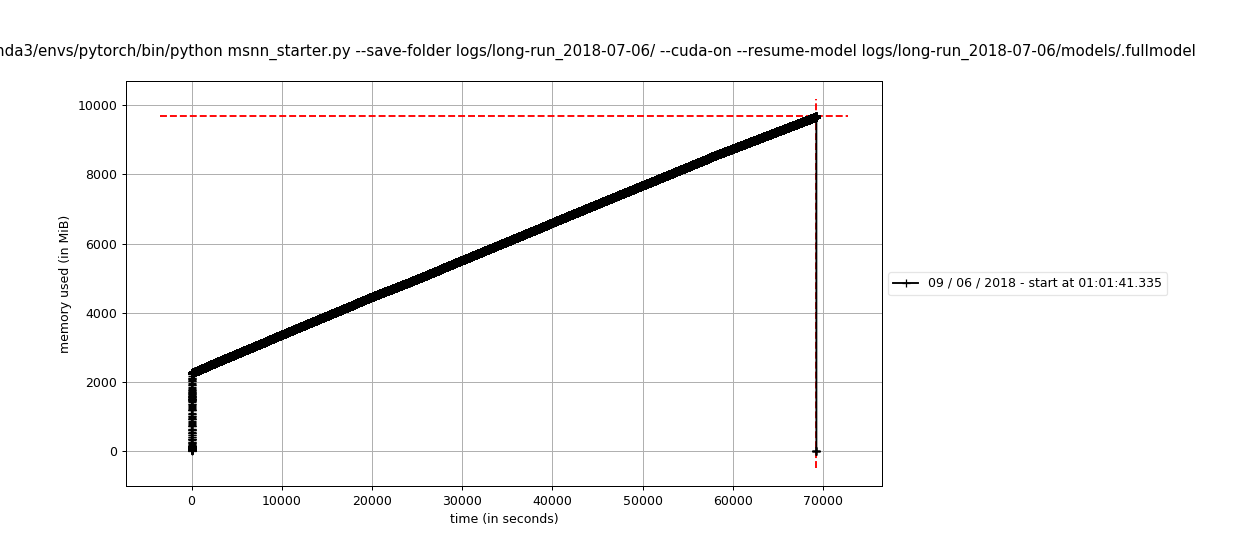
\includegraphics[width=\textwidth]{parts/appendix/reports-gmsnn/docs_esteban-latex/test_reports/2018-06-11/RAM_restart-2.png}
\caption{RAM third run}
\end{figure}

An other noticeable property is that ``Run Time'', corresponding to the
time to train over \emph{log\_interval} sequences, is mostly
proportional to CUDA memory usage. The source of the cuda memory leak is
probably the same as what makes training slower.

\begin{figure}[H]
\centering
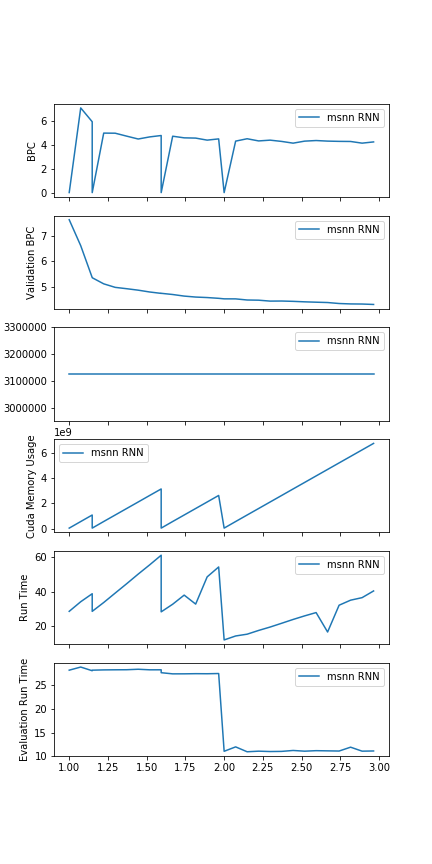
\includegraphics[height=.8\textheight]{parts/appendix/reports-gmsnn/docs_esteban-latex/test_reports/2018-06-11/frac.png}
\caption{Memory and computation time}
\end{figure}

\newpage
\subsubsection{BPC / Validation BPC}

BPC and Validation BPC

\begin{figure}[H]
\centering
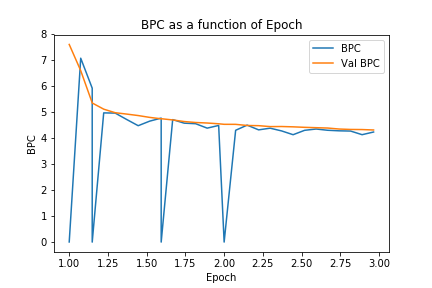
\includegraphics[width=\textwidth]{parts/appendix/reports-gmsnn/docs_esteban-latex/test_reports/2018-06-11/frac_val_bpc.png}
\caption{BPC}
\end{figure}


\newpage
\subsubsection{Job restart}\label{job-restart}

When resuming a job, CUDA memory is entirely freed. Same thing can be
said about RAM.

\begin{figure}[H]
\centering
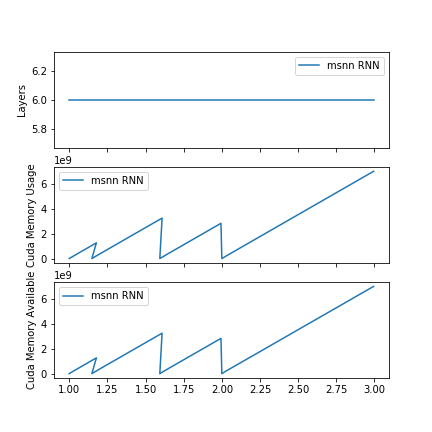
\includegraphics[width=\textwidth]{parts/appendix/reports-gmsnn/docs_esteban-latex/test_reports/2018-06-11/memory.png}
\caption{Memory usage}
\end{figure}

\begin{figure}[H]
\centering
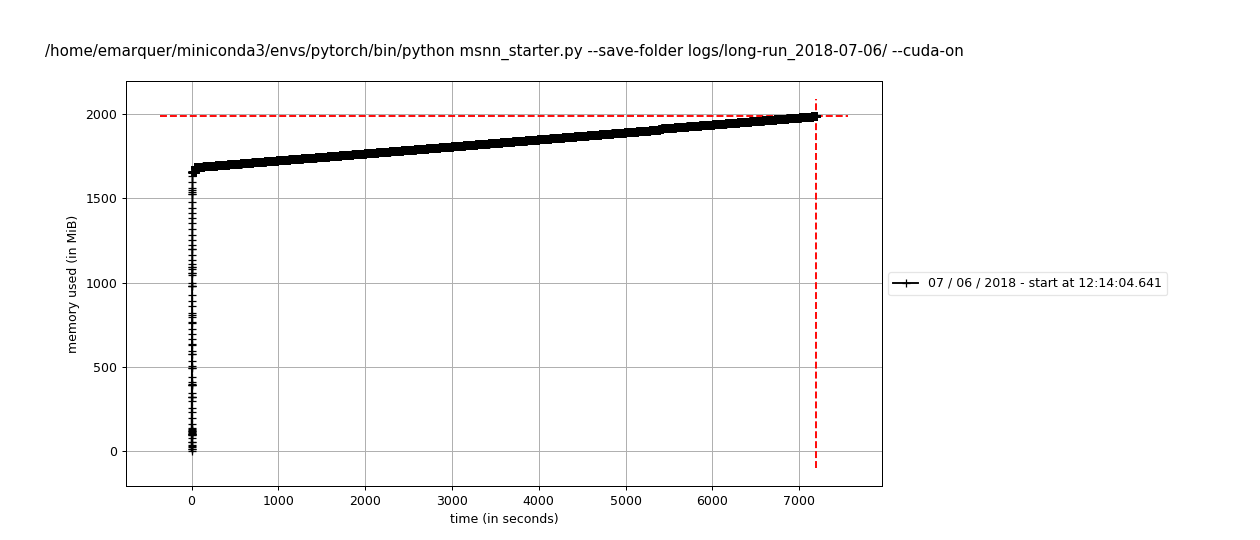
\includegraphics[width=\textwidth]{parts/appendix/reports-gmsnn/docs_esteban-latex/test_reports/2018-06-11/RAM.png}
\caption{RAM first run}
\end{figure}

\begin{figure}[H]
\centering
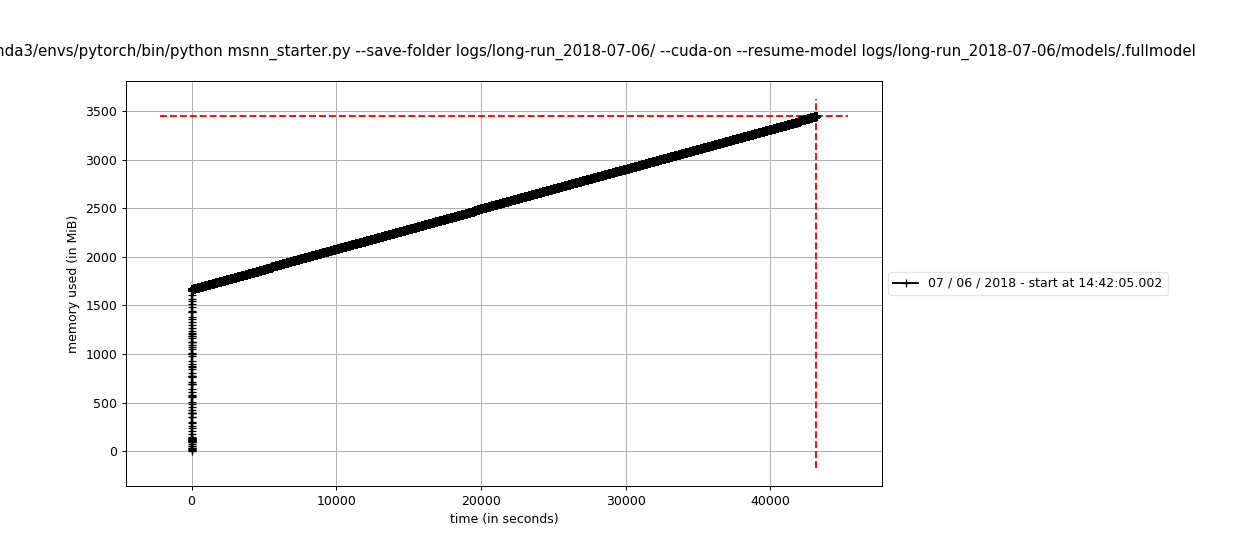
\includegraphics[width=\textwidth]{parts/appendix/reports-gmsnn/docs_esteban-latex/test_reports/2018-06-11/RAM_restart-1.png}
\caption{RAM second run}
\end{figure}

\begin{figure}[H]
\centering
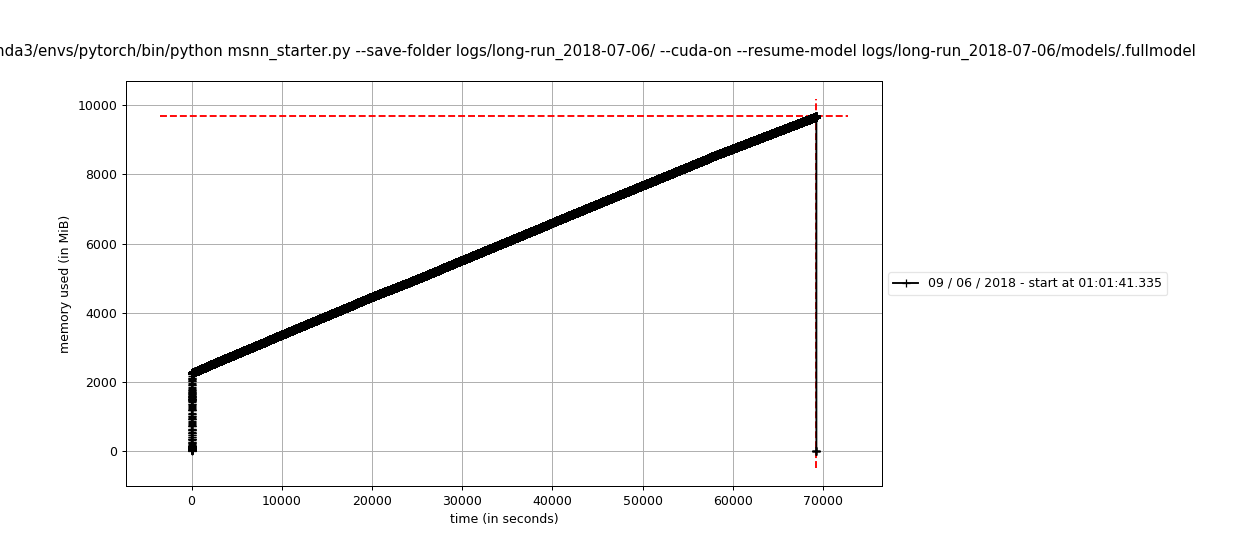
\includegraphics[width=\textwidth]{parts/appendix/reports-gmsnn/docs_esteban-latex/test_reports/2018-06-11/RAM_restart-2.png}
\caption{RAM third run}
\end{figure}

Memory is freed each time the job is restarted, meaning either a part of
the necessary is discarded, or unnecessary data is kept in memory. As in
CUDAles tests a memory maximum was reached, CUDA seems to be the source
of the leak (data copies not removed, \ldots{}).

\subsection{Next steps}

Debug end of epoch bug. Try to patch memory leak. Continue training.

\end{report}
\begin{report}{Changement de stratégie de gestion d'historique}\label{subsec:change_history}
	\section*{Change history}

Analysis report

by E. Marquer, 2018/06/12, Synalp and Université de Lorraine

\subsection{Abstract}

As computation graph has been confirmed to exist/be considered only in
the last history, keeping an explicit history is no longer necessary.
Worst, it may hinder garbage collection, by keeping references to
Tensors that are completely useless.

A new model of history has been made to keep only a reference to the
last hidden state. This new model will be referred as ``last'', and the
old one keeping an explicit history as ``classical''.

\subsection{Tests}

Multiple tests were done on the new ``enwik8mini'' corpus of 100,000 characters:
\begin{itemize}
\item ``last'' a test run on 2 epochs with 1 batches of ``last'' history
\item ``last b2'' a test run on 10 epochs with 2 batches of ``last'' history
\item ``last b2 10epoch'' a test run on 10 epochs with 2 batches of ``last'' history
\item ``classical'' a test run on 2 epochs with 1 batches of ``classical'' history
\end{itemize}

\subsubsection{Results (1 epoch)}

The results are over 1 epoch, with values from the start of the first
and the second epoch. As ``last b2 10epoch'' and ``last b2'' have the
same set of parameters, they coincides.

\begin{figure}[h]
\centering
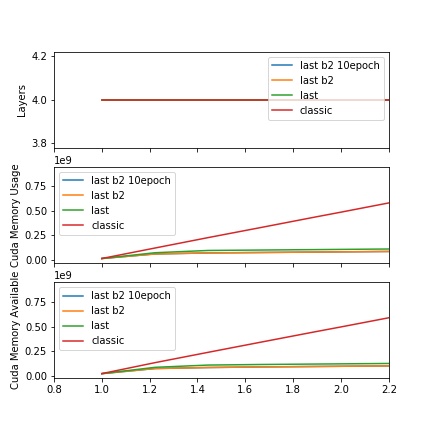
\includegraphics{parts/appendix/reports-gmsnn/docs_esteban-latex/test_reports/2018-06-12/history_memory_1e.png}
\caption{Memory 1 epoch}
\end{figure}

\begin{figure}[h]
\centering
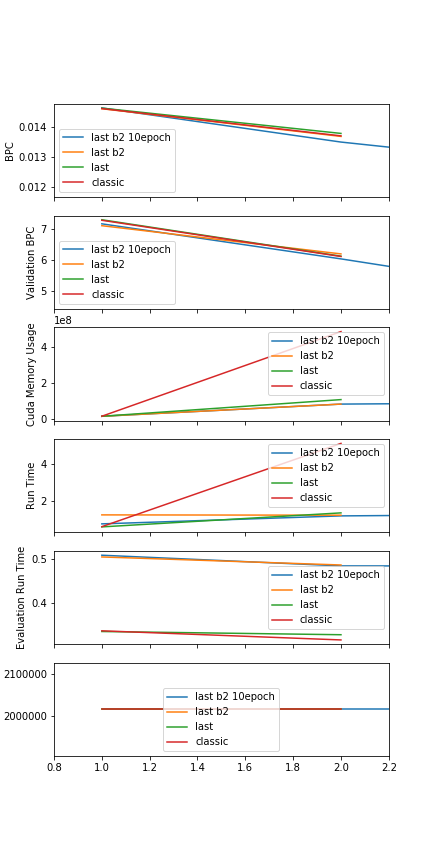
\includegraphics{parts/appendix/reports-gmsnn/docs_esteban-latex/test_reports/2018-06-12/history_frac_1e.png}
\caption{All info 1 epoch}
\end{figure}

\subsubsection{Results (full)}

\begin{figure}[h]
\centering
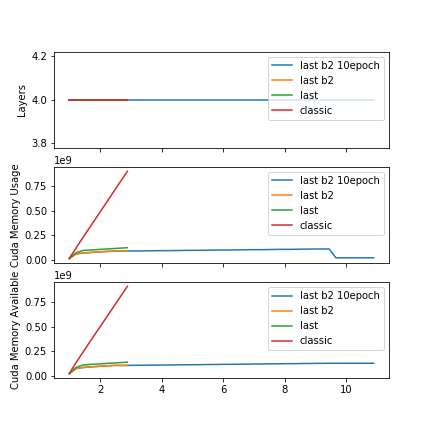
\includegraphics{parts/appendix/reports-gmsnn/docs_esteban-latex/test_reports/2018-06-12/history_memory.png}
\caption{Memory}
\end{figure}

\begin{figure}[h]
\centering
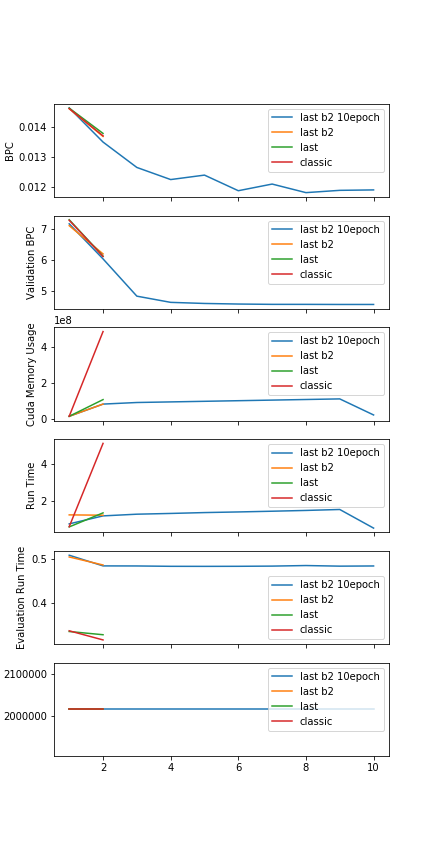
\includegraphics{parts/appendix/reports-gmsnn/docs_esteban-latex/test_reports/2018-06-12/history_frac.png}
\caption{All info}
\end{figure}

\paragraph{\texorpdfstring{Ram consumption for ``last b2 10epoch''}{Ram consumption for last b2 10epoch}}

\begin{figure}[h]
\centering
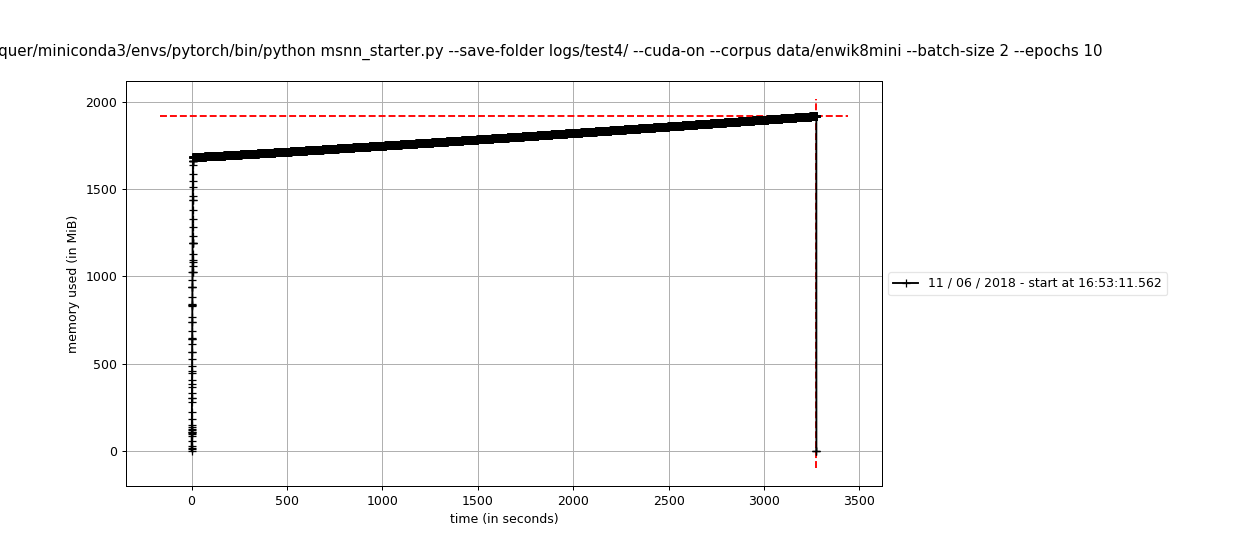
\includegraphics{parts/appendix/reports-gmsnn/docs_esteban-latex/test_reports/2018-06-12/history_RAM.png}
\caption{RAM 10 epoch}
\end{figure}

\subsection{Conclusion}

\subsubsection{Memory leak}

The leak in CUDA memory has reduced drastically.

It seems there is still a leak, this leak is not present when CUDA is
not used. This leak is present in both RAM and graphical RAM, but the
remaining leak in graphical RAM is not a concern anymore, with only a
dozen MiB over 1,000,000 characters (10 epochs * 100,000 characters).
However, the leak in RAM has not reduced, and even if it is not a
problem thanks to the available RAM in the cluster, it would be
preferable to identify the source of the leak.

\subsubsection{Run (training) time}

Additionally, the correlation of CUDA memory usage and and training run
time is kept, so the small remaining CUDA leak is probably linked to the
computation graph. With CUDA memory usage drastically reduced, run time
has been reduced too.

Currently, training over 100,000 characters (with 2 batches) only takes
5 minutes.

\subsubsection{Performances}

No conclusion can be drawn on learning performances, due to the size of
the learning corpus. Even though, it is encouraging that even with a
small corpus 10 epochs are not enough to have over-fitting (at least
with 2 batches).

\subsection{Next steps}

\begin{enumerate}
\def\labelenumi{\arabic{enumi}.}
\item
  long training over the ``enwik8reduced'' or the ``enwik8'' corpus;
\item
  fix (or at least identify) RAM leak
\end{enumerate}

\end{report}
\begin{report}{Test de l'implémentation des \foreign{batchs}}\label{subsec:test_batch}\label{subsec:batch_2}
	\section*{Long-run of RNN-MSNN}

Test report

by E. Marquer, 2018/06/13 Synalp and Université de Lorraine

\subsection{Abstract}

The test is composed of 2 successive runs:
\begin{itemize}
\item id 1582586: batch-size 1, bptt 200 on grele-4;
\item id 1582587: batch-size 2, bptt 100 on grimani-6.
\end{itemize}

Run time is about 10h in each case, corresponding to 2h30 for an epoch.
In both case corpus batches rotation over epochs was disabled.

\subsubsection{Shared parameters}

\begin{longtable}[]{@{}ll@{}}
\hline
parameter & value\tabularnewline
\hline
\endhead
corpus & enwik8reduced\tabularnewline
history\_strategy & layer-constant-length\tabularnewline
max\_history & 25\tabularnewline
bptt & \emph{variable}\tabularnewline
batch\_size & \emph{variable}\tabularnewline
epochs & 4\tabularnewline
lr & 1e-3\tabularnewline
weight\_decay & 1.2e-6\tabularnewline
epochs & 4\tabularnewline
valid\_len & 500,000\tabularnewline
log\_interval & 500\tabularnewline
save\_interval & 500\tabularnewline
memory\_interval & 100\tabularnewline
hidden\_size & 460\tabularnewline
embed\_size & 400\tabularnewline
growth\_factor & 5\tabularnewline
rnn\_type & RNN\tabularnewline
reset\_hidden & False\tabularnewline
reset\_growth & True\tabularnewline
cuda\_on & True\tabularnewline
\hline
\end{longtable}

\subsection{Results}

At the end of each epoch, we see a spike in BPC, due to the first
evaluation of the epoch. As corpus rotation is disabled, it is not
surprising that with two batches over-fitting appears.

Moreover, we can note that run time is constant and memory usage tend to
a constant value (1.6 GiB), with no difference between 1 and 2 batches.
Note: the product \lstinline!bptt * batch_size! is equal for 1 and 2
batches, so this result is the one predicted by the equations.

\begin{figure}[h]
\centering
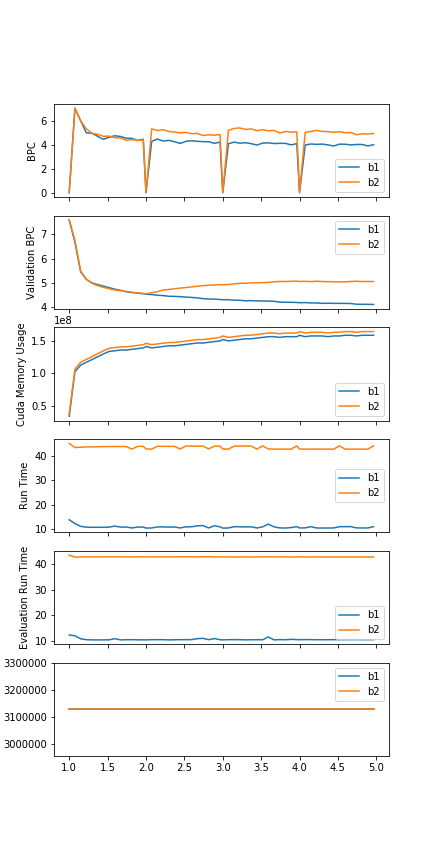
\includegraphics{parts/appendix/reports-gmsnn/docs_esteban-latex/test_reports/2018-06-13/batch_1_2_frac.png}
\caption{RAM third run}
\end{figure}

\begin{figure}[h]
\centering
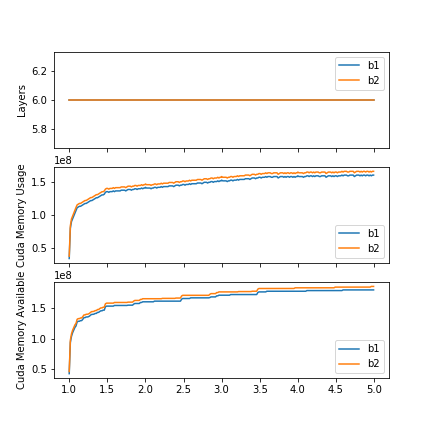
\includegraphics{parts/appendix/reports-gmsnn/docs_esteban-latex/test_reports/2018-06-13/batch_1_2_memory.png}
\caption{Memory usage}
\end{figure}

\subsection{Next steps}

\begin{itemize}
\item
  batches:

  \begin{enumerate}
  \def\labelenumi{\arabic{enumi}.}
  \item
    Implement corpus rotation
  \item
    See if corpus rotation solves over-fitting
  \item
    Compare run time on comparable machines
  \end{enumerate}
\item
  long run:

  \begin{enumerate}
  \def\labelenumi{\arabic{enumi}.}
  \item
    Continue batch 1 for more epochs
  \item
    See when over-fitting appears
  \end{enumerate}
\end{itemize}

\end{report}
\begin{report}{Test des performances des \foreign{batchs}}\label{subsec:test_batch_perf}\label{subsec:batch_3}
	\section{Run on the same node of RNN-MSNN with different batch
size}\label{run-on-the-same-node-of-rnn-msnn-with-different-batch-size}

Test report

by E. Marquer, 2018/06/15 Synalp and Université de Lorraine

\subsection{Abstract}\label{abstract}

The test is composed of 2 runs: - id 1583339: batch-size 1, bptt 200 on
grele-2 - id 1583336: batch-size 2, bptt 100 on grele-1

Run time per epoch varies from 28 to 20 min for a single batch and from
20 to 11 min for two batches.

\subsubsection{Shared parameters}\label{shared-parameters}

\begin{longtable}[]{@{}ll@{}}
\toprule
parameter & value\tabularnewline
\midrule
\endhead
corpus & enwik8reduced\tabularnewline
history\_strategy & layer-constant-length\tabularnewline
max\_history & 25\tabularnewline
bptt & \emph{variable}\tabularnewline
batch\_size & \emph{variable}\tabularnewline
epochs & 4\tabularnewline
lr & 1e-3\tabularnewline
weight\_decay & 1.2e-6\tabularnewline
epochs & 4\tabularnewline
valid\_len & 500,000\tabularnewline
log\_interval & 500\tabularnewline
save\_interval & 500\tabularnewline
memory\_interval & 100\tabularnewline
hidden\_size & 460\tabularnewline
embed\_size & 400\tabularnewline
growth\_factor & 5\tabularnewline
rnn\_type & RNN\tabularnewline
reset\_hidden & False\tabularnewline
reset\_growth & True\tabularnewline
cuda\_on & True\tabularnewline
\bottomrule
\end{longtable}

\subsection{Results}\label{results}

At the end of each epoch, we see a spike in BPC, due to the first
evaluation of the epoch (BPC is reinitialised to 0, causing a spike).
With 2 btches, BPC is also more stable.

As of now, run time is computed after running validation, so training
time is \lstinline!real_training_time = run_time - validation_time!. But
validation time increase with the number of batches as the number of
characters seen increase (the whole validation corpus is used for each
batch, so the number of characters seen during validation is
\lstinline!validation_corpus_len * batches!). That explains that the
evaluation time for a batch is lower than for 2 batches.

By removing evaluation time, we can obtain a reasonable and coherent
(with regard to epoch run time) estimation of training time over a
sequence.

\subsubsection{Epoch run time:}\label{epoch-run-time}

\begin{longtable}[]{@{}lll@{}}
\toprule
Epoch & Run time b=1 & Run time b=2\tabularnewline
\midrule
\endhead
1 & 28 min & 20 min\tabularnewline
2 & 23 min & 17 min\tabularnewline
3 & 22 min & 14 min\tabularnewline
4 & 20 min & 11 min\tabularnewline
\bottomrule
\end{longtable}

There is a notable decrease in epoch run time (time necessary to run
over an epoch), of about 10 min over the 4 epochs, with both runs.

Possible causes for the decrease of run time: - part of the graph is
already computed, and this part is skipped; - corpus data is already
loaded in cuda memory.

Both of them are highly unlikely to cause such a decrease. A more
precise training time storage may provide an explanation.

\subsubsection{Plots}\label{plots}

\begin{figure}
\centering
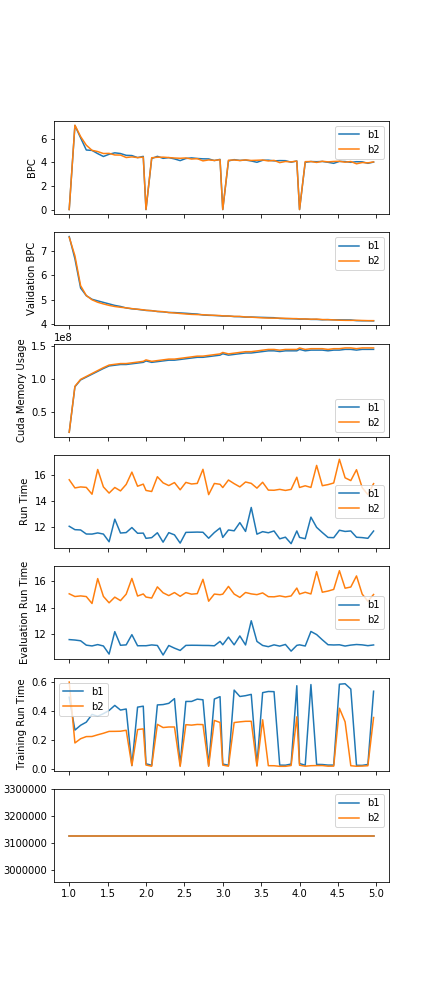
\includegraphics{2018_06_15_frac.png}
\caption{Full data}
\end{figure}

\begin{figure}
\centering
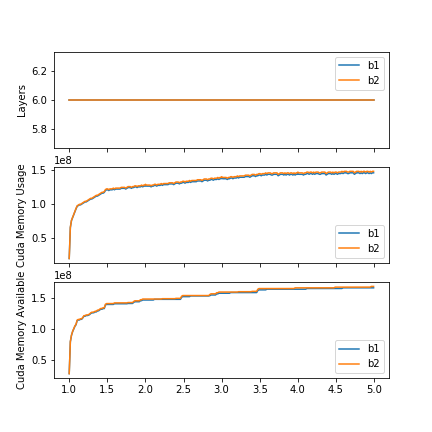
\includegraphics{2018_06_15_memory.png}
\caption{Memory usage}
\end{figure}

\subsection{Next steps}\label{next-steps}

\begin{itemize}
\tightlist
\item
  Data

  \begin{itemize}
  \tightlist
  \item
    Implement more precise time data saving (epoch run time and training
    run time)
  \end{itemize}
\item
  Runs (objective: 100 epochs)

  \begin{itemize}
  \tightlist
  \item
    Continue running batches 1 and 2
  \item
    Try with higher number of batches
  \end{itemize}
\item
  {[}Optional{]} Other experimental branch

  \begin{enumerate}
  \def\labelenumi{\arabic{enumi}.}
  \tightlist
  \item
    Implement prepared attention module in every layer
  \item
    Analyse results
  \item
    Patch probable memory leaks
  \end{enumerate}
\end{itemize}

\end{report}
\begin{report}{Test des performances des \foreign{batchs} sur 50 époques}\label{subsec:test_batch_perf_}\label{subsec:batch_4}
	\section{Run over more than 50 epochs with varied batch
size}\label{run-over-more-than-50-epochs-with-varied-batch-size}

Test report

by E. Marquer, 2018/06/19 Synalp and Université de Lorraine

\subsection{Abstract}\label{abstract}

The test is composed of 4 runs on grele, with: - bptt 200, batch-size 1
- bptt 100, batch-size 2 - bptt 50, batch-size 4 - bptt 25, batch-size 8

Run has been interrupted by an overflow of disk space due to the
detailed logs; next runs will used reduced logs.

Run time per epoch varies from 30 to 7 min.

\subsubsection{Shared parameters}\label{shared-parameters}

\begin{longtable}[]{@{}ll@{}}
\toprule
parameter & value\tabularnewline
\midrule
\endhead
corpus & enwik8reduced\tabularnewline
history\_strategy & layer-constant-length\tabularnewline
max\_history & 25\tabularnewline
bptt & \emph{variable}\tabularnewline
batch\_size & \emph{variable}\tabularnewline
epochs & 4\tabularnewline
lr & 1e-3\tabularnewline
weight\_decay & 1.2e-6\tabularnewline
epochs & 4\tabularnewline
valid\_len & 500,000\tabularnewline
log\_interval & 500\tabularnewline
save\_interval & 500\tabularnewline
memory\_interval & 100\tabularnewline
hidden\_size & 460\tabularnewline
embed\_size & 400\tabularnewline
growth\_factor & 5\tabularnewline
rnn\_type & RNN\tabularnewline
reset\_hidden & False\tabularnewline
reset\_growth & True\tabularnewline
cuda\_on & True\tabularnewline
\bottomrule
\end{longtable}

\subsection{Results}\label{results}

At the end of each epoch, we see a spike in BPC, due to the first
evaluation of the epoch (BPC is reinitialised to 0, causing a spike).
With any number of batch, while keeping the
\lstinline!bptt * batch_size! ratio, BPC and Validation BPC do not vary.

Even with 200 epochs, with batch size of 1, there is no trace of
over-fitting.

\subsubsection{Epoch run time:}\label{epoch-run-time}

\begin{longtable}[]{@{}lllll@{}}
\toprule
Epoch & Run time b=1 & Run time b=2 & Run time b=4 & Run time
b=8\tabularnewline
\midrule
\endhead
1 & 30 min & 21 min & 18 min & 19 min\tabularnewline
10 & 21 min & 14 min & 14 min & 17 min\tabularnewline
\textgreater{}15 & 7 min & 7 min & 8 min & 11 min\tabularnewline
\bottomrule
\end{longtable}

\begin{longtable}[]{@{}lll@{}}
\toprule
Epoch 1 & Epoch 10 & Epoch 15\tabularnewline
\midrule
\endhead
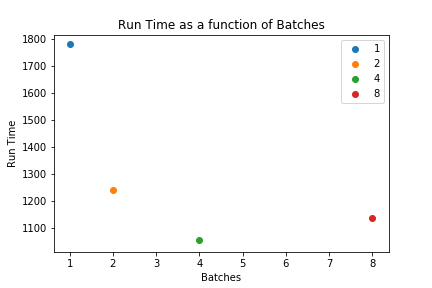
\includegraphics{b1a8_batch_epoch_1.png} &
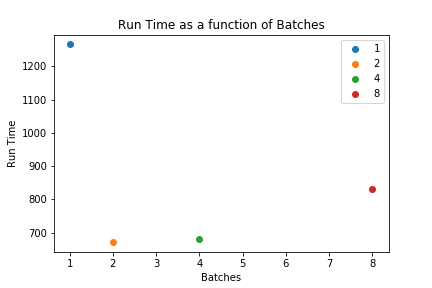
\includegraphics{b1a8_batch_epoch_10.png} &
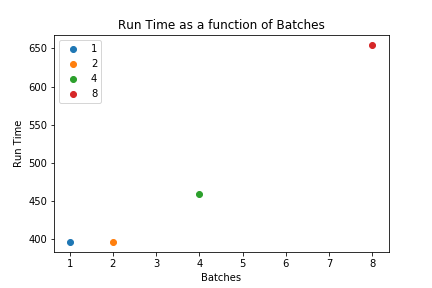
\includegraphics{b1a8_batch_epoch_15.png}\tabularnewline
\bottomrule
\end{longtable}

Run time can be split over two set of epochs: before, and after the 15th
epoch. Before the 15th epoch, run is faster with more batches, with the
exception of batch-size 8, which is slower than batch-size 2 and 4.
After the 15th epoch, run is slower with more batches.

To optimize run time, it is necessary to balance run time before 15
epochs. If a high number of batches is planed (\textgreater{}50),
between 2 and 4 batches are preferable, because the run time after epoch
15 has a lot of impact on global run time; however, if only a few epochs
are planed (\textless{}20), a high number of batches is preferable, as
run time before epoch 15 is the most important.

With current corpus, 2, 3 or 4 batches are the most interesting setup.

Decrease in run time is most probably due to the history of the upper
layers, that needs multiple epochs to fill.

\subsubsection{Plots}\label{plots}

\paragraph{BPC}\label{bpc}

\begin{figure}
\centering
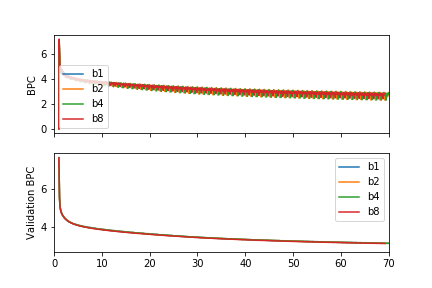
\includegraphics{b1a8_frac.png}
\caption{Full data}
\end{figure}

\begin{figure}
\centering
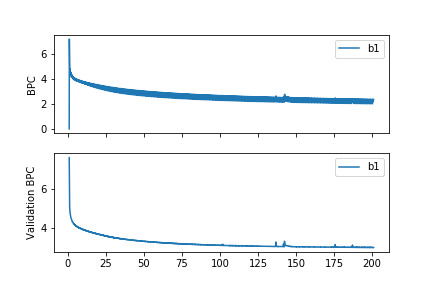
\includegraphics{b1a8_200.png}
\caption{Full data}
\end{figure}

\paragraph{Memory}\label{memory}

\begin{figure}
\centering
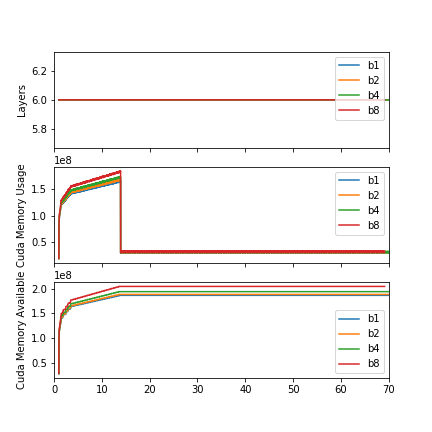
\includegraphics{b1a8_memory.png}
\caption{Full data}
\end{figure}

\paragraph{Run time (in seconds)}\label{run-time-in-seconds}

\begin{figure}
\centering
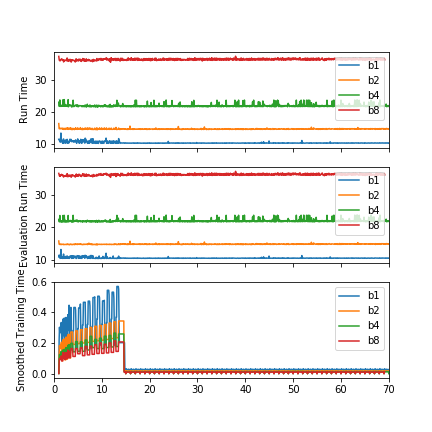
\includegraphics{b1a8_time.png}
\caption{Run time}
\end{figure}

\subparagraph{Epoch run time}\label{epoch-run-time-1}

\begin{figure}
\centering
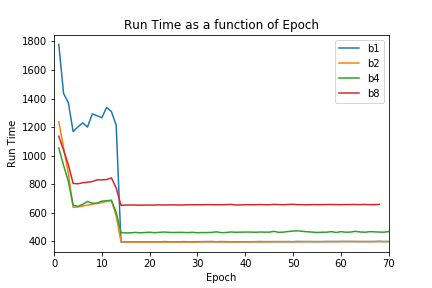
\includegraphics{b1a8_epoch.png}
\caption{Epoch run time}
\end{figure}

\subsection{Next steps}\label{next-steps}

\begin{itemize}
\tightlist
\item
  Independent impact of batch number and sequence length:

  \begin{itemize}
  \tightlist
  \item
    Run with fixed batch number and varying sequence length
  \item
    Run with fixed sequence length and varying batch number
  \end{itemize}
\item
  Impact of corpus length on optimal number of batch and sequences:

  \begin{itemize}
  \tightlist
  \item
    Run with varying sequence length and varying batch number over the
    full length corpus
  \end{itemize}
\item
  Number of parameters:

  \begin{itemize}
  \tightlist
  \item
    Increase the hidden layer size
  \end{itemize}
\item
  {[}Future{]} Transmission rate impact:

  \begin{itemize}
  \tightlist
  \item
    Compare optimal values of parameters, and BPC reached with varying
    transmission rate
  \end{itemize}
\end{itemize}

\end{report}
\begin{report}{Test des performances des différentes améliorations}\label{subsec:test_perf}
	\section{Run over more than 50 epochs with varied batch
size}\label{run-over-more-than-50-epochs-with-varied-batch-size}

Test report

by E. Marquer, 2018/06/19 Synalp and Université de Lorraine

\subsection{Abstract}\label{abstract}

The test runs are for two parallel experiments: - test which of 2 and 3
batches are the most interesting - test the impact of layer by layer
training (with an intuitive algorithm developed out of work-time)

The test is composed of 4 runs on grele, with: - bptt 200/2, batch-size
2 - bptt 200/3, batch-size 3 - bptt 200/2, batch-size 2, layer by layer
training, - bptt 200/2, batch-size 2, layer by layer training, 20 epochs
of individual training for each layer, 10 epochs of common fine-tuning
for already trained layers (see below the explanation of this algorithm)

\subsubsection{Shared parameters}\label{shared-parameters}

\begin{longtable}[]{@{}ll@{}}
\toprule
parameter & value\tabularnewline
\midrule
\endhead
corpus & enwik8reduced\tabularnewline
history\_strategy & last\tabularnewline
max\_history & 25\tabularnewline
lr & 1e-3\tabularnewline
weight\_decay & 1.2e-6\tabularnewline
epochs & 1500\tabularnewline
valid\_len & 500,000\tabularnewline
log\_interval & 500\tabularnewline
save\_interval & 500\tabularnewline
memory\_interval & 100\tabularnewline
hidden\_size & 460\tabularnewline
embed\_size & 400\tabularnewline
growth\_factor & 5\tabularnewline
rnn\_type & RNN\tabularnewline
reset\_hidden & False\tabularnewline
reset\_growth & True\tabularnewline
cuda\_on & True\tabularnewline
\bottomrule
\end{longtable}

\subsubsection{Model keys and
specificities}\label{model-keys-and-specificities}

When noting is specified, all models have:

\begin{itemize}
\tightlist
\item
  2 batches, and a sequence length of 200/2
\item
  1 RNN layer per MSNN layer
\end{itemize}

\begin{longtable}[]{@{}ll@{}}
\toprule
\begin{minipage}[b]{0.08\columnwidth}\raggedright\strut
Model\strut
\end{minipage} & \begin{minipage}[b]{0.86\columnwidth}\raggedright\strut
Specificity\strut
\end{minipage}\tabularnewline
\midrule
\endhead
\begin{minipage}[t]{0.08\columnwidth}\raggedright\strut
b2\strut
\end{minipage} & \begin{minipage}[t]{0.86\columnwidth}\raggedright\strut
classical model, comparison basis\strut
\end{minipage}\tabularnewline
\begin{minipage}[t]{0.08\columnwidth}\raggedright\strut
b3\strut
\end{minipage} & \begin{minipage}[t]{0.86\columnwidth}\raggedright\strut
3 batches, sequence length of 200/3\strut
\end{minipage}\tabularnewline
\begin{minipage}[t]{0.08\columnwidth}\raggedright\strut
s\strut
\end{minipage} & \begin{minipage}[t]{0.86\columnwidth}\raggedright\strut
``scheduled(10,10)'': use layer by layer training; 10 epochs for
individual training, 10 epochs for intermediary fine-tuning\strut
\end{minipage}\tabularnewline
\begin{minipage}[t]{0.08\columnwidth}\raggedright\strut
s-a20-l10\strut
\end{minipage} & \begin{minipage}[t]{0.86\columnwidth}\raggedright\strut
``scheduled(20,10)'': use layer by layer training; 20 epochs for
individual training, 10 epochs for intermediary fine-tuning\strut
\end{minipage}\tabularnewline
\begin{minipage}[t]{0.08\columnwidth}\raggedright\strut
l2\strut
\end{minipage} & \begin{minipage}[t]{0.86\columnwidth}\raggedright\strut
2 RNN layer per MSNN layer\strut
\end{minipage}\tabularnewline
\begin{minipage}[t]{0.08\columnwidth}\raggedright\strut
l3\strut
\end{minipage} & \begin{minipage}[t]{0.86\columnwidth}\raggedright\strut
3 RNN layer per MSNN layer\strut
\end{minipage}\tabularnewline
\begin{minipage}[t]{0.08\columnwidth}\raggedright\strut
s\_l3\_a\strut
\end{minipage} & \begin{minipage}[t]{0.86\columnwidth}\raggedright\strut
3 RNN layer per MSNN layer, ``scheduled(10,10)'' (see model ``s''),
attentive intermediary input\strut
\end{minipage}\tabularnewline
\bottomrule
\end{longtable}

\subsubsection{Series}\label{series}

\begin{longtable}[]{@{}llll@{}}
\toprule
\begin{minipage}[b]{0.04\columnwidth}\raggedright\strut
Series\strut
\end{minipage} & \begin{minipage}[b]{0.08\columnwidth}\raggedright\strut
Model\strut
\end{minipage} & \begin{minipage}[b]{0.30\columnwidth}\raggedright\strut
Respective name of models on plots\strut
\end{minipage} & \begin{minipage}[b]{0.46\columnwidth}\raggedright\strut
Objective\strut
\end{minipage}\tabularnewline
\midrule
\endhead
\begin{minipage}[t]{0.04\columnwidth}\raggedright\strut
b2\_b3\strut
\end{minipage} & \begin{minipage}[t]{0.08\columnwidth}\raggedright\strut
b2, b3\strut
\end{minipage} & \begin{minipage}[t]{0.30\columnwidth}\raggedright\strut
``b2'', ``b3''\strut
\end{minipage} & \begin{minipage}[t]{0.46\columnwidth}\raggedright\strut
Compare training with 2 and 3 batches\strut
\end{minipage}\tabularnewline
\begin{minipage}[t]{0.04\columnwidth}\raggedright\strut
l\strut
\end{minipage} & \begin{minipage}[t]{0.08\columnwidth}\raggedright\strut
b2, l2, l3\strut
\end{minipage} & \begin{minipage}[t]{0.30\columnwidth}\raggedright\strut
``1 RNN layer'', ``2 RNN layers'', ``3 RNN layers''\strut
\end{minipage} & \begin{minipage}[t]{0.46\columnwidth}\raggedright\strut
See impact of number of RNN layers\strut
\end{minipage}\tabularnewline
\begin{minipage}[t]{0.04\columnwidth}\raggedright\strut
lbl\strut
\end{minipage} & \begin{minipage}[t]{0.08\columnwidth}\raggedright\strut
b2, s, s-a20-l10\strut
\end{minipage} & \begin{minipage}[t]{0.30\columnwidth}\raggedright\strut
``Classical'', ``Layer by layer (10, 10)'', ``Layer by layer (20,
10)''\strut
\end{minipage} & \begin{minipage}[t]{0.46\columnwidth}\raggedright\strut
See impact of layer by layer training\strut
\end{minipage}\tabularnewline
\begin{minipage}[t]{0.04\columnwidth}\raggedright\strut
sum\strut
\end{minipage} & \begin{minipage}[t]{0.08\columnwidth}\raggedright\strut
b2, s\_l3\_a\strut
\end{minipage} & \begin{minipage}[t]{0.30\columnwidth}\raggedright\strut
``Classical'', ``3 RNN layers, LbL, attentive''\strut
\end{minipage} & \begin{minipage}[t]{0.46\columnwidth}\raggedright\strut
Check if layer by layer training, atentive model, and multi-RNN-layered
architectures are compatibles\strut
\end{minipage}\tabularnewline
\bottomrule
\end{longtable}

\subsection{Results}\label{results}

\begin{longtable}[]{@{}llllll@{}}
\toprule
Series & Time & Time to run an epoch & Memory & BPC & Full length
BPC\tabularnewline
\midrule
\endhead
b2\_b3 & 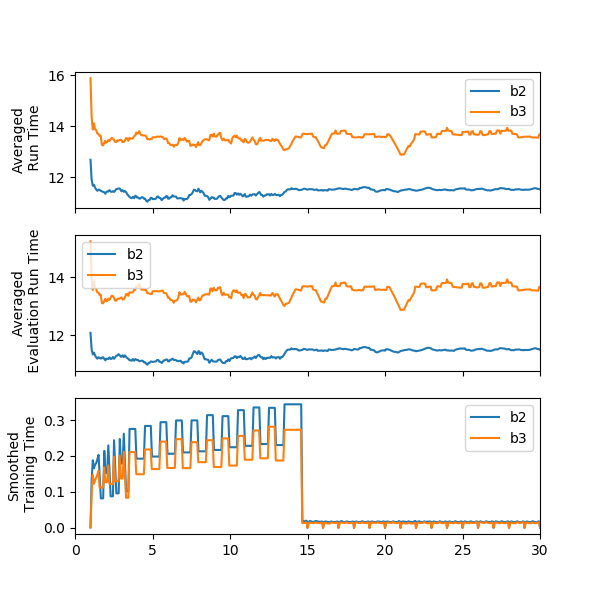
\includegraphics{b2_b3_time.png} &
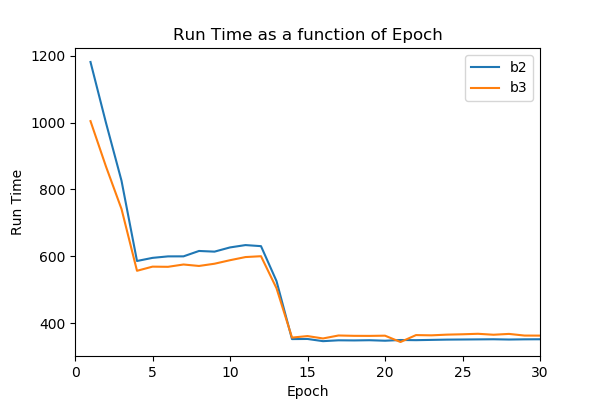
\includegraphics{b2_b3_epoch.png} & 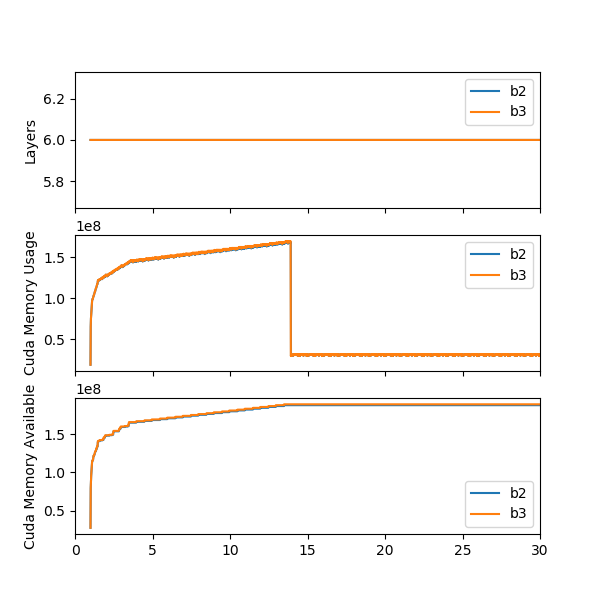
\includegraphics{b2_b3_memory.png} &
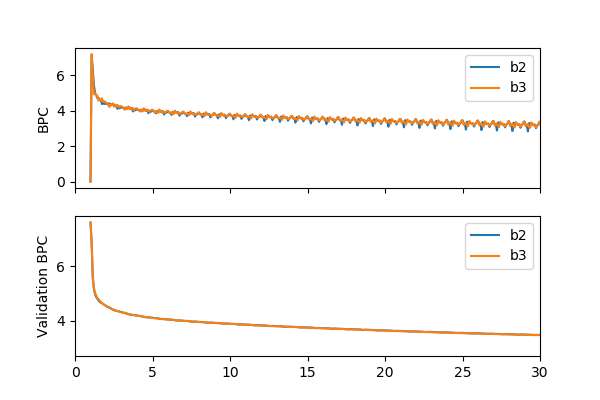
\includegraphics{b2_b3_frac.png} &
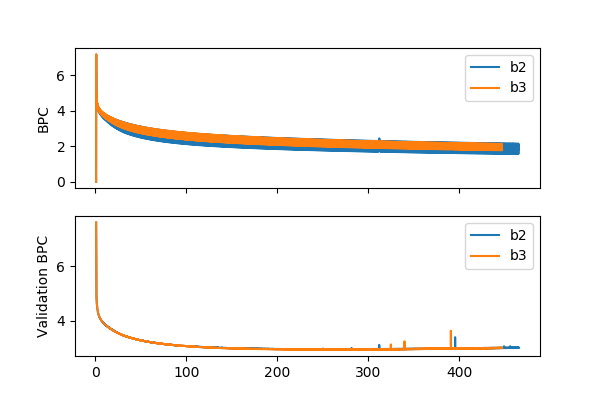
\includegraphics{b2_b3_frac_full.png}\tabularnewline
l & 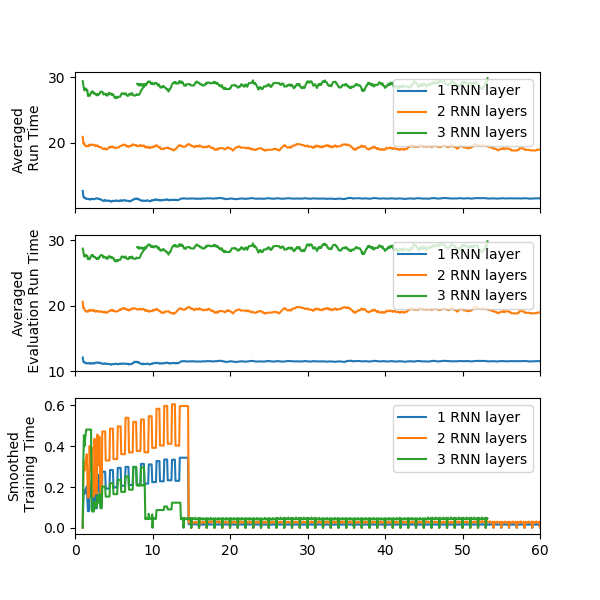
\includegraphics{l_time.png} & 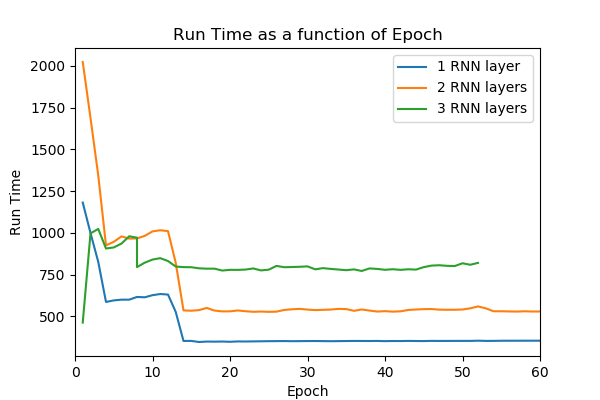
\includegraphics{l_epoch.png} &
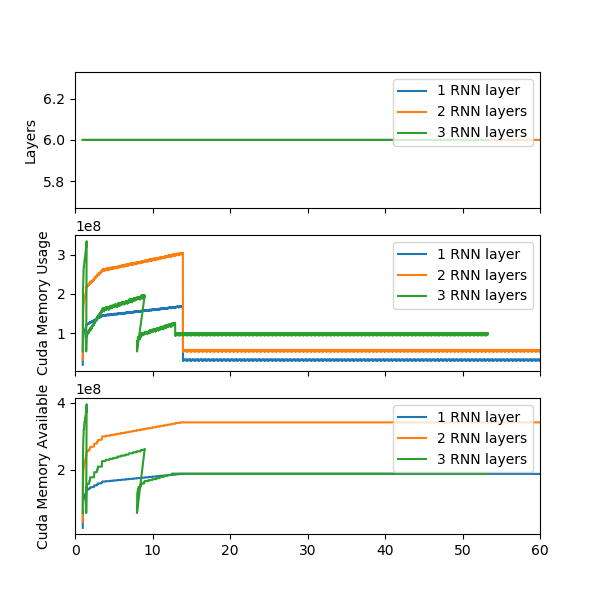
\includegraphics{l_memory.png} & 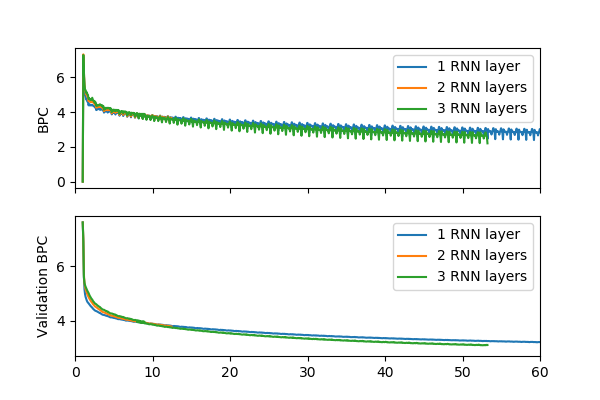
\includegraphics{l_frac.png} &
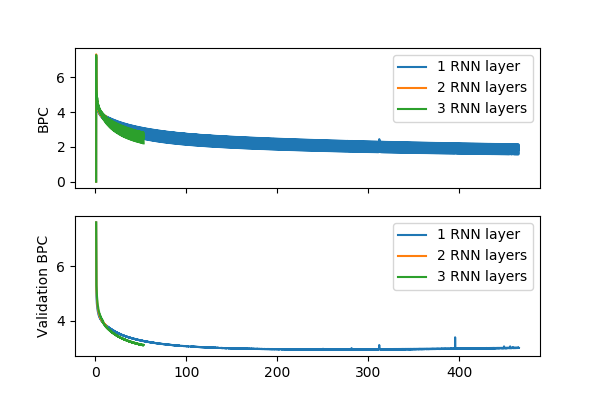
\includegraphics{l_frac_full.png}\tabularnewline
lbl & 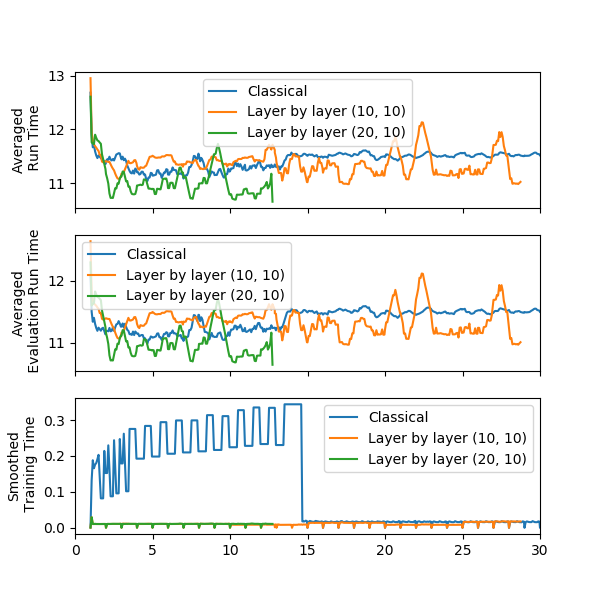
\includegraphics{lbl_time.png} & 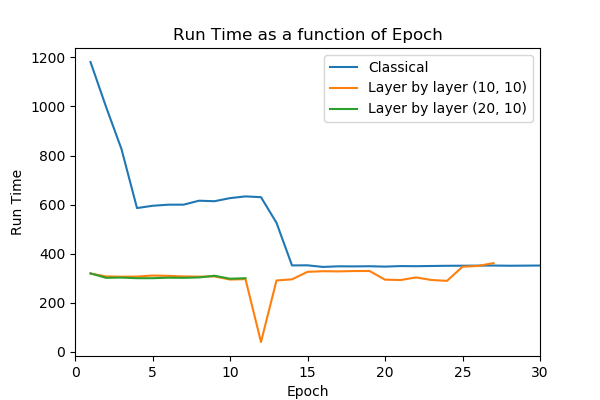
\includegraphics{lbl_epoch.png} &
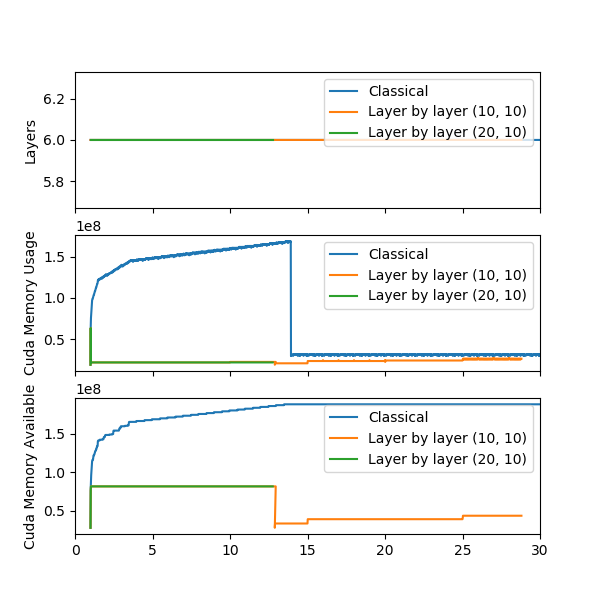
\includegraphics{lbl_memory.png} & \includegraphics{lbl_frac.png} &
\includegraphics{lbl_frac_full.png}\tabularnewline
sum & \includegraphics{sum_time.png} & \includegraphics{sum_epoch.png} &
\includegraphics{sum_memory.png} & \includegraphics{sum_frac.png} &
\includegraphics{sum_frac_full.png}\tabularnewline
\bottomrule
\end{longtable}

Plots will be referred to with : (Ex: ``l:Memory'')

\subsubsection{Time necessary to reach indicated validation
BPC}\label{time-necessary-to-reach-indicated-validation-bpc}

\begin{longtable}[]{@{}lrrr@{}}
\toprule
Model & 5 BPC & 4 BPC & 3 BPC\tabularnewline
\midrule
\endhead
b2 & 0H 19M 41S & 1H 19M 47S & 15H 13M 7S\tabularnewline
b3 & 0H 16M 44S & 1H 11M 48S & 15H 3M 22S\tabularnewline
s & 0H 5M 19S & 0H 30M 59S &\tabularnewline
s-a20-l10 & 0H 5M 19S & 0H 30M 26S &\tabularnewline
l2 & 0H 33M 43S & 2H 27M 51S &\tabularnewline
l3 & \sout{0H 7M 41S} & \sout{2H 13M 2S} &\tabularnewline
s\_l3\_a & 0H 16M 7S & &\tabularnewline
\bottomrule
\end{longtable}

Empty fields are where network has not reached BPC yet \sout{Crossed
out} fields are where data has been corrupted (because of an
interruption in training)

\subsubsection{Epochs necessary to reach indicated validation
BPC}\label{epochs-necessary-to-reach-indicated-validation-bpc}

\begin{longtable}[]{@{}llll@{}}
\toprule
Model & 5 BPC & 4 BPC & 3 BPC\tabularnewline
\midrule
\endhead
b2 & 0.296 & 6.000 & 141.4\tabularnewline
b3 & 0.367 & 5.954 & 136.4\tabularnewline
s & 0.371 & 6.000 &\tabularnewline
s-a20-l10 & 0.371 & 6.000 &\tabularnewline
l2 & 0.593 & 6.519 &\tabularnewline
l3 & 0.816 & 7.296 &\tabularnewline
s\_l3\_a & 1.148 & &\tabularnewline
\bottomrule
\end{longtable}

Empty fields are where network has not reached BPC yet

\subsection{Analysis}\label{analysis}

\subsubsection{\texorpdfstring{Run time and memory on ``l'' series
(l:memory, l:time, and l:time to run an
epoch)}{Run time and memory on l series (l:memory, l:time, and l:time to run an epoch)}}\label{run-time-and-memory-on-l-series-lmemory-ltime-and-ltime-to-run-an-epoch}

Training of ``l3'' model was interrupted 2 times before the 15th epoch,
each time cleaning the memory, inducing training time reduction and
epoch time reduction (due to the correlation of memory usage and
training time).

\subsubsection{\texorpdfstring{Run time and memory on ``lbl'' series
(lbl:memory, lbl:time, and lbl:time to run an
epoch)}{Run time and memory on lbl series (lbl:memory, lbl:time, and lbl:time to run an epoch)}}\label{run-time-and-memory-on-lbl-series-lblmemory-lbltime-and-lbltime-to-run-an-epoch}

The specificity of layer by layer training are a lead to the cause of
the collapse of memory usage and run time during the 15th epoch.

During layer by layer training, memory usage is kept constant over the
first 15 epochs, whereas with classical training, memory usage increases
during ths period.

Layer by layer training reduces simultaneous graph accumulation over the
different epochs by training a layer at a time. It possibly reduces SGD
inertia too.

\subsubsection{Performance of layer by layer
training}\label{performance-of-layer-by-layer-training}

No notable variation on BPC. For run time and memory, see above.

\subsubsection{Performance of multi-RNN-layered
architecture}\label{performance-of-multi-rnn-layered-architecture}

A slight improvement of BPC can be seen with 3 layers (sadly, BPC data
for 2 layers is corrupted). Computation-time is proportional to the
number of layers (time data for 3 layers is unusable).

\subsubsection{Performance of 3 batches compared to 2
batches}\label{performance-of-3-batches-compared-to-2-batches}

2 and 3 batches have an almost identical performance (time-wise,
BPC-wise and memory-wise), except 3 batches seem to get less dispersed
BPC.

\subsubsection{Results of long training with 2 and 3 batches
(b2\_b3:full length
bpc)}\label{results-of-long-training-with-2-and-3-batches-b2_b3full-length-bpc}

The plot ``b2\_b3:full length bpc'' shows that after 200 epochs,
validation BPC stagnates. After 300 epochs, validation BPC begins to
increase very slowly, those are the first signs of over-fitting. These
observations were cross-checked with the raw data.

\subsubsection{Note on attention module}\label{note-on-attention-module}

A model with the attention module was tested for 5 hours, and did not
reach a full epoch. It can be deemed that without a training algorithm
like layer by layer training, using attention is not viable.

\end{report}





%\input{parts/appendix/reports-gmsnn/docs_esteban-latex/}
\cleardoublepage

\chapter{Rapports d'avancement du \glsentrytext{project_papud}}
\section{Informations sur les documents contenus dans la présente annexe}
Les sections suivantes contiennent les rapports intermédiaires fournis à notre maître de stage et au autres membres du projet au cours du \gls{project_papud}.

\subsection{Format d'origine, transcription et contenu des rapports}
Pour les mêmes raisons que pour l'annexe précédente (décrite dans la \autoref{report_infos}), les documents présentés dans cette annexe ont été rédigés en anglais, au format \gls{git_md}; les versions présentées ici sont des transcriptions aussi fidèles que possible de ces documents.

\newpage
\begin{report}{Informations générales}
	\section*{General information}

\subsection{Corpus}

\subsubsection{firsttest}

\paragraph{Baseline accuracy}

True baseline accuracy (for char \lstinline!-!): training 0.443; valid
0.414; test 0.423

\begin{longtable}[]{@{}llll@{}}
\hline
char & training & valid & test\tabularnewline
\hline
\endhead
\lstinline!-! & \textbf{0.443} & \textbf{0.414} & \textbf{0.423}\tabularnewline
\lstinline! ! & 0.064&0.067&0.063\tabularnewline
\lstinline!a! & 0.021&0.022&0.023\tabularnewline
\lstinline!0! & 0.015&0.013&0.011\tabularnewline
\lstinline!<unk>! & 0.0&0.0&0.0\tabularnewline
\hline
\end{longtable}

\subsection{Grid-5000}

To develop and train the model, we are using Grid-5000 computers
clusters. For specific information on Grid-5000, see
\href{https://www.grid5000.fr/}{https://www.grid5000.fr/}.

\subsubsection{GPU-equipped nodes}

Due to the properties of neural networks models, it is really efficient
to use GPUs to train them.

Here are the main GPU-equipped nodes of Grid-5000:

\begin{longtable}[]{@{}rcrrcc@{}}
\hline
Nodes & GPU & Graphical memory & RAM & Production & CUDA\tabularnewline
\hline
\endhead
graphique-1 & 2 x Nvidia Titan Black & 2 x 6GB & 64GB & X &
2880\tabularnewline
graphique-2/6 & 2 x Nvidia GTX 980 & 2 x 4GB & 64GB & X &
2048\tabularnewline
graphite-1/4 & Intel Xeon Phi 7120P & 16GB & 256GB & & ?\tabularnewline
grele-1/14 & 2 x Nvidia GTX 1080 Ti & 2 x 11GB & 128GB & X &
3584\tabularnewline
grimani-1/6 & 2 x Nvidia Tesla K40M & 2 x 12GB & 64GB & X &
2880\tabularnewline
\hline
\end{longtable}

\section*{{[}NOT TESTED YET{]} Model conversion}

See 
\href{https://github.com/ysh329/deep-learning-model-convertor}{https://github.com/ysh329/deep-learning-model-convertor}

\end{report}
\begin{report}{Résultats de l'implémentation basique}
	\section*{Results of the basic implementation of the
model}

2018/07/09 - SYNALP - Esteban MARQUER

\subsection{Paradigm}

The test is run on a minimal number of epoch (10), with a minimal model.

The training algorithm used is an example by example training.

\subsubsection{Model architecture}

The model is a line by line predictive model, composed of: - a character
embedding layer; - a pooling layer; - a linear layer; - an output layer.

The output of the model is a probability distribution over known
characters for every character of the predicted line.

\subsection{Results}

\subsubsection{GPU memory usage}

As expected from the model architecture, GPU memory usage is constant.

\begin{figure}[ht]
\centering
\includegraphics{parts/appendix/reports-papud/2018_07_09-Basic_implementation_results/memory.png}
\caption{memory usage}
\end{figure}

\subsubsection{Computation time}

\subsubsection{Loss and accuracy}

The loss used is cross-entropy loss, a character per character
negative-log-likelihood loss over the soft-maxed distribution.

Overall, the loss gives a score to the prediction of the model, by
comparing the target character and a distribution of probabilities for
each character. If the probability for the target character is high and
other character low, the model does a good prediction of the character,
and the score given is low. The closer the score is to 0, the better it
is. The scores of each characters is averaged, producing a global loss
over the line.

Accuracy is a percentage. The closer to 100 \% the better. As the loss
is bound by 0 and +Infinity, and the closer to 0 the better, a correct
transformation to accuracy could be: \lstinline!exp(-loss)! for an
accuracy between 0 and 1.

\begin{figure}[ht]
\centering
\includegraphics{parts/appendix/reports-papud/2018_07_09-Basic_implementation_results/loss.png}
\caption{loss}
\end{figure}

The small spike recurrently appearing in the loss and accuracy is most
likely due to a noisy part of the corpus (around the middle of the
corpus) causing the model to learn wrongly on those specific examples.

The best precision obtained at the end of 10 epochs is 50\%,
corresponding to a loss of about 0.7.

\subsection{Improvements and next
steps}

\subsubsection{Mini-batch}

Currently, the models learn one example at a time, meaning it computes
the result for a line of input, compares it to the target, and updates
weights. A common algorithm is the mini-batch algorithm, computing
simultaneously a set of examples, their loss compared to the target, and
updates the weights of the model all at once for the whole set of
examples.

This algorithm speeds-up training while making the most of the GPU.

\subsubsection{Dynamic corpus}

While with the current corpus there is no real problem in storing the
whole corpus in the memory, the future corpus will be over 400GB of
text. It is necessary to replace the current method by a dynamic loading
and transformation of the parts of the corpus currently used by the
model. An ideal solution would be to read the target data directly from
the archive containing the corpus.

\end{report}
\begin{report}{Paquets (\foreign{batchs}) simultanés}
\section*{Increasing the number of simultaneous
examples}

2018/07/10 - SYNALP - Esteban MARQUER

\subsection{Paradigm}

The test is run on a small number of epoch (20), with a minimal model
and a new training algorithm.

The training algorithm used is a \textbf{mini-batch training}, meaning
we compute the output for multiple examples all at once, we compute an
averaged loss over those examples, and we update the model.

The potential effects of this algorithm are:
\begin{itemize}
\item an increase of GPU memory usage, as computations are done on larger data;
\item a decrease of computation time, with the number of computations reduced;
\item a smother training loss, because it is averaged over multiple examples;
\item avoidance of some local minima.
\end{itemize}

A second test with random batch-size between 1 and 1000 was done on 50
epoch, to evaluate the effect of the batch size and find an optimum.

\subsection{Results}

\subsubsection{GPU memory usage}

As more examples are fed to the model, there is a very slight increase
in GPU memory usage: 0.013e7 B, corresponding to 127kiB (this amount is
negligible with more than 10GiB available and a current usage of about
10MiB).

\textbf{Conclusion:} increasing the number of simultaneous examples has
no substantial downsides memory-wise.

\begin{figure}[ht]
\centering
\includegraphics{parts/appendix/reports-papud/2018_07_11-Simultaneous_batches/memory.png}
\caption{memory usage}
\end{figure}

\subsubsection{Loss and accuracy}

As loss is averaged on multiple examples, it should be smoother. But,
probably because the number of simultaneous examples is too small, there
is no noticeable change of loss, with the curves superposed.

\textbf{Conclusion:} increasing the number of simultaneous examples has
no substantial effect loss-wise.

\begin{longtable}[]{@{}lll@{}}
\hline
Train. + Valid. & Training only & Validation only\tabularnewline
\hline
\endhead
\includegraphics[width=.3\textwidth]{parts/appendix/reports-papud/2018_07_11-Simultaneous_batches/loss.png} & \includegraphics[width=.3\textwidth]{parts/appendix/reports-papud/2018_07_11-Simultaneous_batches/loss_train.png} &
\includegraphics[width=.3\textwidth]{parts/appendix/reports-papud/2018_07_11-Simultaneous_batches/loss_valid.png}\tabularnewline
\hline
\end{longtable}

\subsubsection{Computation time}

The computations done on GPU benefit from grouping similar operations.
By computing multiple examples together, we can use this property to
speed up training. Moreover, retro-propagation and model updates are
less frequent, reducing computational load and training time.

The best-case time allow an improvement from 10ms to less than 2ms per
\textbf{training} sequence with a batch-size of 50, and the worst-case
one allow 4ms per training sequence with a batch-size of 200.

A small gain can be achieved on \textbf{validation} time by increasing
batch size over 50, but increasing it more has no effect.

\textbf{Conclusion:} increasing the number of simultaneous examples
leads to a notable improvement of computation time.

\begin{longtable}[]{@{}ll@{}}
\hline
Training time & Validation time\tabularnewline
\hline
\endhead
\includegraphics[width=.45\textwidth]{parts/appendix/reports-papud/2018_07_11-Simultaneous_batches/sequence_time.png} &
\includegraphics[width=.45\textwidth]{parts/appendix/reports-papud/2018_07_11-Simultaneous_batches/valid_time.png}\tabularnewline
\includegraphics[width=.45\textwidth]{parts/appendix/reports-papud/2018_07_11-Simultaneous_batches/sequence_time_.png} &
\includegraphics[width=.45\textwidth]{parts/appendix/reports-papud/2018_07_11-Simultaneous_batches/valid_time_.png}\tabularnewline
\hline
\end{longtable}

\subsection{Conclusion}

Even if there is no improvement of loss or memory, the gain in
computation time is enough to accept this algorithm.

The ideal batch-size (with the current node ``grele'') is between 50 and
200. In future works, a batch-size of 200 will be used, as it present
the best worst- and best-case time performances.

\subsection{Improvements and next
steps}

\subsubsection{Dynamic corpus}

The dynamic corpus implementation is ready (except small details) and
working, only integration is left.

\paragraph{Buffer size}

The dynamic corpus can use a buffer, and the size of this buffer must be
at least the size of the batch. It will be necessary to test which size
is optimal. An optimal buffer has the minimal size to make computation
time over the buffer size only slightly higher than pre-loading time. It
allows training to continue without interruption, while maintaining a
low memory usage.

\end{report}
\begin{report}{Analyse du pic de performance}
\section*{Performance spike analysis}

2018/07/18 - SYNALP - Esteban MARQUER

\subsection{Problem}

During training, a big performance spike appeared periodically. It is
necessary to know why this spike appeared.

The different parts of the spike are:
\begin{itemize}
\item from line 24545 to line 31558 (35\% to 45\% of the corpus): the increase of the BPC;
\item from line 31558 to line 36468 (45\% to 52\% of the corpus): a stable part at a high value;
\item from line 36468 to line 38572 (52\% to 55\% of the corpus): the decrease of the BPC.
\end{itemize}

\begin{longtable}[]{@{}ll@{}}
\hline
Loss of 1 epoch (first epoch) & Zoom on spike\tabularnewline
\hline
\endhead
\includegraphics[width=.45\textwidth]{parts/appendix/reports-papud/2018_07_18-Performance_spike_analysis/loss_valid.png} &
\includegraphics[width=.45\textwidth]{parts/appendix/reports-papud/2018_07_18-Performance_spike_analysis/loss_valid_part.png}\tabularnewline
\hline
\end{longtable}

\subsection{Analysis}

By extracting the parts of the corpus corresponding to the parts of the
spike, and scrolling through them, some recurrent elements appear: -
lines beginning by \lstinline!kern!, more specifically
\lstinline!kern info! and \lstinline!kern debug!; - lines containing a
memory address, like \lstinline!0x91ffffff!, \lstinline!0x0093! and
\lstinline!00000000fed18000!, or an error code like \lstinline!0x0100!,
- lines beginning by \lstinline!daemon!, more specifically
\lstinline!daemon err!;

The most interesting part of the spike is the increase of the BPC, were
the performance deteriorate.

Given the repartition and percentages (see the next two sub-sections),
the most likely causes for the spikes are:
\begin{itemize}
\item the memory address and
hexadecimal codes;
\item the kernel messages (very repetitive, and
containing memory address and hexadecimal codes).
\end{itemize}

\paragraph{Examples of Kernel
messages}

\begin{lstlisting}
kern info kernel ACPI: LAPIC (acpi_id[0x00] lapic_id[0x00] enabled)
kern info kernel ACPI: LAPIC (acpi_id[0x02] lapic_id[0x02] enabled)
kern info kernel ACPI: LAPIC (acpi_id[0x04] lapic_id[0x04] enabled)
kern info kernel ACPI: LAPIC (acpi_id[0x06] lapic_id[0x06] enabled)
kern info kernel ACPI: LAPIC (acpi_id[0x08] lapic_id[0x08] enabled)
\end{lstlisting}

\subsubsection{Repartition of match in the
corpus}

The ``localisation bars'' (vertical blue lines) delimit to the different
parts of the spike.

\begin{longtable}[]{@{}lll@{}}
\hline
Type of element & With localisation bars & With
subcategories\tabularnewline
\hline
\endhead
Memory addresses & \includegraphics[width=.25\textwidth]{parts/appendix/reports-papud/2018_07_18-Performance_spike_analysis/memory_.png} &
\includegraphics[width=.25\textwidth]{parts/appendix/reports-papud/2018_07_18-Performance_spike_analysis/memory.png}\tabularnewline
Kernel process & \includegraphics[width=.25\textwidth]{parts/appendix/reports-papud/2018_07_18-Performance_spike_analysis/kern_.png} &
\includegraphics[width=.25\textwidth]{parts/appendix/reports-papud/2018_07_18-Performance_spike_analysis/kern.png}\tabularnewline
Daemon process & \includegraphics[width=.25\textwidth]{parts/appendix/reports-papud/2018_07_18-Performance_spike_analysis/daemon_.png} &
\includegraphics[width=.25\textwidth]{parts/appendix/reports-papud/2018_07_18-Performance_spike_analysis/daemon.png}\tabularnewline
All types & & \includegraphics[width=.25\textwidth]{parts/appendix/reports-papud/2018_07_18-Performance_spike_analysis/all.png}\tabularnewline
\hline
\end{longtable}

\subsubsection{Percentages of match in each part of the
corpus}

Percentages of match are percentages on the total line number of the
part of the corpus analysed.

\begin{lstlisting}
--- spike up slope (lines 24545 to 31558, 35% to 45%) ---
Total lines:  7013
Matching "kern .*": 2888 (41%)
Matching "kern info .*": 1458 (20%)
Matching "kern debug .*": 1172 (16%)
Matching "daemon .*": 2048 (29%)
Matching "daemon err .*": 935 (13%)
Matching any memory pattern: 1728 (24%)
Matching "0x[0-9,a-f]{8}": : 196 (2%)
Matching "[0-9,a-f]{16}": : 250 (3%)
Matching "0x[0-9,a-f]*?": : 1478 (21%)

--- spike flat (lines 31558 to 36468, 45% to 52%) ---
Total lines:  4910
Matching "kern .*": 4218 (85%)
Matching "kern info .*": 2154 (43%)
Matching "kern debug .*": 1760 (35%)
Matching "daemon .*": 346 (7%)
Matching "daemon err .*": 174 (3%)
Matching any memory pattern: 1149 (23%)
Matching "0x[0-9,a-f]{8}": : 294 (5%)
Matching "[0-9,a-f]{16}": : 296 (6%)
Matching "0x[0-9,a-f]*?": : 853 (17%)

--- spike down slope (lines 36468 to 38572, 52% to 55%) ---
Total lines:  2104
Matching "kern .*": 27 (1%)
Matching "kern info .*": 15 (0%)
Matching "kern debug .*": 0 (0%)
Matching "daemon .*": 383 (18%)
Matching "daemon err .*": 15 (0%)
Matching any memory pattern: 90 (4%)
Matching "0x[0-9,a-f]{8}": : 34 (1%)
Matching "[0-9,a-f]{16}": : 5 (0%)
Matching "0x[0-9,a-f]*?": : 85 (4%)

--- whole spike (lines 24545 to 38572, 35% to 55%) ---
Total lines:  14027
Matching "kern .*": 7133 (50%)
Matching "kern info .*": 3627 (25%)
Matching "kern debug .*": 2932 (20%)
Matching "daemon .*": 2777 (19%)
Matching "daemon err .*": 1124 (8%)
Matching any memory pattern: 2967 (21%)
Matching "0x[0-9,a-f]{8}": : 524 (3%)
Matching "[0-9,a-f]{16}": : 551 (3%)
Matching "0x[0-9,a-f]*?": : 2416 (17%)

--- full corpus ---
Total lines:  70131
Matching "kern .*": 10972 (15%)
Matching "kern info .*": 5298 (7%)
Matching "kern debug .*": 4134 (5%)
Matching "daemon .*": 10828 (15%)
Matching "daemon err .*": 1504 (2%)
Matching any memory pattern: 5859 (8%)
Matching "0x[0-9,a-f]{8}": : 1586 (2%)
Matching "[0-9,a-f]{16}": : 893 (1%)
Matching "0x[0-9,a-f]*?": : 4987 (7%)

Matching "kern .*" outside of spike: 3839 (5%)
\end{lstlisting}

\subsection{Conclusion(s)}

There are two possible conclusions:
\begin{itemize}
\item the kernel messages are the cause of the spike;
\item or the memory addresses and hexadecimal codes are the cause of the spike.
\end{itemize}

\subsubsection{Kernel messages}

If the kernel messages are the cause of the spike, the most likely
explanation is that this part of the corpus represent a crash of the
server or a major error. In that case, we must remove that part of the
corpus from the training set, as it is not the ``normal'' evolution of
the log.

\subsubsection{Memory addresses and hexadecimal codes}

If the memory addresses and hexadecimal codes are the cause of the
spike, it should be because a succession of number is a very specific
thing to learn. In that case, either we let the model learn the brute
codes, or we replace every code by a ``<hex>'' character to ease the learning
process. It is also possible to replace the different kind of code by a
different character.

\subsection{Improvements and next steps}

To check whether the memory addresses and hexadecimal codes, or the
kernel messages are the cause of the spike, trying to train the model
while replacing every code by a ``<hex>'' character. If there is no
improvement, then the codes are not the cause of the performance spike.

\end{report}
\begin{report}{Rapport de la réunion avec les autres membres du projet}
\section*{Team meeting report}

2018/07/20 - SYNALP - Esteban MARQUER

\subsection{Main points}

\begin{itemize}
\item
  Performance spike issue: see report
  ``2018\_07\_18-Performance\_spike\_analysis''

  \begin{itemize}
  \item
    solution chosen: replace hexadecimal codes with a special label per
    kind of code
  \end{itemize}
\item
  Long training: no over-fitting, 90\% accuracy in 500 epochs

  \begin{longtable}[]{@{}ll@{}}
  \hline
  sequence by sequence mesure & epoch summary\tabularnewline
  \hline
  \endhead
  \includegraphics[width=.45\textwidth]{parts/appendix/reports-papud/2018_07_20-500_epochs/accuracy.png} &
  \includegraphics[width=.45\textwidth]{parts/appendix/reports-papud/2018_07_20-500_epochs/accuracy_epoch.png}\tabularnewline
  \includegraphics[width=.45\textwidth]{parts/appendix/reports-papud/2018_07_20-500_epochs/loss.png} &
  \includegraphics[width=.45\textwidth]{parts/appendix/reports-papud/2018_07_20-500_epochs/loss_epoch.png}\tabularnewline
  \hline
  \end{longtable}
\item
  Baseline accuracy: see first section of ``General\_information.md''
  for values.

  \begin{itemize}
  \item
    Baseline accuracy is high with padding (about 50\%), perhaps lines
    are too long (a lot of padding is needed)
  \item
    Compared with performance, performance is still good
  \end{itemize}
\item
  GPU usage with compleetely loaded corpus: 30\% to 60\%

  \begin{itemize}
  \item
    This is bad new, with such a model training should go at 99\% al the
    time
  \item
    It is necessary to locate the element slowing the process, try
    removing all unecessary processes (logging, storage in memory,
    accuracy, \ldots{})
  \end{itemize}
\item
  New corpus implementation (with buffer and iterators): about
  180s/epoch, 65s/epoch with old implementation (everything loaded in
  memory)

  \begin{itemize}
  \item
    a good implementation of the data loading is critical
  \item
    perhaps pre-loading is too slow because of computations, a
    pre-processed version could help
  \item
    training the model multiple time on a loaded segment could bridge
    the gap between the two processes used
  \item
    using more processes could do the trick (one for loading only, one
    for processing, and one for training)
  \item
    using ``binary''-sized batches (like 8, 64 or 1024) is said to
    achieve faster results, maybe a bit of speed can be gained there
  \end{itemize}
\item
  Development of a learning rate optimisation script: good, better if
  offline (good if both online and offline)

  \begin{itemize}
  \item
    online stands for optimisation before, or/and during every training
  \item
    offline stands for an analysis done a single time, aside from any
    training
  \end{itemize}
\end{itemize}

\subsection{Improvements and next
steps}

\begin{itemize}
\item
  Finish the development of learning rate optimisation.
\item
  Try to make the corpus implementation clean and fast enough (with
  compared run times).
\item
  Integrate the modifications of the corpus processing (memory address
  management)
\item
  Use ``binary''-sized batches; 128 seems perfect, as it is between 50
  and 200 (the bounds found when optimising batches).
\end{itemize}

\end{report}
\begin{report}{Optimisation du taux d'apprentissage}
\section*{Learning rate optimisation}

2018/07/23 - SYNALP - Esteban MARQUER

\subsection{General information}

Learning rate is an hyperparameter in the training algorithm which
changes the speed of the training and the performance of the model.
Specifically, it is a coefficient of the gradient used to update the
parameters of the model.

There are three main learning rates for a model:
\begin{itemize}
\item a learning rate that is too small (closer to 0): the training is slow, and can get blocked in some local minima;
\item a learning rate that is too high (closer to +infinity, usually closer to 1): the learning is faster and avoid local minima, but could diverge from the solution;
\item a balanced learning rate: what we want to find, the traing is fast yet does not diverge.
\end{itemize}

\subsection{Optimisation process}

Usually, learning rate optimisation is done with a logarithmic scale of
the learning rate. The shape of the produced curves confirm the use of
such a scale.

The optimisation process is driven by three parameters and a single
metric.

The metric is the accuracy of the model on the validation corpus at the
end of the training.

The parameters are: the two bounds of the learning rate, and the
learning rate variation factor: the ``learning rate multiplier''.

The learning rate varies as follow in the psedo-python algorythm:

\begin{lstlisting}[language=Python]
# the learning rate takes the highest value as start value, as it will decrease over time
learning_rate = start_value 

# until the learning rate as reach the stop value (the lowest of the two bounds), we make it vary logarithmically
while learning_rate > stop_value:
    performance = train_model(learning_rate)
    save_model_performance(performance, learning_rate)
    
    # the learning rate is updated
    # example with a learning rate of 1 and a learning rate multiplier of 0.1:
    # at first the learning rate is 1, then 0.1, then 0.01 ...
    learning_rate = learning_rate * learning_rate_multiplier

# we compare the performance of the model with the different learning rates
compare_model_performance()
\end{lstlisting}

The closer to 0 the learning rate multiplier is, the faster the
variation will be, and the closer to 1 it si, the slower the variation
will be. To have a decent resolution in the curves, a multiplier close
to 1 is crucial.

The training is done each time on a full epoch.

\subsection{Results}

The first plot is done with a learning rate between 1 and 10\^{}(-5),
with a multiplier of 0.2. The second one is done with a learning rate
between 1 and 10\^{}(-2), with a multiplier of 0.6 (the total of dots is
10).

\includegraphics{parts/appendix/reports-papud/2018_07_23-Learning_rate_optimisation/lr_epoch_1_mul_0_2.png}
\includegraphics{parts/appendix/reports-papud/2018_07_23-Learning_rate_optimisation/lr_epoch_1_mul_0_6_best_0_216.png}

There is a strange accuracy at the end of the first plot: the
theoretically unreachable 0\%. It is confirmed by the second plot, with
multiple points having an accuracy of 0\%. With a baseline accuracy of
44\%, it is clear that the result diverge from wat is expected. It is a
case of divergence due to a learning rate that is too high.

The best learning rate found is 0.216 (0.6\^{}3), giving the fastest
learning (over 90\% of accuracy in 1 epoch) without diverging.

\subsection{Additional information}

The current implementation consist of a script building a model, and
finding the ideal learning rate for this model. It is an offline
implementation of the model.

The way it is implemented is ideal for an online use too, as the only
operation needed are the removal of the plotting part, and adding the
reload of the model with an updated learning rate.

\subsection{Improvements and next
steps}

Use the new learning rate in the training. As it is quite close to
diverge, it would be advised to use a slightly lower learning rate like
0.2.

If inline optimisation is used, three possibilities seem viable: -
choosing the learning rate every time we start a training, to adapt to
the current hyperparameters; - updating the learning rate every set
number of epochs, to adapt the learning to the current state of the
model; - doing each epoch with a set of learning rates, and every time
choosing the best result; even if costly (every epoch is done multiple
time), it should allow a really fast learning with lowered chances of
divergence or over-fitting.

Personally, my preferred option is the second one.

\end{report}
\begin{report}{Effets de l'optimisation du taux d'apprentissage}
\section*{Learning rate optimisation effect on learning
curve}

2018/07/24 - SYNALP - Esteban MARQUER

\subsection{Context}

The previous results of learning rate optimisation lead to a potentially
optimal learning rate of 0.2 (instead of 0.001).

A run with the new learning rate and every other thing identical was
done to compare performance to previous 500 epoch run. That specific run
had a learning rate of 0.001.

\subsection{Results}

The new learning rate has two effects: 1. convergence is achieved in
less than 100 epoch, compared to previous learning achieving convergence
in more than 400 epochs; 2. a small but constant gap between training
performance and validation performance, but it is not over-fitting (if
both training and validation are constant, we can not conclude that the
model over-fits).

\begin{figure}[ht]
\centering
\includegraphics{parts/appendix/reports-papud/2018_07_24-Learning_rate_optimisation_effect/accuracy.png}
\caption{accuracy}
\end{figure}

\subsection{Conclusion}

The new learning rate is better than the previous one, it will be kept.

\subsection{Improvements and next
steps}

{[}OPTIONAL{]} Use inline optimisation to update the learning rate every
set number of epochs (once convergence is reached).

\end{report}
\begin{report}{Taille de \foreign{batch} binaire}
\section*{Binary batch size effect on run
speed}

2018/07/26 - SYNALP - Esteban MARQUER

\subsection{Context}

It has been said that batches using binary sizes (64, 256, 1024,
\ldots{}) perform faster than non-binary sises.

\subsection{Paradigm}

To verify this phenomenon and perhaps improve the training speed, a
comparative experiment has been done with a batch size of 128 and a
batch size of 200.

\subsection{Results}

There is notable no effect, except the effect predicted by the batch
size comparision done previously, and stating that batches with a size
of 200 are faster than with a size of 128.

\begin{figure}[ht]
\centering
\includegraphics{parts/appendix/reports-papud/2018_07_26-Binary_batch_size/time_epoch.png}
\caption{time per epoch}
\end{figure}

\subsection{Conclusion}

The most straightforward conclusion is that either the effect of binary
sizes is negligible if not non-existent, or there is a hidden parameter
changing th true size of the data (for example a set of bytes used to
store metadata together with the regular data).

As the previous batch size (200) performs better, we will keep it.

\subsection{Next steps and
improvements}

Investigating a potentially non-existent effect (at least with the
current model) does not seem efficient considering the potential gain in
computation time (compared to improving the naive model).

No further work will be done on that now (at least for now).

\end{report}
\begin{report}{Performances du lecteru de corpus multi-fichiers multi-processus}
\section*{Learning rate optimisation effect
on}

2018/07/26 - SYNALP - Esteban MARQUER

\subsection{Context}

Given the large amount of data to process, and the way it is structured
in many small archives, a way to load and pre-process them efficiently
had to be implemented.

\subsection{Multi-file-multi-process corpus
concept}

\subsubsection{Multi-process system}

To avoid the need to completely pre-processing the data and storing it,
and to shift the computational weight of the loading process, the
different tasks are splitted between multipple processes.

At first, the idea was to use three processes, with one for the loading,
one for the pre-processing, and the lat one for the transformation into
tensor. All those process fetch data from a multiprocess-safe queue and
store the result in an output queue, used by the next process as an
input.

A representation of the initial concept:

\begin{lstlisting}
HDD -> Loader -> [raw data queue]
    -> Processing -> [processed data queue]
    -> Tensorising -> [tensors queue]
    -> model
\end{lstlisting}

Given the performance of that system, the slowest part was the
processing. Moreover, the processing could be splitted in multiple
modules: removing the end-of-line characters, replacing paterns by tags
and splitting into characters, transforming the data via a dictionary,
and padding/cropping the sequence.

A representation of the modular processing concept:

\begin{lstlisting}
HDD -> Loader -> [raw Q.]
    -> Process 1 -> [partially processed Q. 1]
    -> Process 2 -> [partially processed Q. 2]
    ...
    -> Process n -> [processed Q. n]
    -> Tensorising -> [tensors queue]
    -> model
\end{lstlisting}

This architecture allows to change the order of the pre-processing
modules, and to add or remove some of them.

By splitting those different tasks on multipple processes, an efficient
processing is achieved. Moreover, it is way easier to add pre-processing
steps.

\subsubsection{Multi-file system}

By considering a set of files as a single sequence of line, and by
loading only the one file containing the current data, combined by
efficient line-by-line sequential reading, a light and fast loading is
achieved.

\subsection{Tests}

\subsubsection{Paradigm}

While setting up the unitary tests for the corpus implementations, three
main situations have produced useful insight on the performances of the
new implementations.

Everything was run on my laptop, with other processes running that may
have hindered the performance (for example, a heavy IDE).

Process-specific tests were run after every element was proven to do
their expected job. Those tests added the processes and the data queues
and information on queue filling and process state.

\subsubsection{Results}

Multiple test were done with very light, light treatment of the data,
and real-situation training (the training is a way to process the data).

\paragraph{Printing only the status of the process at each
batch}

Total time per epoch 12 s

\begin{lstlisting}[language=Python]
{'example': '28032/67923',
 'batch': '218/527',
 'iterator status':
   'Process MultiFile status: process: alive; output queue: 1023/1024
    Process EndLine status: process: alive; output queue: 1023/1024
    Process Regex status: process: alive; output queue: 1024/1024
    Process Dictionary status: process: alive; output queue: 2/1024
    Process CropPad status: process: alive; output queue: 10/1024
    Process Batch status: process: alive; output queue: 0/32'}
\end{lstlisting}

\newpage
\paragraph{Printing the status of the process at each batch and printing
the
data}

Total time per epoch 47 s

\begin{lstlisting}[language=Python]
{'example': '30208/67923',
 'batch': '235/527',
 'iterator status': 
   'Process MultiFile status: process: alive; output queue: 1024/1024
    Process EndLine status: process: alive; output queue: 1024/1024
    Process Regex status: process: alive; output queue: 1023/1024
    Process Dictionary status: process: alive; output queue: 916/1024
    Process CropPad status: process: alive; output queue: 1024/1024
    Process Batch status: process: alive; output queue: 32/32'}
\end{lstlisting}

\paragraph{Printing the status of the process at each batch and training
the
model}

Total time per epoch about 300 s, the old implementation needed about
200 s with the corpus full loaded in GPU RAM. CPU usage (usage mainly by
the program sub-processes): from 60\% to 100\%

\begin{lstlisting}[language=Python]
{'example': '26800/67923',
 'batch': '134/338',
 'iterator status':
   'Process MultiFile status: process: alive; output queue: 1024/1024
    Process EndLine status: process: alive; output queue: 1022/1024
    Process Regex status: process: alive; output queue: 1017/1024
    Process Dictionary status: process: alive; output queue: 905/1024
    Process CropPad status: process: alive; output queue: 975/1024
    Process Batch status: process: alive; output queue: 64/64'}
\end{lstlisting}

\subsection{Conclusions}

The first test shows the without processing the data, we can find where
the data is ``blocked'', and so find the slowest process in the bunch.
Here, the slowest process is the transformation into ids.

As it is a simple dicitonnary reading, which is already a very fast
process in Python, if it is the slowest process of the chain, we can
conclude that the basic performance of this implementation is very good.

When we do even a tyny bit of processing (like printing the data), the
data is blocked at the end of the chain, meaning the printing process is
slower than the loading/pre-processing/tensorising process.

In a true training situation, we can confirm that processing the data is
slower than pre-processing it. The only process slowing the whole
training is the transfer to GPU RAM, which is not in a separate process
yet (due to specificities of pytorch tensor mangement).

The implementation produce equivalent results with multipple files.

Globally, this new implementation should be enough to load and
preprocess the data for the model, vith both small and large datasets.

\subsection{Next steps and
improvements}

\begin{itemize}
\item
  It should be possible to delegate the transfer to GPU RAM to a
  specific process (given the explanations on pytorch manual). This
  should reduce the gap between the speed achieved with pre-loaded data
  andthe speed of the new corpus system.
\item
  The direct next step is to test the new corpus implementation on the
  computer cluster.
\item
  Then, changing the current small corpus by a larger multi-file corpus
  will be possible.
\end{itemize}

\end{report}

\cleardoublepage

\captionsetup[figure]{list=yes}
\captionsetup[table]{list=yes}
\renewcommand\arraystretch{1}
\chapter{Copie de la convention de stage}
\includepdf[pages=-]{parts/appendix/convention.pdf}
\cleardoublepage

\chapter{Copie de l'avenant à la convention de stage}
\includepdf[pages=-]{parts/appendix/avenant.pdf}
%\cleardoublepage

	%\thispagestyle{empty}

\section*{Résumé}
\addcontentsline{toc}{chapter}{Résumé}


{\bf Mots-clés :}


\section*{Abstract}
\addcontentsline{toc}{chapter}{Abstract}



{\bf Keywords :}
}
\end{document}